\documentclass{beamer}
\usepackage{caption}
\setbeamertemplate{bibliography item}{\insertbiblabel}


% Caricamento di tutti i pacchetti necessari 
\usepackage{otherResources/presentazione_allPackages}

\definecolor{mygray}{gray}{0.6}


% Settaggi documento %%
        
\hypersetup{
    pdfauthor={Nome Cognome},
    pdftitle={Titolo presentazione},
    pdfsubject={Argomento presentazione}
}
\title[Titolo breve]{Commissioning of the Mu2e tracker DAQ,\\ \vspace{1mm}planning for the Vertical Slice Test\\\vspace{1mm}and pre-pattern recognition studies}
%\subtitle{Il difficile ruolo delle navi della federazione ai confini della zona di spazio neutrale}
\institute{Universita di Pisa}
\author[Sara Gamba]{\small{Sara Gamba}}
\date[21/10/24]{\small{October $21^{\text{st}}$ 2024}}

\def\relatoreLabel{\small{\textbf{Supervisors}:}}
\def\correlatore{\small{Simone Donati (Unipi, INFN Pisa)}}
\def\relatore{\small{Pavel Murat (FNAL)}}

%\def\correlatoreLabel{Correlatore}
\def\candidatoLabel{\small{\textbf{Candidate}:}}
\def\LogoUniversita{figures/png/mu2e_logo_1.png}
\def\LogoDipartimento{otherResources/marchio_unipi_pant541.pdf}
\def\LogoFiligrana{otherResources/449099668_885883553573194_8782856259596920363_n.jpg}

%Applico tutte le personalizzazioni desiderate al tema: 
%%%%%%%%%%%%%%%%%%%%%%%%%%%%%%%%%%%%%%%%%%%%%%%%%%%%%%%%%%%
%
% Copyright 2022 by Isac Pasianotto
%
% This file may be distributed and/or modified
%
% 1. under the LaTeX Project Public License and/or
% 2. under the GNU Public License.
%
%%%%%%%%%%%%%%%%%%%%%%%%%%%%%%%%%%%%%%%%%%%%%%%%%%%%%%%%%%%

%% 	Variabili di tipo "color": 

\definecolor{bluUnits100}{rgb}{0.16,0.22,0.36} 
\definecolor{bluUnits80}{rgb}{0.22,0.3,0.51}
\definecolor{bluUnits70}{rgb}{0.25,0.35,0.58}
\definecolor{bluUnits50}{rgb}{0.41,0.51,0.74}
\definecolor{bluUnits40}{rgb}{0.56,0.63,0.81}
\definecolor{bluUnits25}{rgb}{0.78,0.82,0.9}
\definecolor{bluUnits10}{rgb}{0.93,0.94,0.96}
\definecolor{grey}{rgb}{0.3686, 0.5255, 0.6235} 
\definecolor{coolblack}{rgb}{0.0, 0.18, 0.39}
\definecolor{UBCblue}{rgb}{0.0, 0.18, 0.39} % UBC Blue (primary)
\definecolor{UBCgrey}{rgb}{0.3686, 0.5255, 0.6235} % UBC Grey (secondary)
%%	Palette di colori 

\setbeamercolor{palette primary}{bg=UBCblue,fg=white}
\setbeamercolor{palette secondary}{bg=UBCblue,fg=white}
\setbeamercolor{palette tertiary}{bg=UBCblue,fg=white}
\setbeamercolor{palette quaternary}{bg=UBCblue,fg=white}
\setbeamercolor{palette light primary}{bg=bluUnits25,fg=bluUnits100}
\setbeamercolor{palette titleframe}{bg=bluUnits10, fg=bluUnits80}

\setbeamercolor{palette primary}{bg=UBCblue,fg=white}
\setbeamercolor{palette secondary}{bg=UBCblue,fg=white}
\setbeamercolor{palette tertiary}{bg=UBCblue,fg=white}
\setbeamercolor{palette quaternary}{bg=UBCblue,fg=white}
\setbeamercolor{author in sidebar}{fg=black!20!white}
\setbeamercolor{title in sidebar}{fg=white}
\setbeamercolor{section in sidebar}{fg=white}
\setbeamercolor{structure}{fg=UBCblue} % itemize, enumerate, etc
\setbeamercolor{sidebar}{bg=UBCblue,fg=white}

		%%%%%%%%%%%%%%%%%%%%%%%%%%%%%%%%%%
		%% Impostazioni generali slide  %%
		%%%%%%%%%%%%%%%%%%%%%%%%%%%%%%%%%%

%%	Setta l'immagine da mettere come sfondo, riducendone l'opacità
%\usebackgroundtemplate{\tikz\node[opacity=0.1]{\includegraphics[height=\frameheight]{\LogoFiligrana}};}

%%	Elenchi puntati, numerati, etc.

\setbeamercolor{structure}{fg=UBCblue}
\setbeamertemplate{enumerate item}[circle]
\setbeamertemplate{itemize subitem}[ball]
% Valutare a secoda del contesto se sostituire con 
% \setbeamertemplate{items}[circle]
\setbeamercolor{alerted text}{fg=white}

%% 	Colore delle scritte nella presentazione

%\setbeamercolor{normal text}{fg=bluUnits100,bg=white}
\setbeamercolor{normal text}{fg=UBCblue}

%% 	Settaggio della linea in alto (headline)
\setbeamertemplate{navigation symbols}{}


%%	Settaggio riga in basso (footline) 

\setbeamertemplate{footline}
{
  \leavevmode%
  \hbox{%
  \begin{beamercolorbox}[wd=.333333\paperwidth,ht=2.25ex,dp=1ex,center]{author in head/foot}%
    \usebeamerfont{author in head/foot}\insertshortauthor
  \end{beamercolorbox}%
  \begin{beamercolorbox}[wd=.333333\paperwidth,ht=2.25ex,dp=1ex,center]{title in head/foot}%
   \usebeamerfont{institute in head/foot}\insertshortinstitute
  \end{beamercolorbox}%
  \begin{beamercolorbox}[wd=.333333\paperwidth,ht=2.25ex,dp=1ex,center]{date in head/foot}%
  \hspace*{12ex}
    \usebeamerfont{date in head/foot}\insertshortdate\hspace*{12ex}
    \insertframenumber{}/\inserttotalframenumber
  \end{beamercolorbox}}%
    
  \vskip0pt%
}
%%	Settaggio tittoli delle slide  

\setbeamertemplate{frametitle}{
	\begin{beamercolorbox}[wd=\paperwidth,ht=2.75ex,dp=1ex,left]{palette titleframe}
		\hspace*{2ex}\textbf{\insertframetitle}
	\end{beamercolorbox}
}


		%%%%%%%%%%%%%%%%%%%%%%%%%%%%%%%
		%% Impostazioni Prima Slide  %%
		%%%%%%%%%%%%%%%%%%%%%%%%%%%%%%%
	
	
	
	
		
\def\setTitlestyleDissertation{
	
	\defbeamertemplate*{title page}{customized}[1][]{
		
		%  Commentare il seguente ambiente {center} e decommentare {flushright} quello successivo in caso
		%	si voglia usare solo il logo dell'UNI
		
		\begin{center}
			\begin{multicols}{2}
				\includegraphics[width=0.34\textwidth]{\LogoDipartimento}
			\columnbreak
				\includegraphics[width=0.28\textwidth]{\LogoUniversita}		
			\end{multicols}
		\end{center}
	
		%	\begin{flushright}
		%		\includegraphics[width=0.45\textwidth]{\LogoUniversita}	
		%	\end{flushright}
	
		\smallskip
		
		\begin{center}		
			\usebeamerfont{title}\textbf{\inserttitle}\par
			\usebeamerfont{subtitle}\usebeamercolor[fg]{subtitle}\insertsubtitle\par
			\bigskip		
			
			%% Il seguente layout dentro l'ambiente multicols serve per le tesi.
			
			\begin{multicols}{2}
                    \begin{tabular}{c}
					\usebeamerfont{normal text}{\candidatoLabel} \\
					\usebeamerfont{author}{\insertauthor}
				\end{tabular}
    				\columnbreak
				\begin{tabular}{c}
					\usebeamerfont{normal text}{\relatoreLabel} \\
					\usebeamerfont{author}{\relatore} \\
					\usebeamerfont{author}{\correlatore}
						
				\end{tabular}					
				
			\end{multicols}
		
			\par
			
			\bigskip  	% --> nel caso di relatore e basta
			%\smallskip 	% --> nel caso di relatore + correlatore
			
			%\insertinstitute\par
			
			%\bigskip	% --> nel caso di relatore e basta
			%\smallskip	% --> nel caso di relatore + correlatore
			
			\usebeamerfont{date}\insertdate\par
			
			\bigskip	% --> nel caso di relatore e basta
			%\smallskip	% --> nel caso di relatore + correlatore
		\end{center}
	}
}


% Inizio Presentazione

\begin{document}
	
		%%%%%%%%%%%%%%%%%%%%%%%
		%%  Slide 1: TITOLO  %%
		%%%%%%%%%%%%%%%%%%%%%%%
\begin{frame}
\setTitlestyleDissertation
\maketitle
\end{frame}

		%%%%%%%%%%%%%%%%%%%%%%%%%%%%%%%%%%%%%
		%%  Slide 2: <ArgomentoPrimaSlide> %%
		%%%%%%%%%%%%%%%%%%%%%%%%%%%%%%%%%%%%%

%\section{Capitolo 1}
\begin{frame}
    \frametitle{Charged Lepton Flavour Violation}
    \vspace{-2mm}
\begin{columns}
    \begin{column}{0.63\framewidth}
        \setlength{\leftmargini}{1.3em}

        \begin{itemize}
     {\footnotesize     \item The \textbf{Standard Model} (SM) does not predict lepton flavour violation; \textcolor{white}{\cite{Bernstein_2013} \cite{Kargiantoulakis_2020} \cite{universe9010054}}
            \vspace{7mm}
            \item The discovery of \textbf{neutrino oscillations} (not predicted by SM) proves that lepton interactions are non-diagonal in flavour; 
            \vspace{7mm}
            \item The branching ratios of \textbf{CLFV}
            processes, including neutrino
            oscillations, are suppressed by factors
            proportional to ($\Delta m_\nu^2)^2 /M^4_W$ and expected to be \\ less than $\mathcal{O}(10^{-50})$;\textcolor{white}{\cite{clfv_signorelli} \cite{bartoszek2015mu2e} \cite{bobbb} \cite{kola}}
            \vspace{7mm}
            \item \textbf{This value is far beyond current experimental capabilities}.}  
        \end{itemize}
    \end{column}
    \begin{column}{0.5\framewidth}
        \begin{figure}[h]
            \centering
            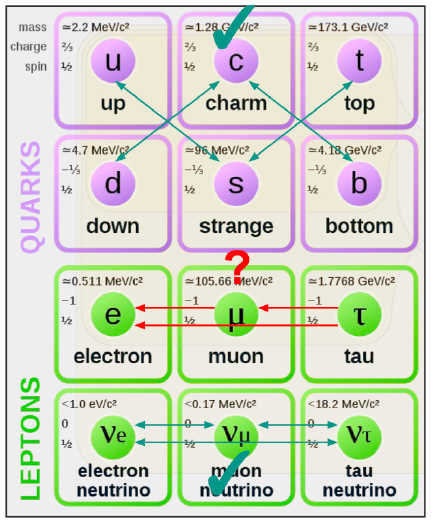
\includegraphics[width=0.7\columnwidth]{figures/png/Screenshot_20240913_102556.png}
        \end{figure} 
        
        \begin{figure}[h]
            \centering
            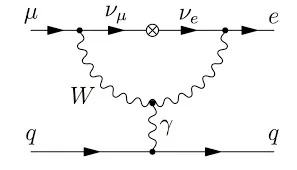
\includegraphics[width=0.7\columnwidth]{figures/jpg/1_erkKoywyuFzJmMv4PKpc9Q.jpg}
        \end{figure} 
    \end{column}
\end{columns}
\end{frame}

		%%%%%%%%%%%%%%%%%%%%%%%%%%%%%%%%%%%%%%%%
		%%  Slide 3: <ArgomentoSecondaSlide>  %%
		%%%%%%%%%%%%%%%%%%%%%%%%%%%%%%%%%%%%%%%%

%\section{Capitolo 2}
\begin{frame}
    \frametitle{Search for CLFV}
                \vspace{-2mm}

   \begin{columns}
    \begin{column}{0.63\framewidth}
        \setlength{\leftmargini}{1.3em}
        \begin{itemize}
            {\footnotesize    \item New Physics (NP) models predict much \textbf{higher rates} of CLFV $\rightarrow$ unambiguous evidence of \textbf{physics beyond the SM};
            \vspace{4mm}
            \item CLFV channels involving muons: $\mu^+ \rightarrow e^+ \gamma$, $ \mu^- N \rightarrow e^- N $ and $\mu^+ \rightarrow e^+ e^+ e^-$;
            \vspace{4mm}
            \item $ \mu^- N \rightarrow e^- N $ channel:
            }
            \vspace{1.5mm}
            \begin{itemize}
                {\footnotesize    \item Higher momentum signal;
                \vspace{1.5mm}
                \item Benefits from high intensity beam;
                \vspace{1.5mm}
                \item Better sensitivity to CLFV in a large \\ range of NP scenarios.}
            \end{itemize}
            \vspace{4mm}
            {\footnotesize    \item Current best limit on $\mu^- N \rightarrow e^- N$ by SINDRUM II: $R_{\mu e} < 7 \times 10^{-13}$ (90\% CL).}
        \end{itemize}
    \end{column}
    \begin{column}{0.5\framewidth}
        \begin{figure}[h]
            \centering
            \hspace*{-3.1ex}
            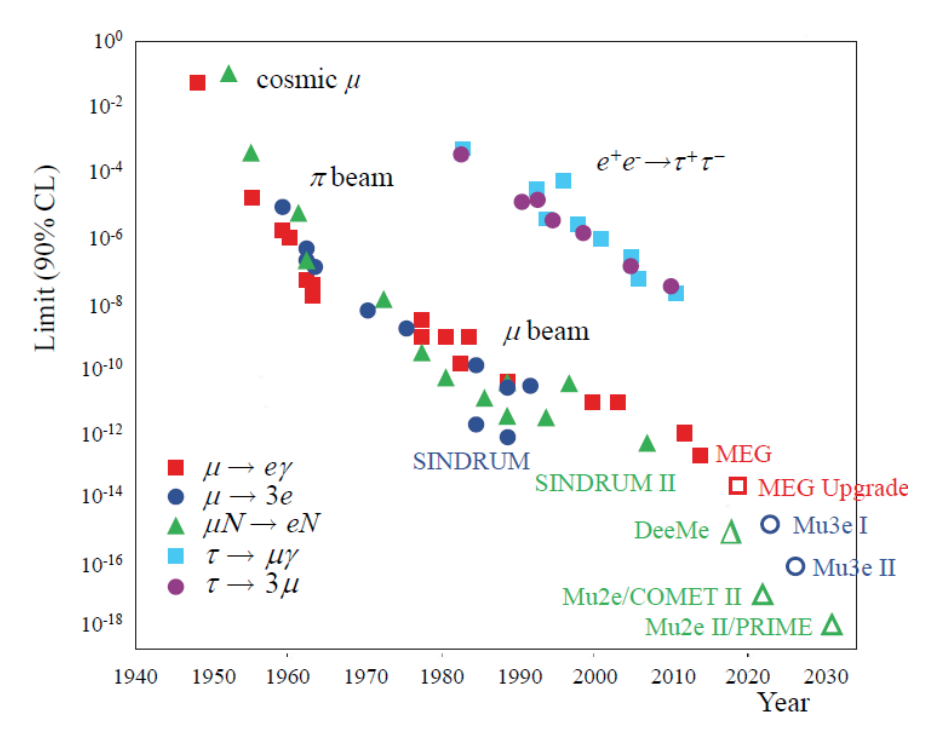
\includegraphics[width=1.1\columnwidth]{figures/png/Screenshot_20240912_093047.png}
        \end{figure}  
    \end{column}
\end{columns}
\end{frame}



        %%%%%%%%%%%%%%%%%%%%%%%%%%%%%%%%%%%%
        %% Slide 4: <ArgomentoTerzaSlide> %%
        %%%%%%%%%%%%%%%%%%%%%%%%%%%%%%%%%%%%

%\section{Capitolo 3}
\begin{frame}
    \frametitle{The Mu2e experiment}
    \vspace{-3mm}
\begin{columns}
    \begin{column}{0.63\framewidth}
        \setlength{\leftmargini}{1.3em}
        \begin{itemize}
          {\footnotesize  \item Search for neutrinoless, coherent conversion $\mu^- N \rightarrow e^- N$ in the field of an Al nucleus, by measuring: 
           \vspace{2mm}
            $$R_{\mu e}=\frac{\mu^{-}+N(Z, A) \rightarrow e^{-}+N(Z, A)}{\mu^{-}+N(Z, A) \rightarrow \nu_\mu+N(Z-1, A)}$$
            \vspace{2mm}
            \item Mu2e goal is to improve SINDRUM II limit by 4 orders of magnitude;
            \vspace{4mm}
            \item The signal is a monochromatic conversion electron (CE) with energy: 
            $$ E_{CE} = m_\mu - E_{recoil} - E_{bind} = 104.97 \ \text{MeV}$$
            where $m_\mu$ is the muon mass, $E_{recoil}$ the target nucleus recoil energy and $E_{bind}$ the muonic atom $1s$ state binding energy.}
        \end{itemize}
    \end{column}
    \begin{column}{0.5\framewidth}
    
                \begin{figure}[h]
            \centering
            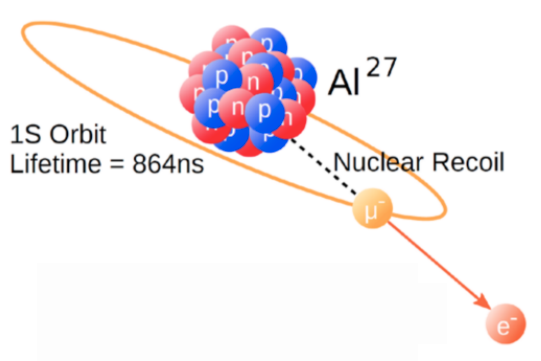
\includegraphics[width=0.75\columnwidth]{figures/png/Screenshot_20240913_160115.png}
        \end{figure} 
    \end{column}
\end{columns}
\end{frame}


\begin{frame}
    \frametitle{Background sources}
            \vspace{-3mm} 

         \begin{figure}[h]
            \centering
            \hspace*{-4ex}
            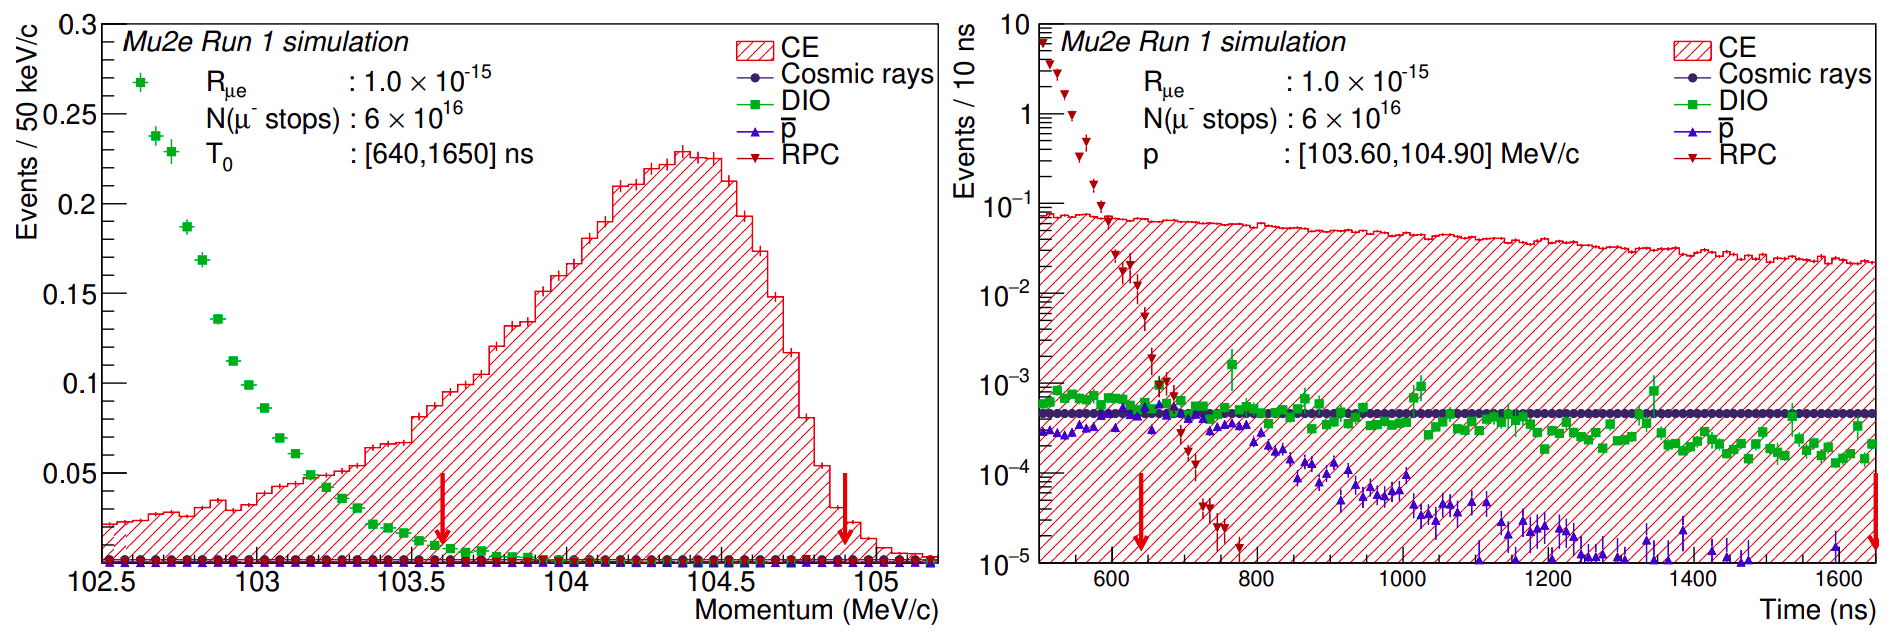
\includegraphics[width=1.\framewidth]{figures/png/Screenshot_20240225_102708.png}
        \end{figure}
        \setlength{\leftmargini}{-0.5em}
        \vspace{-3mm} 
      
    \begin{itemize}
      {\footnotesize
    \item \textbf{Cosmics} $\rightarrow$ veto enclosing the detector {\footnotesize($\approx$0.046 evs/RunI)};   
\item \textbf{Intrinsic} $\rightarrow$ 1 MeV/c momentum resolution:}
\begin{itemize}
    {\footnotesize\item Decay In Orbit $\mu^- N \rightarrow e^- \bar{\nu}_e\nu_\mu N $ {\footnotesize($\approx$0.038 evs/RunI)};
 \item Radiative Muon Capture $\mu^- N \rightarrow\gamma \nu_\mu N'* $ {\footnotesize($<0.0024$ evs/RunI)}.}
\end{itemize}
{\footnotesize \item \textbf{Delayed processes from $\bar{p}$} $\rightarrow$ absorbers in the TS {\footnotesize($\approx0.010$ evs/RunI)};
\item \textbf{Prompt processes} $\rightarrow$ pulsed beam (1.7 $\mu$s) + 640 ns delayed window:}
\begin{itemize}
    {\footnotesize  \item Radiative Pion Capture $\pi^- N \rightarrow \gamma N' *$ {\footnotesize($\approx0.010$ evs/RunI)};
 \item $\pi$ and $\mu$ Decay In Flight {\footnotesize($<2\times 10^{-3}$ evs/RunI)};
 \item Beam electrons {\footnotesize($<1\times 10^{-3}$ evs/RunI)}.}
     \end{itemize}
       
      \end{itemize}
\end{frame}

\begin{frame}
    \frametitle{The Mu2e experimental setup}
    \vspace{-7mm}
     \begin{figure}[h!]
            \centering
            \hspace*{-4ex}
            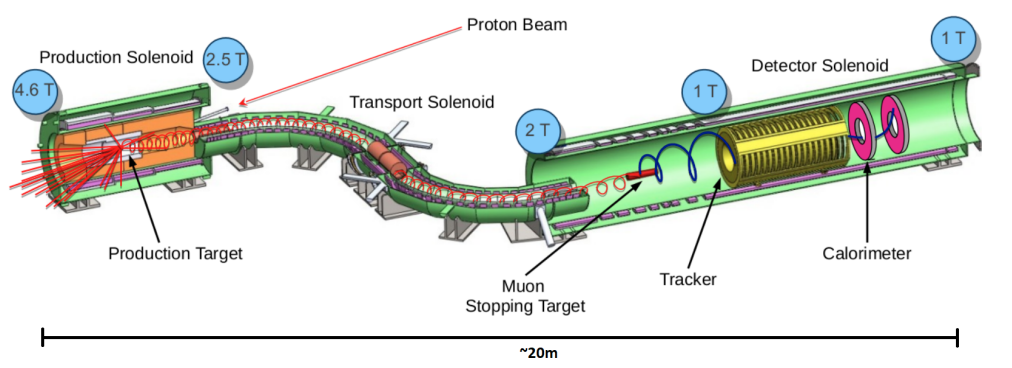
\includegraphics[width=1.1\framewidth, height=3.5cm]{figures/png/Screenshot_20240913_162936.png}
        \end{figure}
                \setlength{\leftmargini}{-0.5em}
\vspace{-2mm}
        \begin{itemize}
        {\footnotesize
            \item \textbf{Production Solenoid}:}
            \begin{itemize}
                {\footnotesize  \item 8 GeV pulsed proton beam interacts with the W target and mostly $\pi$s are produced;
                \item graded field for backward collection.}
            \end{itemize}
            {\footnotesize \item \textbf{Transport Solenoid}:}
            \begin{itemize}
                {\footnotesize \item it allows for $\pi$ decay and $\mu$ transport;
                \item $S$-shape for charged particle selection;
                \item it selects muons with $p \lesssim 100 $ MeV/c;
                \item rotating collimator COL3 selects $\mu^-$ or $\mu^+$ beam.}
            \end{itemize}
\item  {\footnotesize \textbf{Detector Solenoid}: } 
\begin{itemize}
    {\footnotesize  \item Al Stopping Target, $p$ absorber, tracker and calorimeter.}
\end{itemize}
        \end{itemize}
\end{frame}

\begin{frame}
    \frametitle{The straw tracker}
    \begin{columns}
    \begin{column}{0.65 \framewidth}
{\footnotesize \textbf{Purpose}:}
\vspace{0.5mm}
\begin{itemize}
    {\footnotesize \item momentum measurement with $\sigma_p<300$ keV/c FWHM + 950 keV/c energy losses (ST and proton absorber). }
    \vspace{2mm}
\end{itemize}
{\footnotesize \textbf{Design}:}
\vspace{1mm}
\begin{itemize}
    {\footnotesize
    \item 5 mm diameter and 40-110 cm long straws filled with a 80\%:20\% Ar:CO$_2$ mixture at a pressure of 1 atm;
    \vspace{2mm}
    \item 3 m downstream of the ST (B$\sim$1 T);
    \vspace{2mm}
    \item hollow geometry (low $p_T$ particles);
    \vspace{2mm}
    \item 96 straws per panel, 3 panels per face, 2 faces per plane, 2 planes per station;
    \vspace{2mm}
        \item 18 tracking stations: 216 panels;
        \vspace{2mm}
        \item 3 m long tracker in vacuum.}
       
        
        
    \end{itemize}
    
    \end{column}
    \begin{column}{0.5 \framewidth}
    \vspace{-10mm}
      \begin{figure}[h!]
          \centering
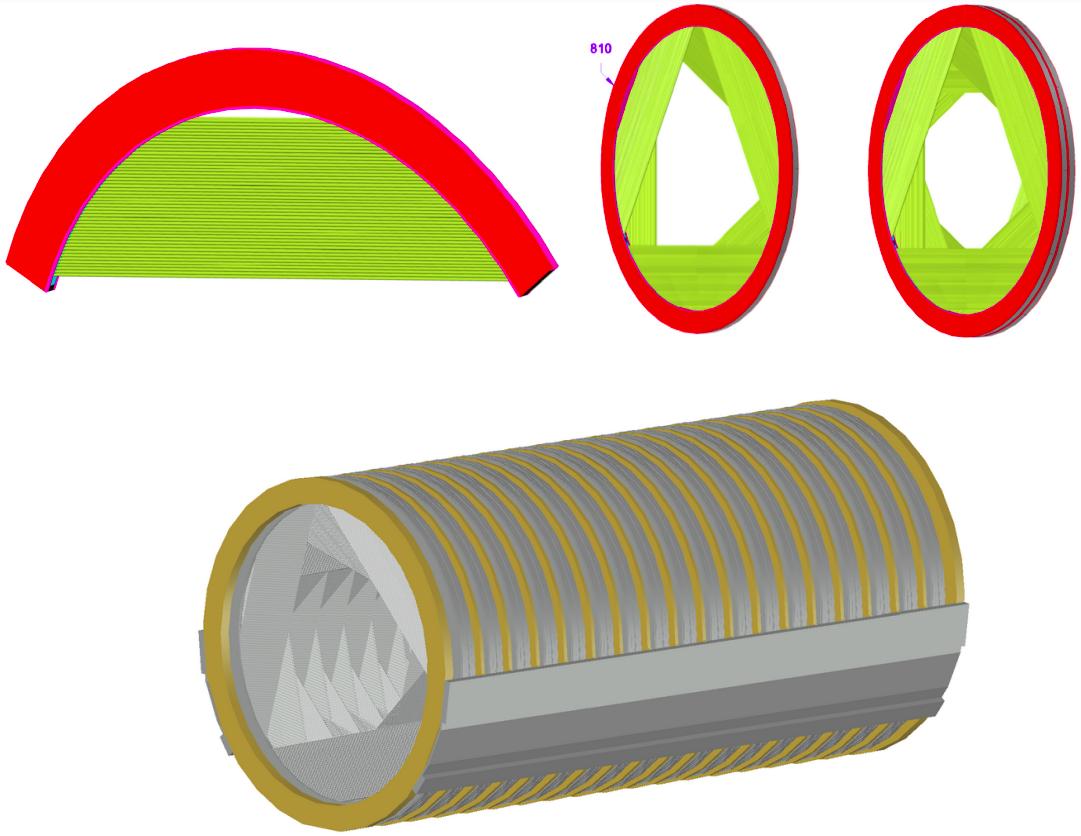
\includegraphics[width=0.8\columnwidth]{figures/png/Screenshot_20240306_222803.png}
          \label{fig:enter-label} 
      \end{figure}
     \begin{figure}[h!]
          \centering
            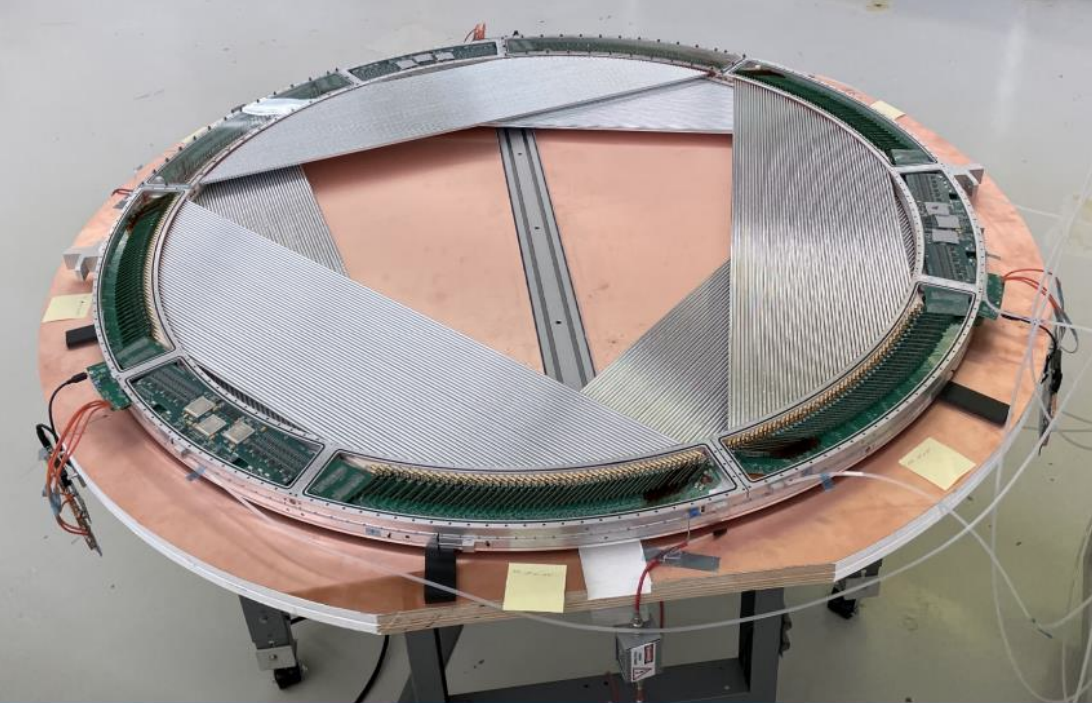
\includegraphics[width=0.8\columnwidth]{figures/png/Screenshot_20240706_163056.png}
          \label{fig:enter-label} 
      \end{figure}
    \end{column}
    \end{columns}
    \end{frame}
\begin{frame}
    \frametitle{The tracker readout and DAQ}
    \vspace{-6mm}
    \begin{columns}
         \begin{column}{0.6\framewidth}
         \setlength{\leftmargini}{1em}
         \begin{itemize}
         {\footnotesize
         \item Signal is readout from both ends by  \textbf{preamps};
         \vspace{5mm}
         \item Analog signals are sent to the \\ \textbf{DRAC} (Digitizer Readout and \\
         Assembler Controller) and processed \\ by 2 \textbf{TDC}s and one \textbf{ADC};
         \vspace{5mm}
        \item The 2 digi-FPGA create one data \\ packet for each hit with \textbf{two hit} \\ \textbf{times} and \textbf{one waveform};
        \vspace{5mm}
        \item Data packets sent to \textbf{ROC} (Readout Controller);
        \vspace{5mm}
        \item ROC transfers data from digi-FPGAs \\ to \textbf{DTC} (Data Transfer Controller) \\ installed on \textbf{DAQ} computers.}
         \end{itemize}
    \end{column}
    \begin{column}{0.5\framewidth}
           \begin{figure}[h]
          \centering
                    \hspace*{-1.2em}
            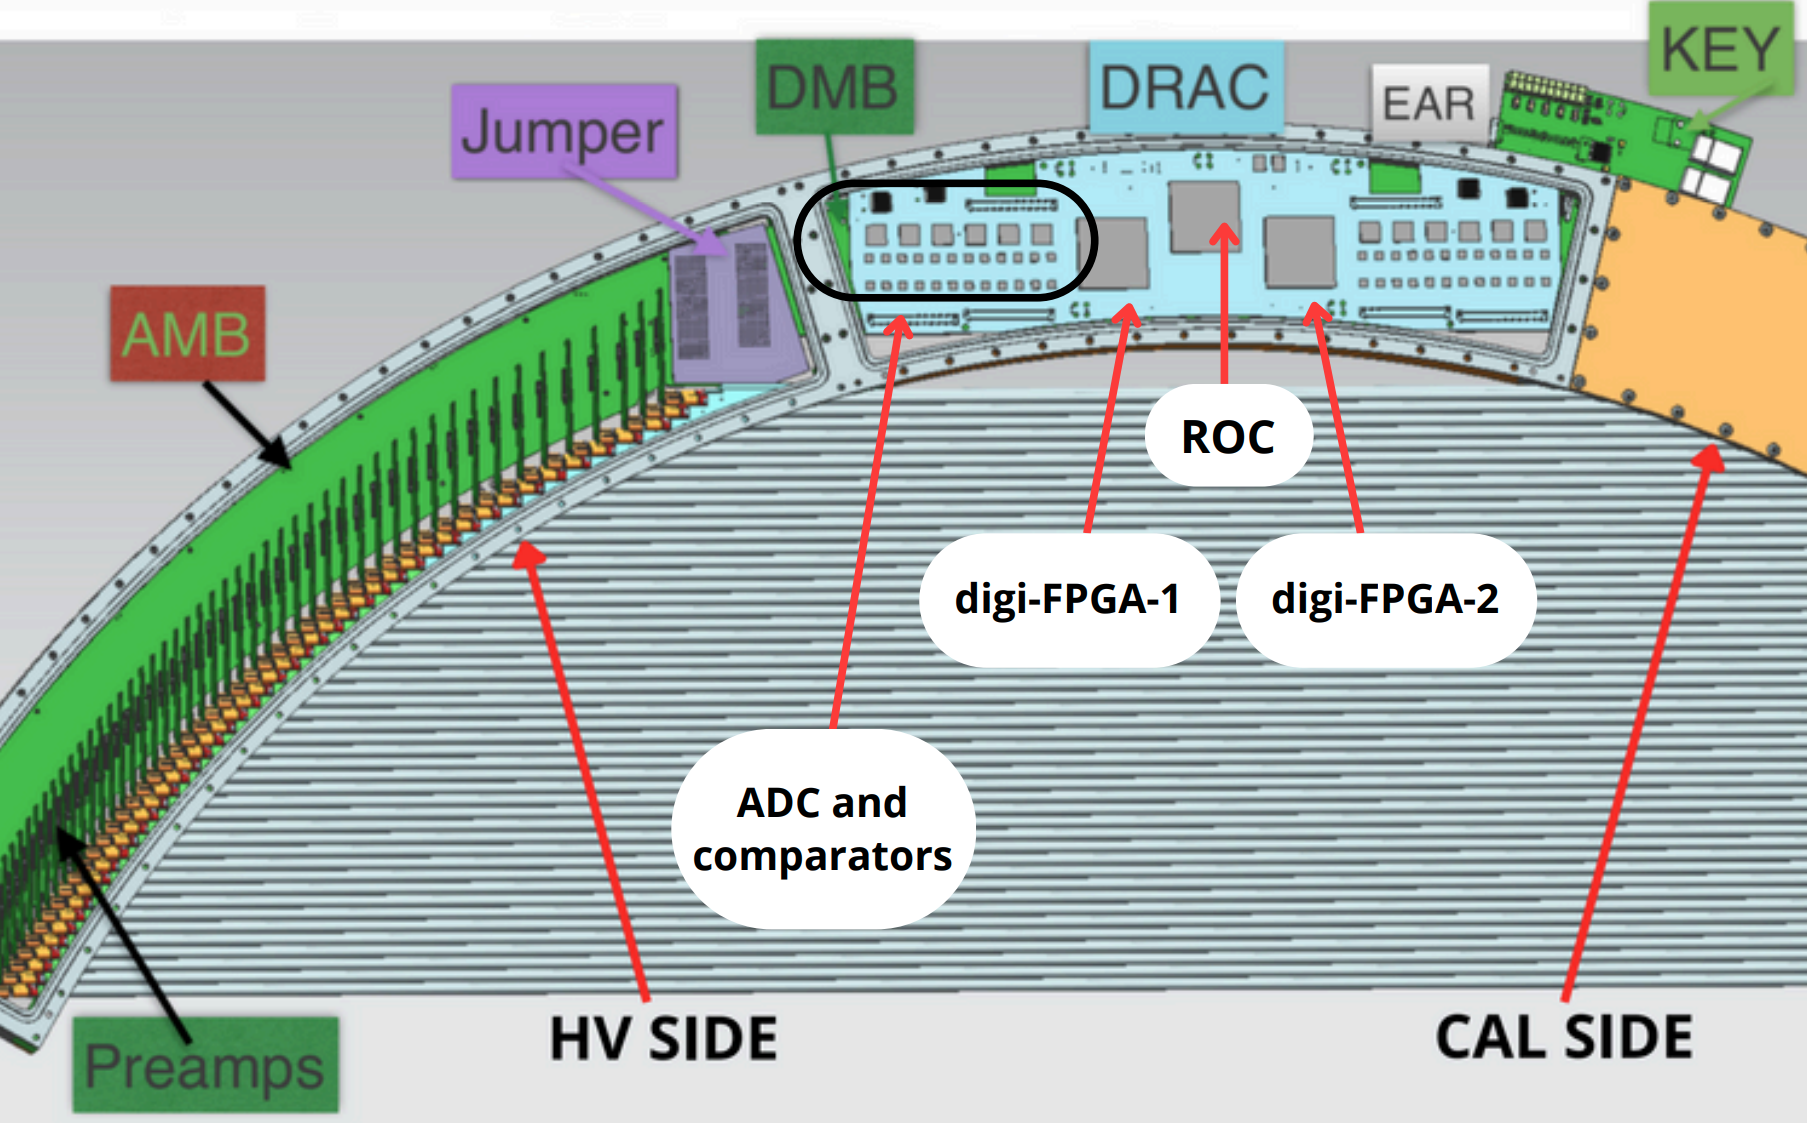
\includegraphics[width=1.1\columnwidth]{figures/png/Screenshot_20240919_110354.png}
          \label{fig:enter-label} 
      \end{figure} 
           \begin{figure}[h]
          \centering
          \vspace{-10mm}
            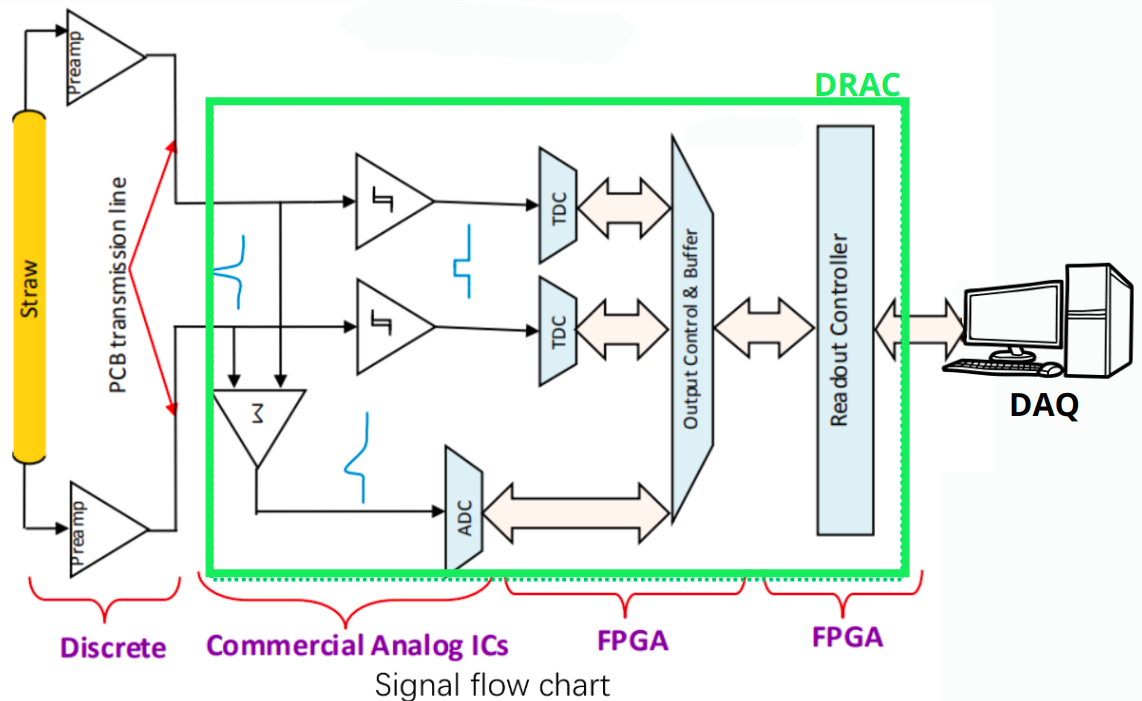
\includegraphics[width=1.02\columnwidth]{figures/png/Screenshot_20240529_133230.png}
          \label{fig:enter-label} 
      \end{figure} 
    \end{column}
    \end{columns}

\end{frame}
\begin{frame}
    \frametitle{My Thesis}
    
\begin{columns}
   \begin{column}{1.15\framewidth} 
         \setlength{\leftmargini}{1.3em}
\vspace{-4mm}
\begin{itemize}
    {\footnotesize \item Mu2e is starting detector \textbf{commissioning} and \textbf{calibration};}
     \vspace{9mm}
     {\footnotesize \item My work consists of a \textbf{comprehensive study of the Mu2e tracker}:}
\vspace{9mm}
  \begin{itemize}
    {\footnotesize \item \textbf{Vertical Slice Test} (VST). The entire 
testing chain, from the straws to the readout, to processed data on disk;}

     \vspace{9mm}

     {\footnotesize \item First steps towards the tracker timing \textbf{calibration} with \textbf{cosmics};}
   
         \vspace{9mm}

         {\footnotesize \item \textbf{Mu2e Offline}. Pre-pattern recognition studies.}
        
        \end{itemize}
\end{itemize}
 \end{column}
 \end{columns}
     

\end{frame}
\begin{frame}
    \frametitle{Outline}
    
\begin{itemize}
\item Commissioning of the tracker DAQ and FEE:
\begin{itemize}
         \vspace{2mm}

    \item validation of ROC readout;
             \vspace{1.5mm}

    \item \textcolor{mygray}{study of preamplifiers performance}.
\end{itemize}
\vspace{4mm}
    \item \textcolor{mygray}{First steps towards the station calibration;}
    \vspace{6mm}

    \item \textcolor{mygray}{Pre-pattern recognition studies;}
   \vspace{6mm}

    \item \textcolor{mygray}{Conclusions.}
\end{itemize}
\end{frame}

 \begin{frame}{Test stand and data taking logic}
 \vspace{-3.5mm}
\begin{columns}
    \begin{column}{0.69\framewidth}
             \setlength{\leftmargini}{1.3em}
      \begin{itemize}
    {\footnotesize 
          \item \textbf{Tracker test stand}: 1 ROC (1 panel-96 channels), 1 DTC installed on DAQ computer;
            
          \vspace{3mm}
          \item Each FPGA has its own generator ($f_{gen}$) and they are offset ($\in [0 ,T_{gen}]$) wrt each other;
          \vspace{3mm}
          \item Channel offsets (same digi-FPGA) are few ns;
          \vspace{3mm}
          \item \textbf{Event Window} ($T_{EW}$): time between two proton pulses (1.7 $\mu$s), varied $\in$(0.7, 50) $\mu$s;
          \vspace{3mm}
            \item Depending on $T_{gen}=1/f_{gen}$ and $T_{EW}$, data taking can proceed in 2 modes:}
    \vspace{1mm}
\begin{itemize}

    {\footnotesize\item $N_{gen}\geq255$: $N_{read}=255$ (\textbf{overflow});
    \vspace{1mm}
  \item $N_{gen}<255$: $N_{read}<255$ (\textbf{regular}).}
\end{itemize}
{\footnotesize
\vspace{3mm}
\item Pulse generator uncorrelated with the EW;
\vspace{3mm}
\item Channel readout sequence is fixed.

}
      \end{itemize}
          \end{column}
\begin{column}{0.45\framewidth}
        \begin{figure}[h]
          \centering
            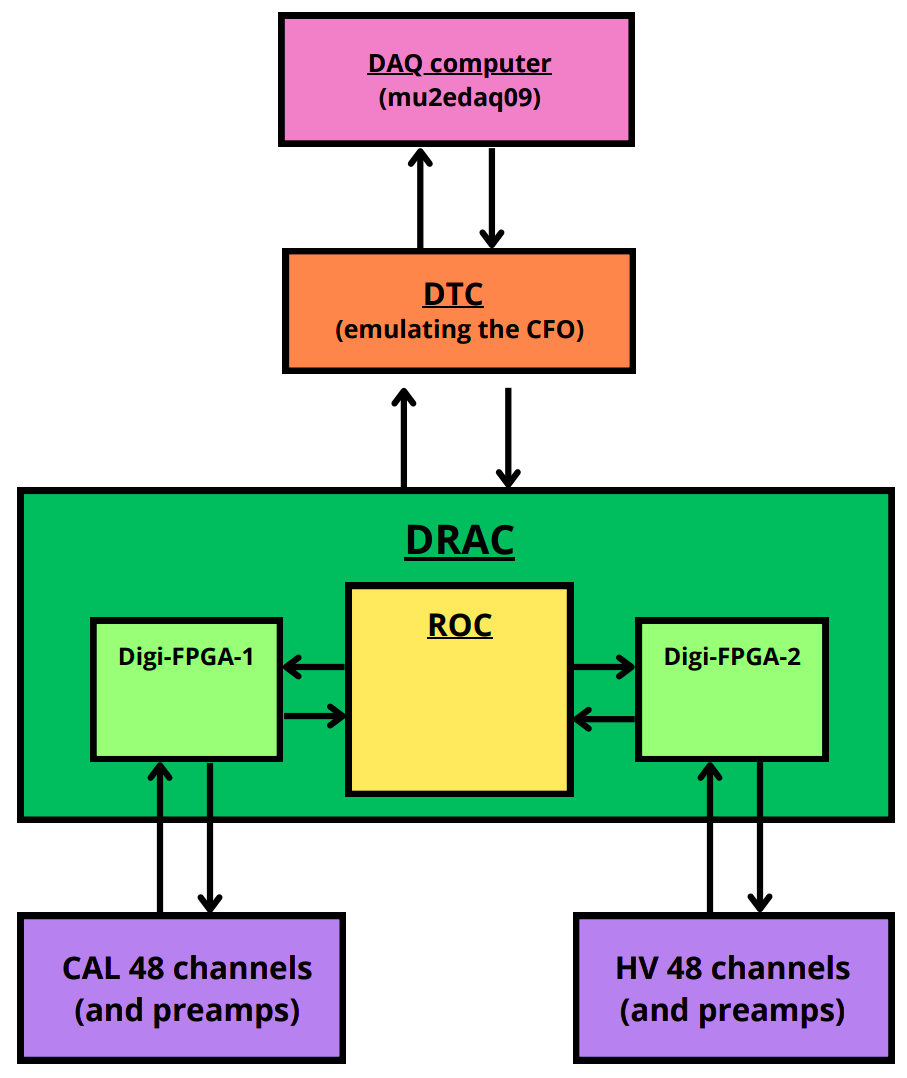
\includegraphics[width=0.7\columnwidth]{figures/png/Screenshot_20240712_102528.png}
          \label{fig:enter-label} 
      \end{figure} 
      \vspace{-4mm}
      \begin{figure}[h!]
        \centering
        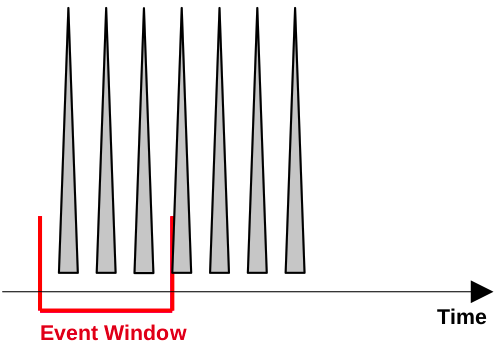
\includegraphics[width=0.55\columnwidth]{figures/png/Screenshot_20241013_113750.png}
        \label{fig:enter-label} 
    \end{figure}
    \vspace{-5mm}
      \begin{figure}[h!]
        \centering
        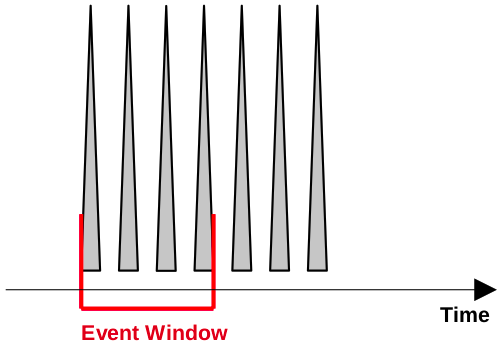
\includegraphics[width=0.55\columnwidth]{figures/png/Screenshot_20241013_113809.png}
        \label{fig:enter-label} 
    \end{figure}
\end{column}
\end{columns}




          \end{frame}




\begin{frame}{Monte Carlo simulation}


   \vspace{-3mm}
   \begin{columns}
 \begin{column}{0.65\framewidth} 

       \begin{itemize}
       {\footnotesize
           \item ROC readout logic emulated with a bit-level C++ simulation;
           \vspace{0.8mm}
           \item Simulated parameters:
          \vspace{0.8mm}
           \begin{itemize}
            {\footnotesize  \item $N_{hits}$ in each channel;
               \item $N_{read}$ per event.}
           \end{itemize}
          \vspace{0.8mm}
           \item digi-FPGAs and channel-to-channel offsets. }
       \end{itemize}
      \vspace{0.8mm}
      {\footnotesize  \textbf{Steps of the simulation:}}
     \vspace{0.8mm}
\begin{itemize}
{\footnotesize
\item EW starts at $t=0$ s;
\vspace{0.8mm}
 \item The 1st pulse is generated $T_0\in [0 ,T_{gen}]$;
\vspace{0.8mm}
   \item Next pulses: $T_i = T_{i-1} + T_{gen}$, until $T_i> T_{EW}$;
   \vspace{0.8mm}
\item Pulses are generated in each channel following the readout sequence;
\vspace{0.8mm}
 \item The procedure \textit{continues} until all hits 
 have been $readout$, or $N_{read}>255$. }
\end{itemize}
   \end{column}
   \begin{column}{0.5\framewidth}
    \begin{figure}[h!]
        \centering
    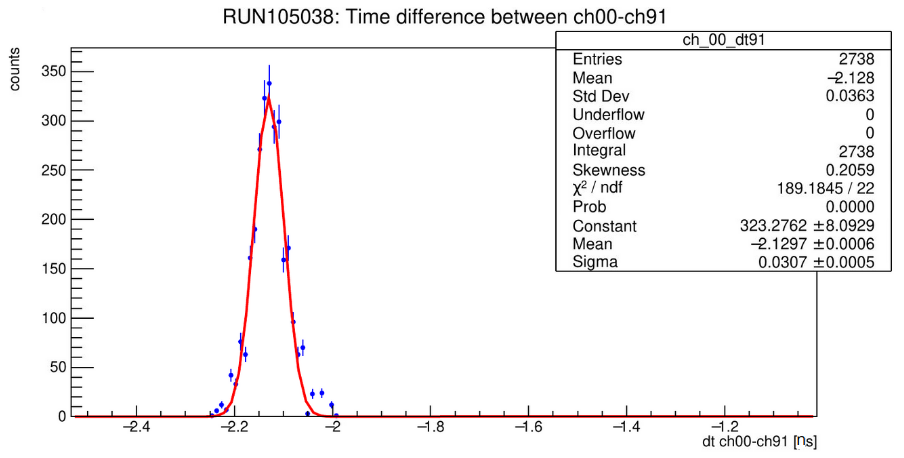
\includegraphics[width=\columnwidth]{figures/png/Screenshot from 2023-12-03 11-50-50.png}
    \label{fig:delay1}
  \end{figure}
  \begin{figure}[h!]
        \centering
    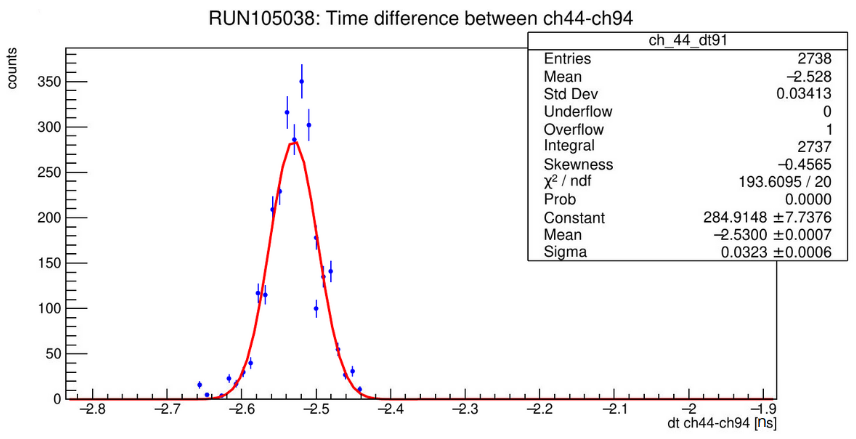
\includegraphics[width=\columnwidth]{figures/png/Screenshot from 2023-12-03 11-50-33.png}

    \label{fig:delay2}
  \end{figure}
   \end{column}
  \end{columns}



    \end{frame}

    


    \begin{frame}{Hit timing distribution}
        \vspace{-3mm}
        \begin{columns}
            \begin{column}{0.5\framewidth}
                \begin{figure}[h!]
                  \centering
                  \hspace*{-2em}
                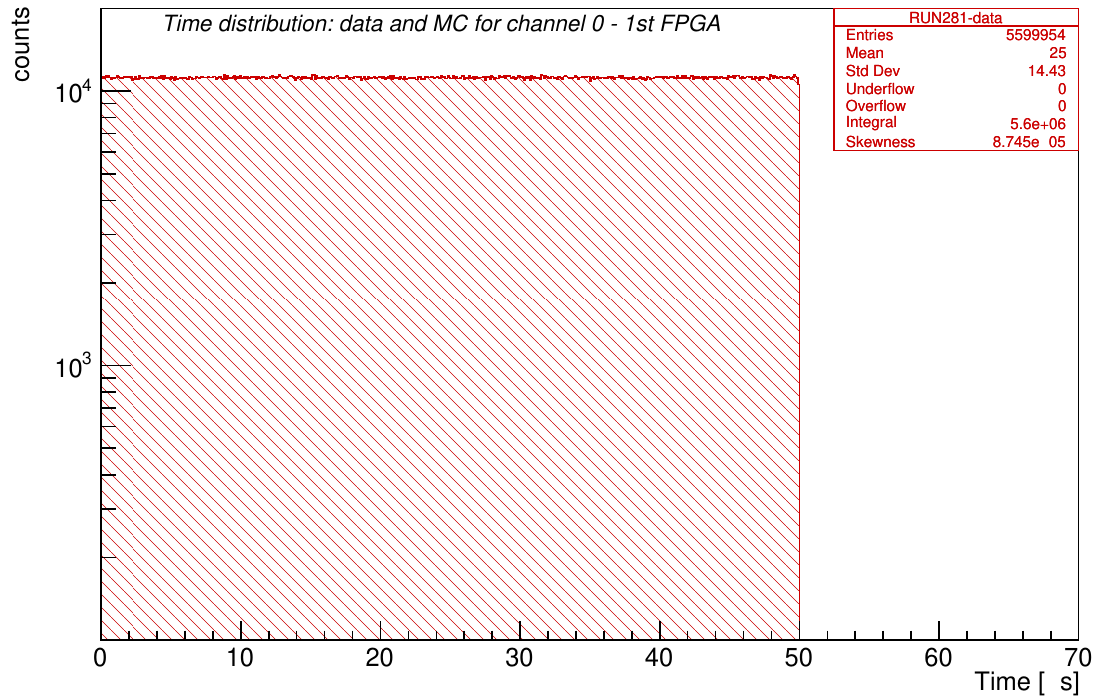
\includegraphics[width=0.85\columnwidth]{figures/png/Screenshot_20241013_115510.png}
                  \label{fig:enter-label} 
                  \end{figure}
                  \vspace{-4mm}
                  \begin{figure}[h!]
                    \centering
                    \hspace*{-2em}
                  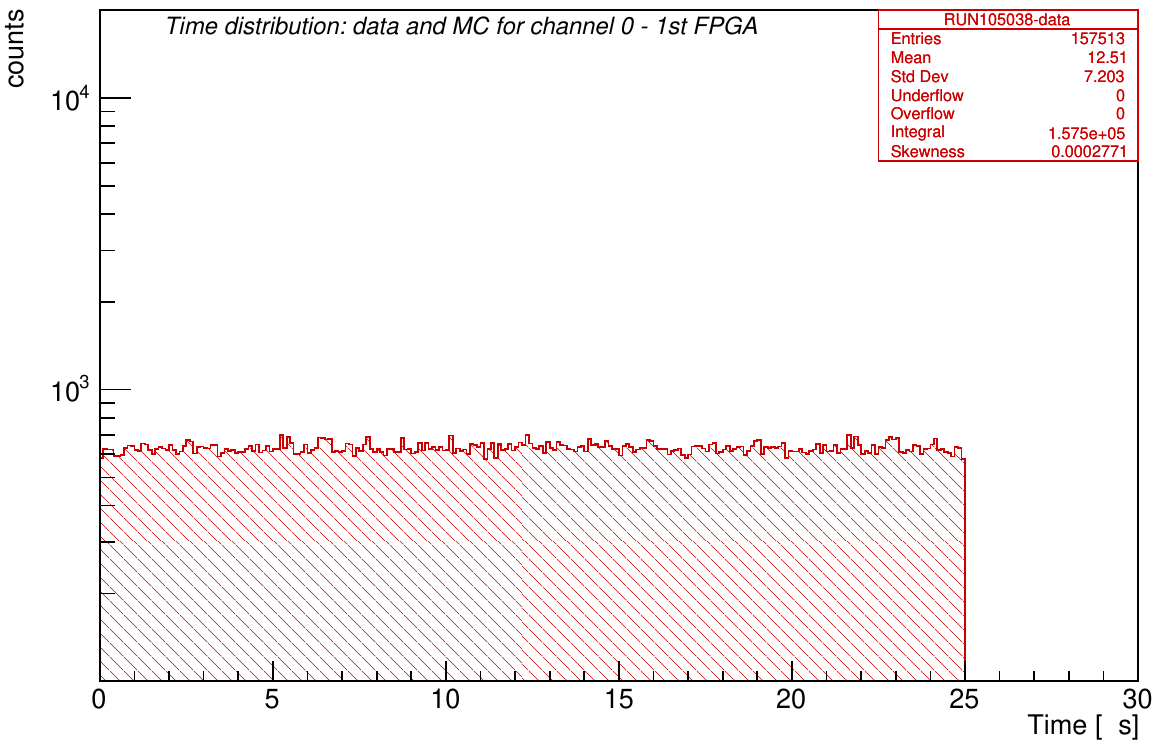
\includegraphics[width=0.85\columnwidth]{figures/png/Screenshot_20241013_115638.png}
                    \label{fig:enter-label} 
                    \end{figure}
            \end{column}
            \begin{column}{0.5\framewidth}
                \begin{figure}[h!]
                  \centering
                            \hspace*{-1em}
                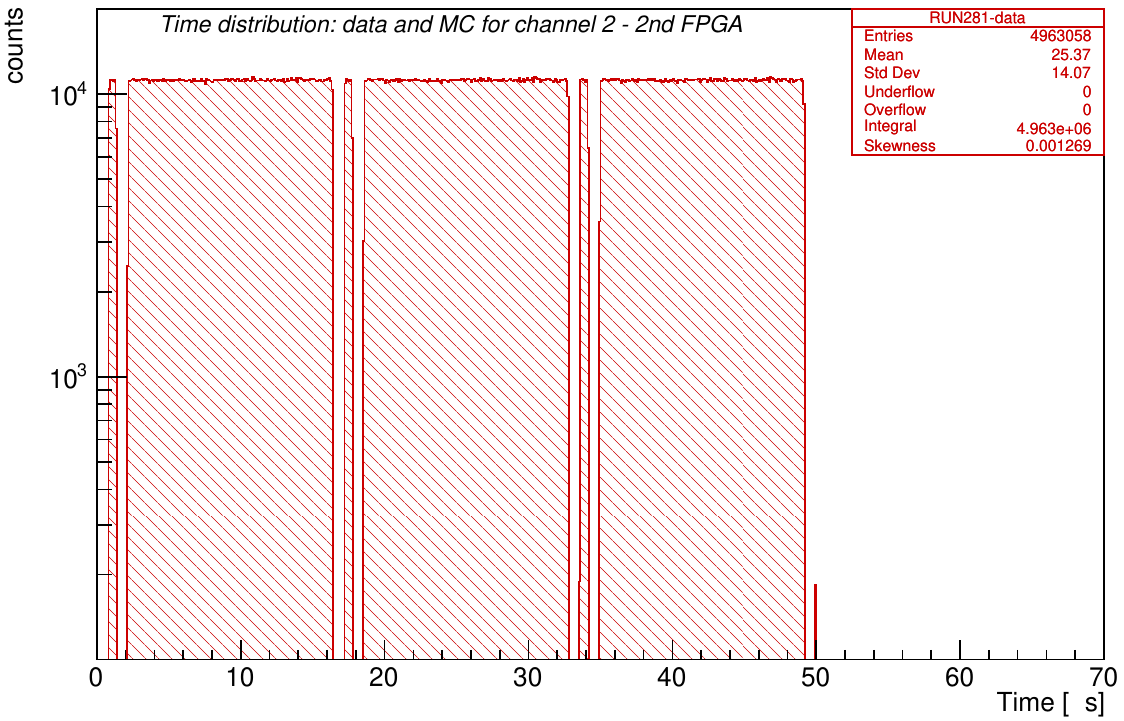
\includegraphics[width=0.85\columnwidth]{figures/png/Screenshot_20241013_115554.png}
                  \label{fig:enter-label} 
                  \end{figure} 
                  \vspace{-4mm}
                  \begin{figure}[h!]
                    \centering
                              \hspace*{-1em}
                  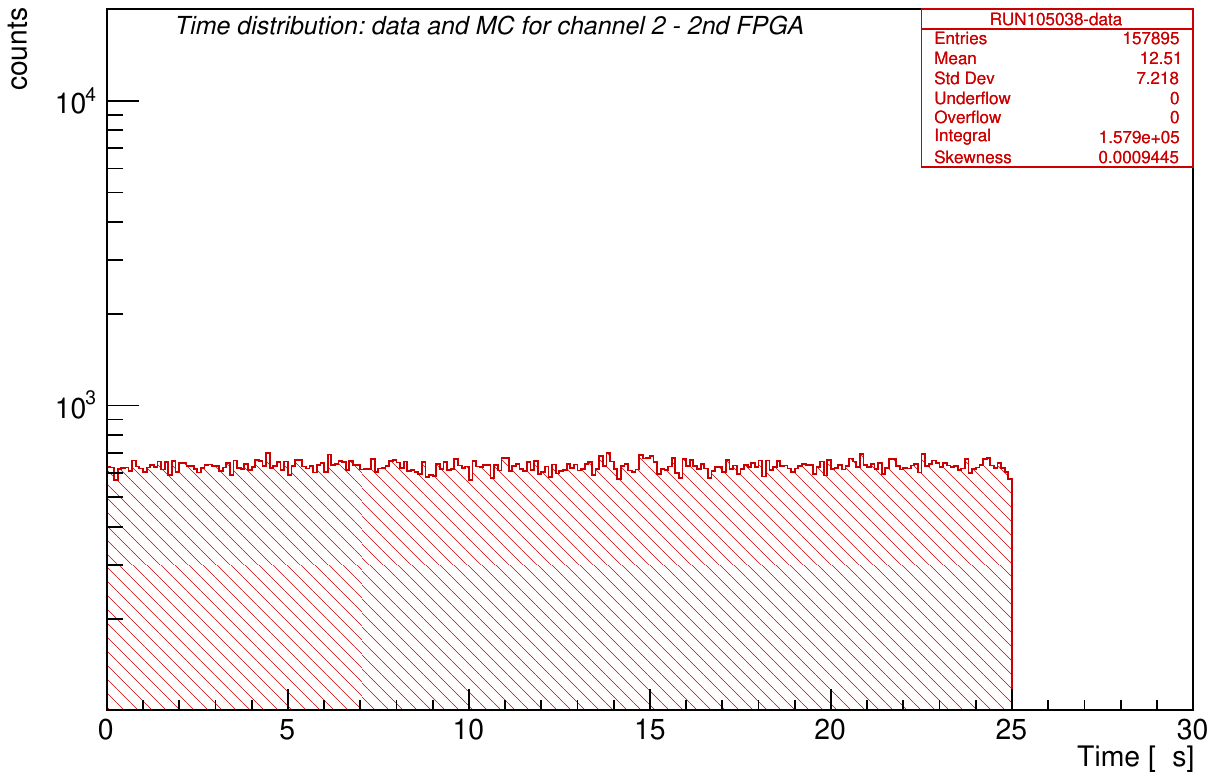
\includegraphics[width=0.85\columnwidth]{figures/png/Screenshot_20241013_115705.png}
                    \label{fig:enter-label} 
                    \end{figure} 
            \end{column}
        \end{columns}
        \begin{columns}

            \begin{column}{1.15\framewidth}
                \setlength{\leftmargini}{1.3em}

            \vspace{-0.5mm}
        
             \begin{itemize}
           {\footnotesize 
            \item Hit timing distribution. (Left): CH0, digi-FPGA-1. (Right): CH2, digi-FPGA-2;
             \item (Top): $T_{EW}$=50 $\mu$s and $f_{gen}$=60 kHz. (Bottom): $T_{EW}$=25 $\mu$s and $f_{gen}$=60 kHz;
             \item Different behaviour in different channels in different FPGAs;
             \vspace{-1mm}
                \item Interruptions of CH2 of digi-FPGA-2 in certain configurations.   }    
                 \end{itemize}
                 \end{column}
        \end{columns}   
    \end{frame}

    









\begin{frame}{$Occupancy$ distribution}
\vspace{-4.4mm}
\begin{columns}
    \begin{column}{0.5 \framewidth}
    \begin{figure}[h!]
          \centering
          \hspace*{-2em}
        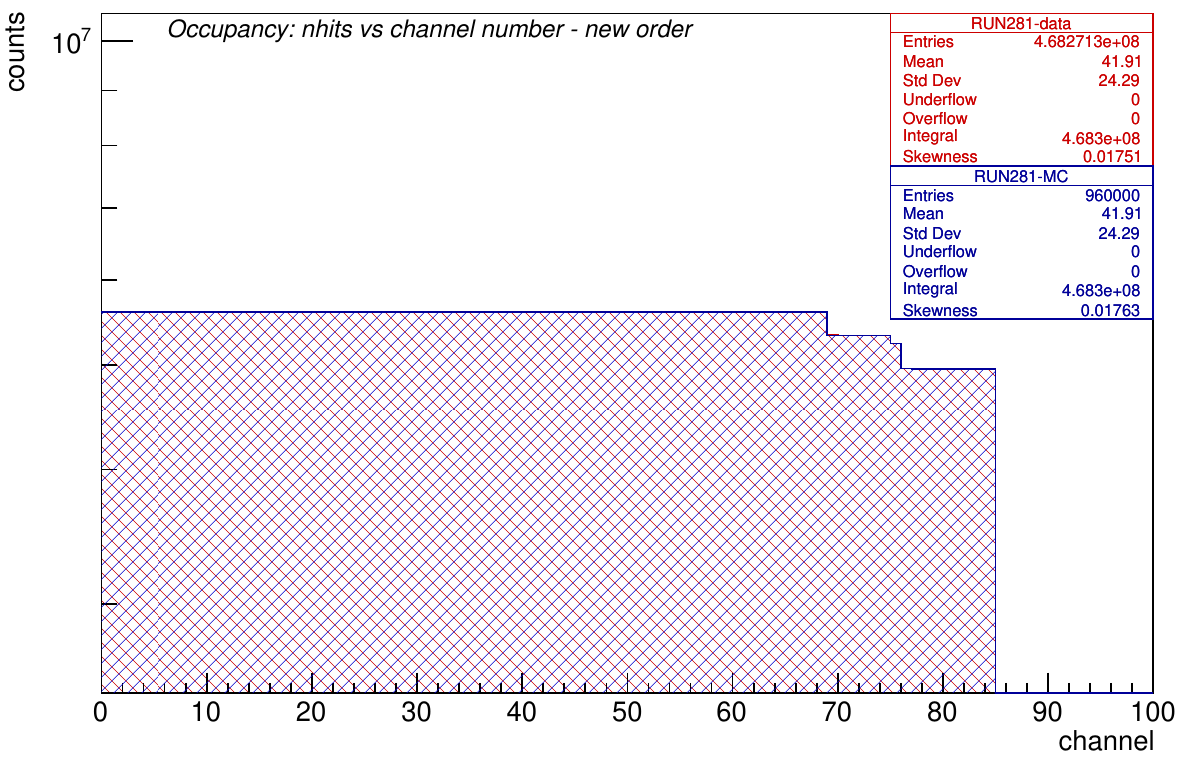
\includegraphics[width=1\columnwidth]{figures/png/Screenshot_20241013_153753.png}
          \label{fig:dfjkdsfh} 
\end{figure}    
    \end{column}
    \begin{column}{0.5 \framewidth}
           \begin{figure}[h!]
          \centering
          \hspace*{-2em}
        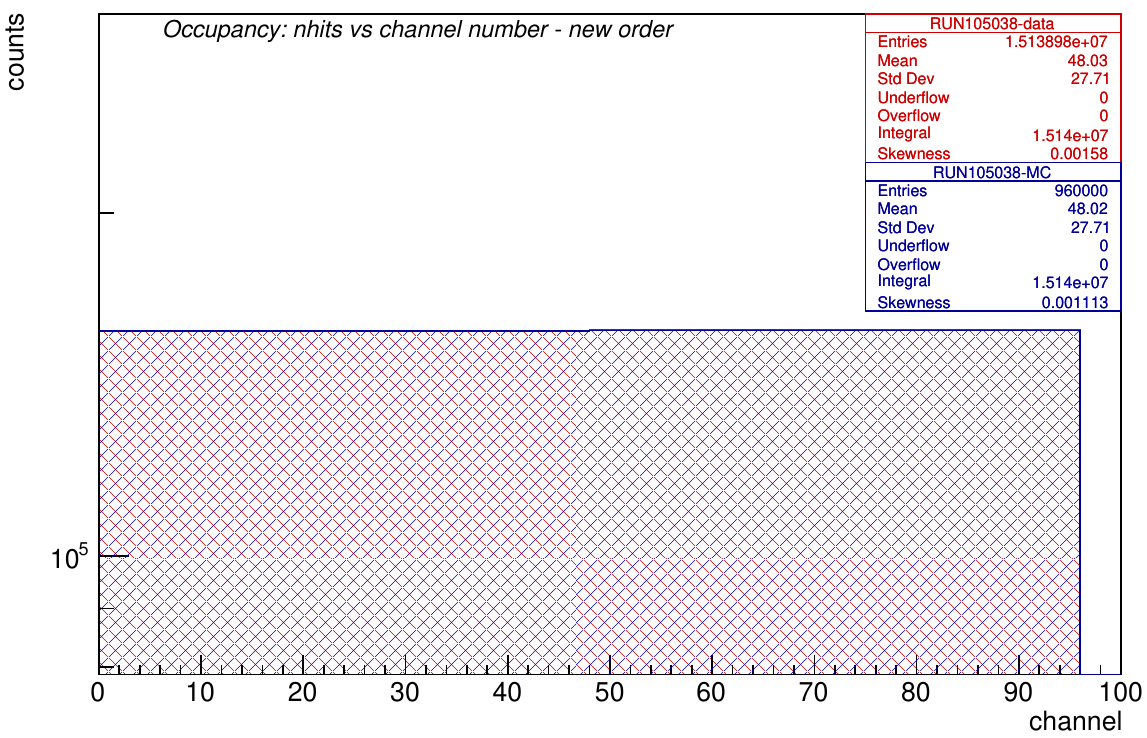
\includegraphics[width=1\columnwidth]{figures/png/Screenshot_20241013_153707.png}
          \label{fig:dfjkdsfh} 
\end{figure} 
    \end{column}
\end{columns}      
 \begin{columns}
    \begin{column}{1.17\framewidth}
        \setlength{\leftmargini}{1.2em}
     \begin{itemize}
     {\footnotesize
      \item $Occupancy$ plot: number of hits versus channel number (data red, MC blue);
    \item Overflow mode (Left):   }
    \begin{itemize}
    {\footnotesize
        \item channels 0-68: 48 digi-FPGA-1 channels with 4 hits (192 hits) and 21 digi-FPGA-2 channels with 3 hits (63 hits);
        \item channels 0-75: 48 digi-FPGA-1 channels with 3 hits (144 hits) and 27 digi-FPGA-2 channels with 4 hits (108 hits) and 1 with 3 hits (111 hits);
        \item channels 0-85: 48 digi-FPGA-1 channels with 3 hits (144 hits) and 37 digi-FPGA-2 channels with 3 hits (111 hits).}
    \end{itemize}
    {\footnotesize \item  Regular mode (Right). Number of hits per channel $\rightarrow$ EW and digi-FPGAs offset;
        \vspace{-0.5mm}
    \item Agreement between MC and data at a level of $10^{-3}$.
    }
   
        \end{itemize}
             \end{column}
\end{columns}     
\end{frame}







\begin{frame}
    \frametitle{Outline}
    
\begin{itemize}
\item Commissioning of the tracker DAQ and FEE:
\begin{itemize}
         \vspace{2mm}

    \item \textcolor{mygray}{validation of ROC readout;}
             \vspace{1.5mm}

    \item study of preamplifiers performance.
\end{itemize}
\vspace{4mm}
    \item \textcolor{mygray}{First steps towards the station calibration;}
    \vspace{6mm}

    \item \textcolor{mygray}{Pre-pattern recognition studies;}
    \vspace{6mm}

    \item \textcolor{mygray}{Conclusions.}
\end{itemize}
\end{frame}




\begin{frame}
    \frametitle{Test 1: channel occupancy}
    \vspace{-3mm}
    \begin{columns}
\begin{column}{1.15\framewidth}
    \setlength{\leftmargini}{1.2em}
 \begin{itemize}
{\footnotesize  \item Same test stand: 1 or 2 ROCs and one DTC + CAL side preamps;
\vspace{-0.7mm}
\item  Calibration pulses (every 8th channel across 12 RUNs): cross talks.}
  \end{itemize}
    \end{column}
    \end{columns}
        \vspace{-3mm}
    \begin{columns}
\begin{column}{0.5\framewidth}
         \begin{figure}[!h]
      \centering
      \hspace*{-2em}
      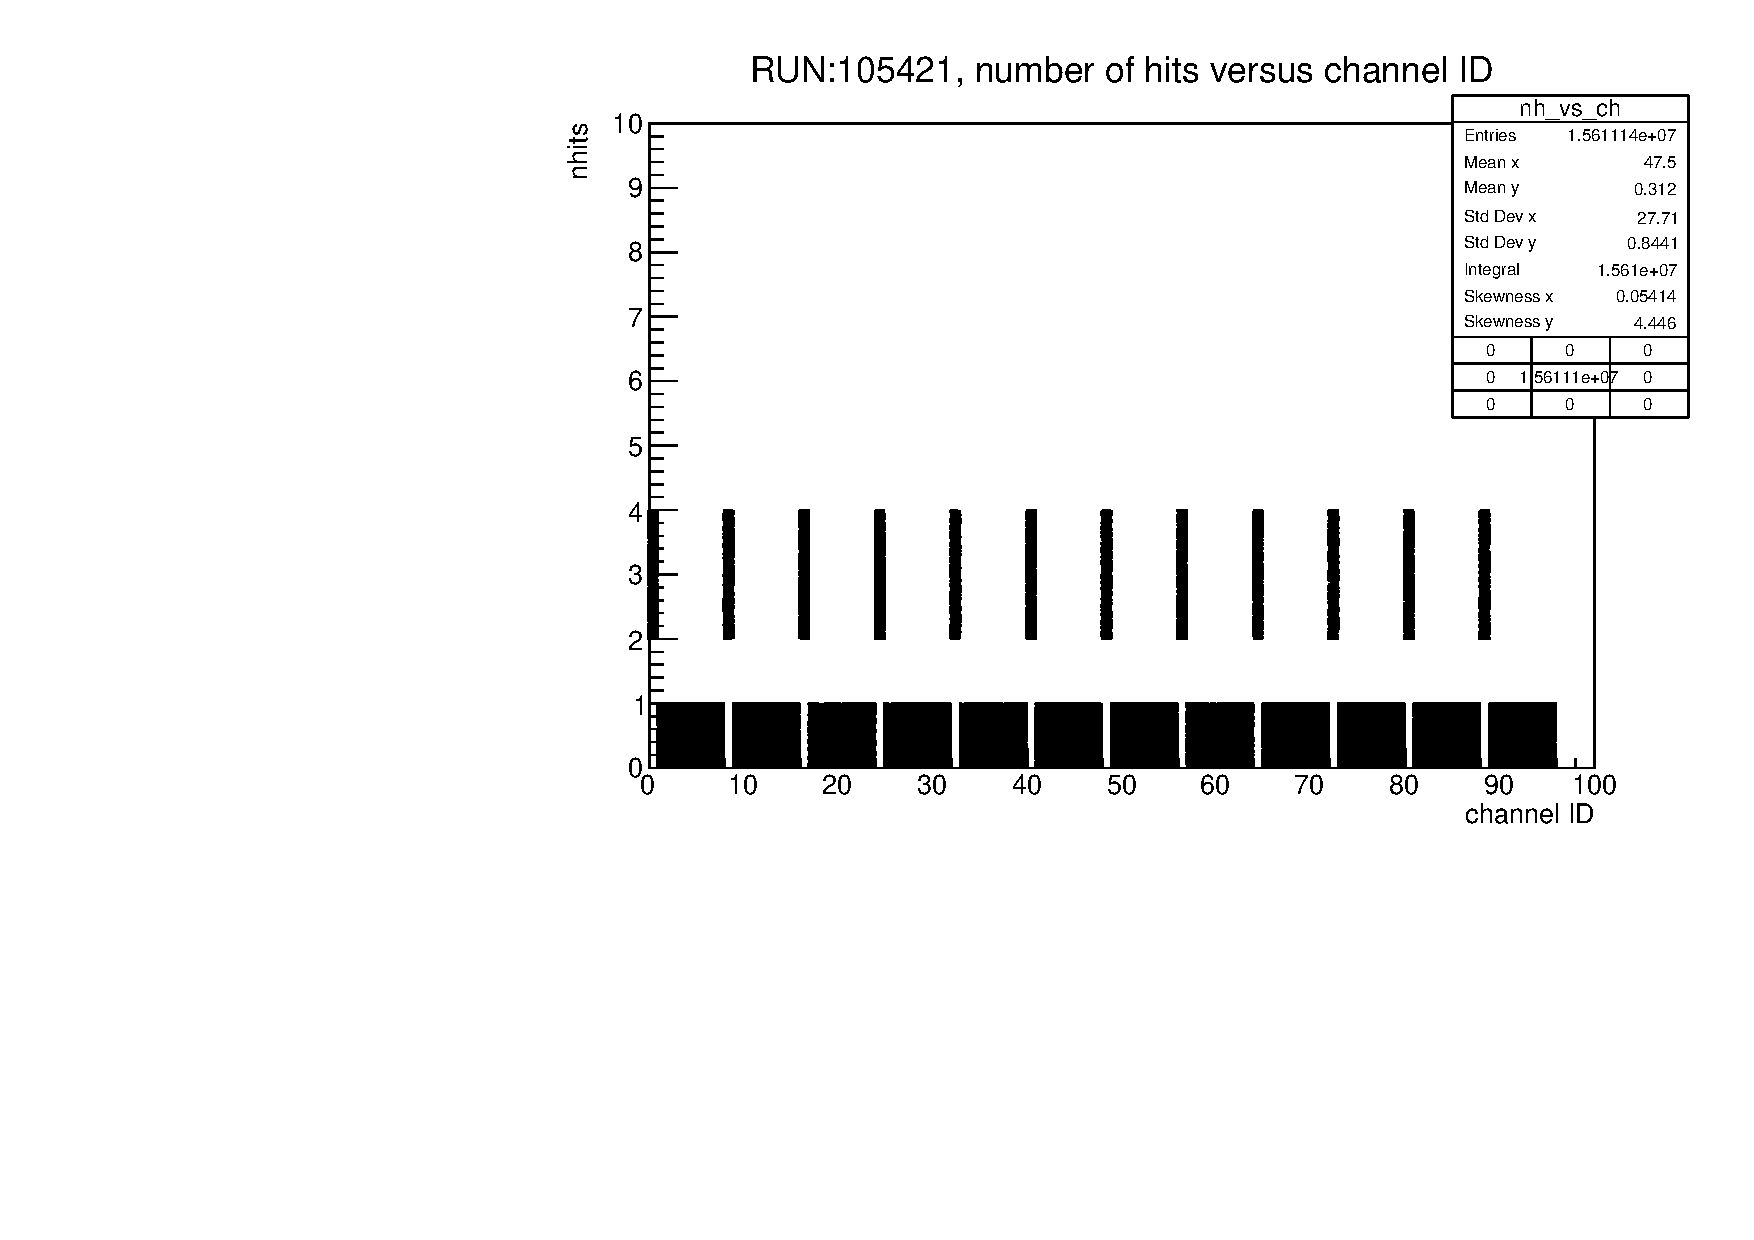
\includegraphics[width=0.95\columnwidth]{figures/pdf/run105421_nh_vs_ch.pdf}
     \label{fig:normalhits}
\end{figure}
\end{column}
\begin{column}{0.5\framewidth}
      \begin{figure}[!h]
      \centering
            \hspace*{-1em}
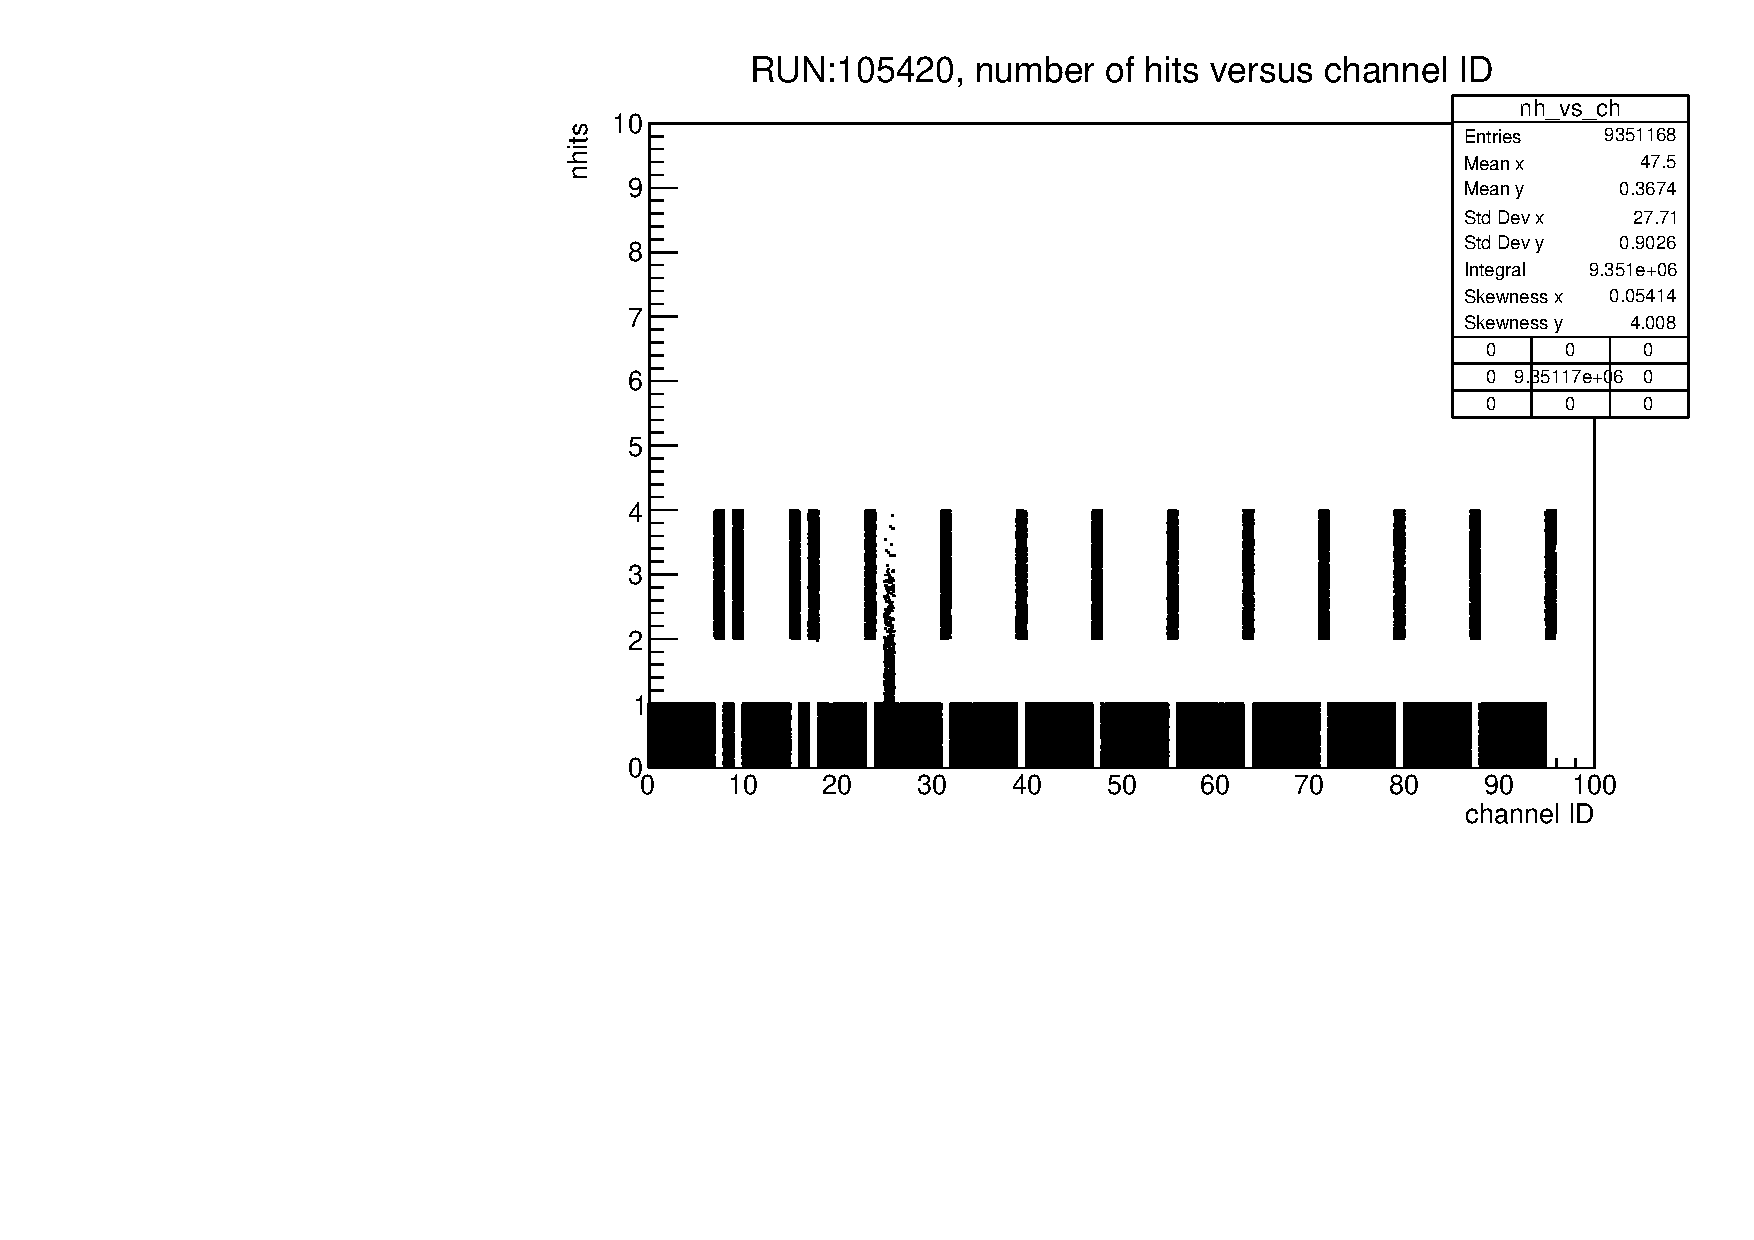
\includegraphics[width=0.95\columnwidth]{figures/pdf/run105420_nh_vs_ch.pdf}
     \label{fig:normalhits}
\end{figure}
\end{column}
\end{columns}
\vspace{-1.5mm}
    \begin{columns}
    \begin{column}{0.63\framewidth}
        \setlength{\leftmargini}{1.1em}
      \begin{itemize}
 {\footnotesize
 \item (Left): regular occupancy;
 \vspace{-0.3mm}
 \item (Top Right): cross talks in first odd \\ channels and only asymmetric \\ (e.g. 3$\rightarrow$5, not seen 3$\rightarrow$1); 
 \vspace{-0.3mm}
 \item (Bottom Right): vertical preamp boards \\ and odd channels on the AMB board;
 \vspace{-0.3mm}
 \item First channels are narrower $\rightarrow$ still \\ object of study.}
\end{itemize}
\end{column}
\begin{column}{0.5\framewidth}
         \begin{figure}[!h]
      \centering
      \hspace*{-2em}
      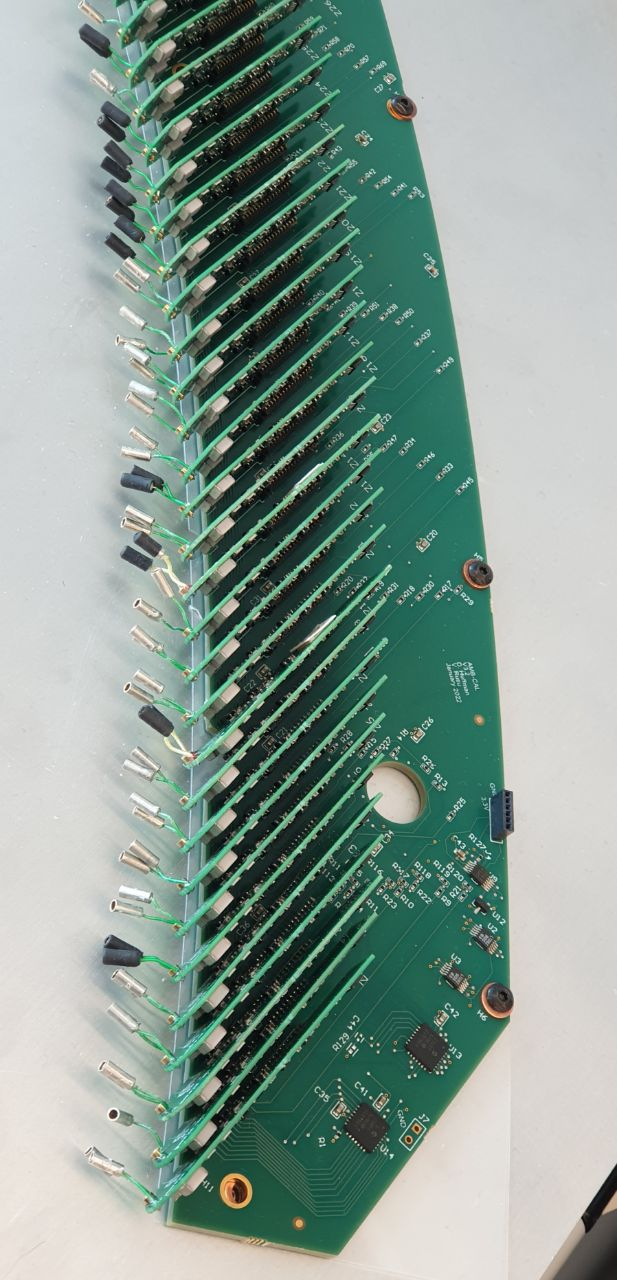
\includegraphics[angle=90,width=1.1\columnwidth]{figures/jpg/photo_6028424923279639562_y.jpg}
     \label{fig:normalhits}
\end{figure}
\end{column}
\end{columns}
\end{frame}















\begin{frame}
    \frametitle{Test 2: analysis of readout waveforms shape}
    \vspace{-4mm}
    \begin{columns}
\begin{column}{1.15\framewidth}
    \setlength{\leftmargini}{1.2em}
 \begin{itemize}
 {\footnotesize
  \item Checking signal uniformity among channels within the same ROC or across multiple ROCs, and among different events;
  \item 40 MHz ADC (25 ns sample width) and pulser frequency set to 50 kHz.}
  \end{itemize}
    \end{column}
    \end{columns}
    \vspace{0mm}
    \begin{columns}
\begin{column}{0.5\framewidth}
         \begin{figure}[!h]
      \centering
      \hspace*{-2em}
      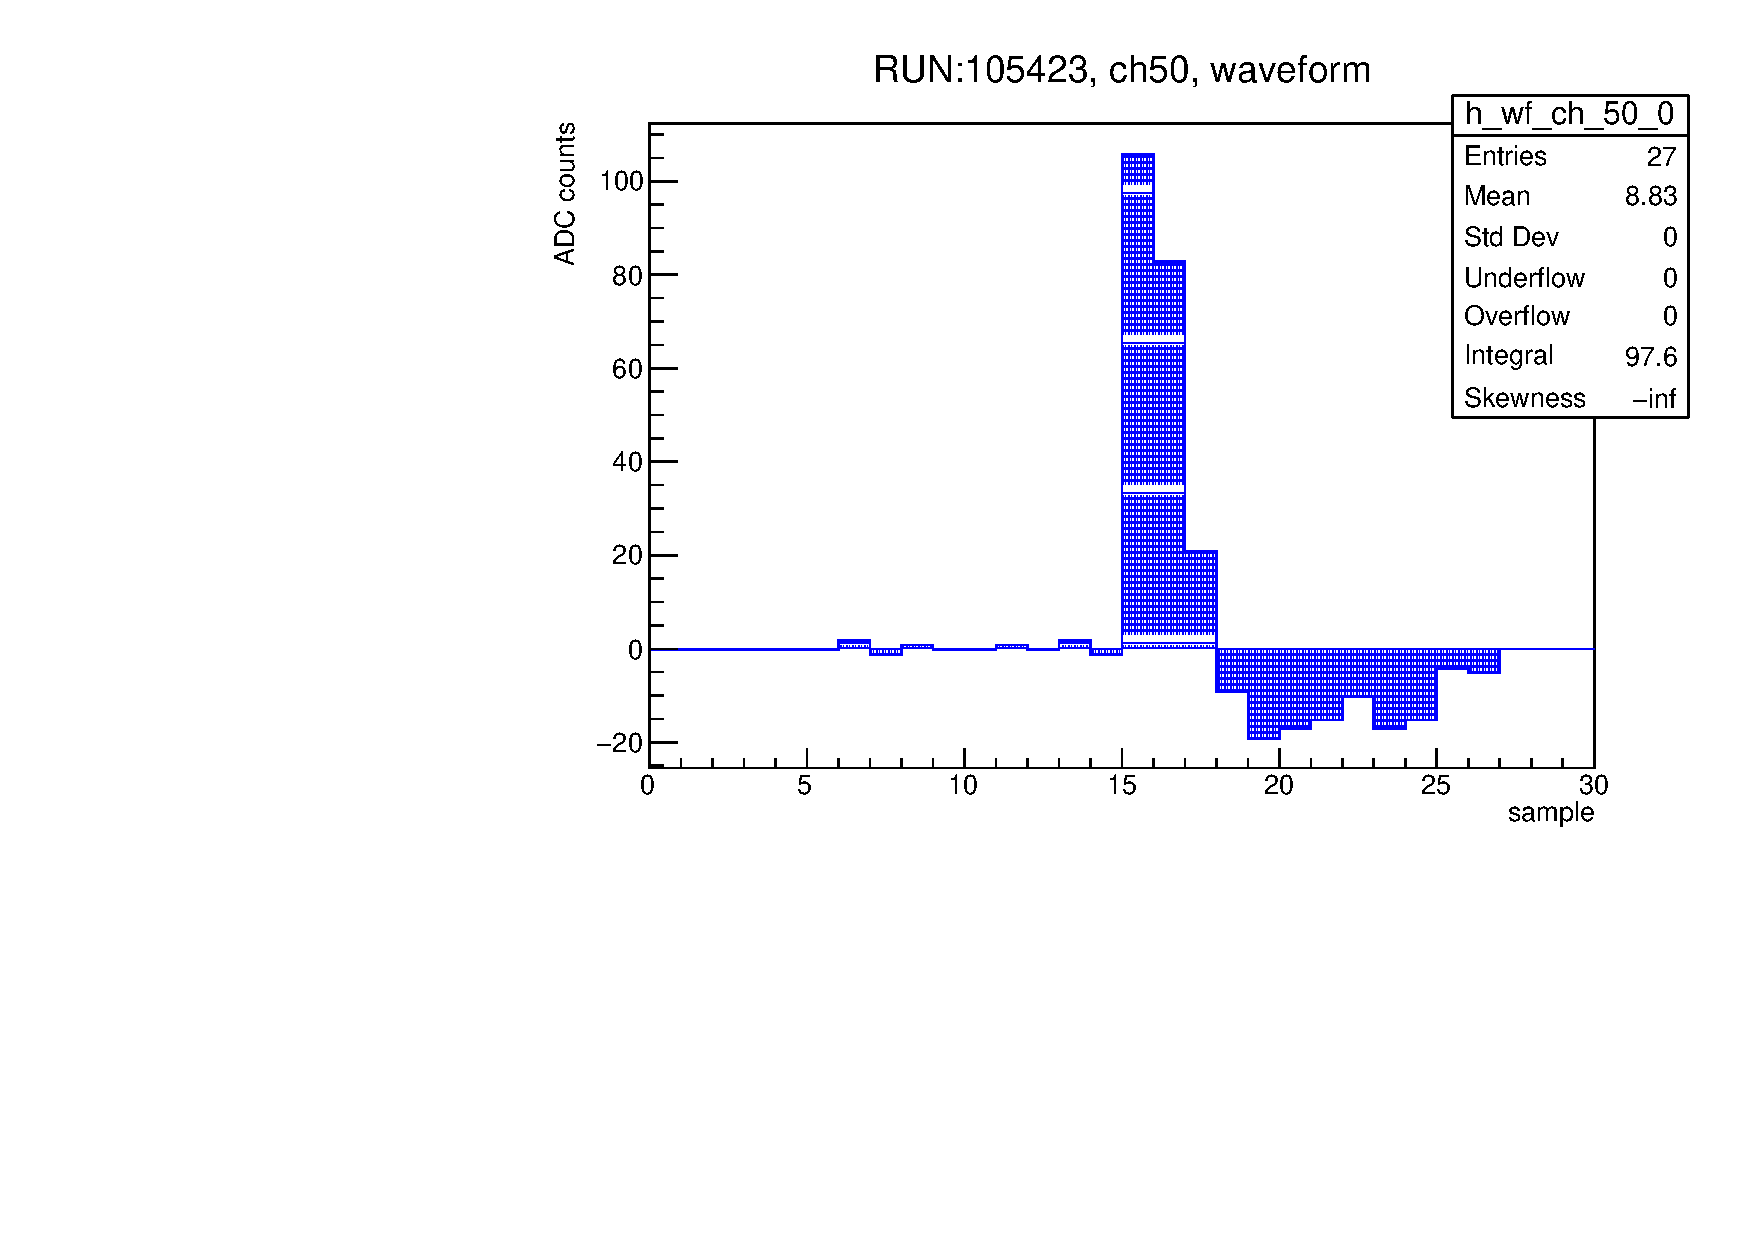
\includegraphics[width=1.\columnwidth]{figures/pdf/wf_ch50_0.pdf}
     \label{fig:normalhits}
\end{figure}
\end{column}
\begin{column}{0.5\framewidth}
      \begin{figure}[!h]
      \centering
            \hspace*{-1em}
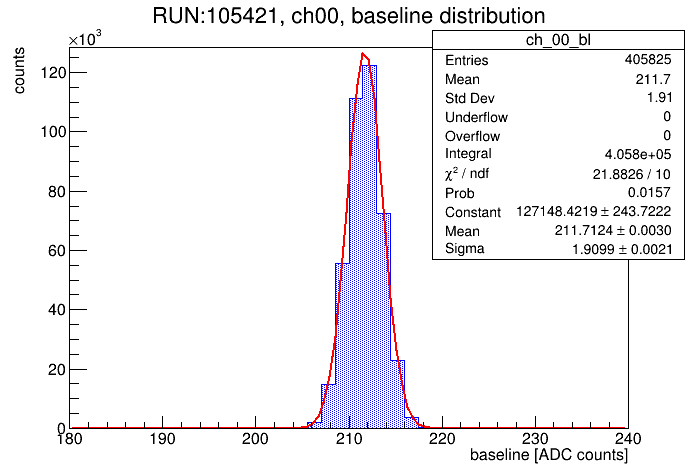
\includegraphics[width=1.\columnwidth]{figures/png/baseline_ch00.png}
     \label{fig:normalhits}
\end{figure}
\end{column}
\end{columns}
\vspace{-1mm}
    \begin{columns}
\begin{column}{1.15\framewidth}
    \setlength{\leftmargini}{1.2em}
 \begin{itemize}
 {\footnotesize
 \item (Left): regular waveform;
\item Flat distribution in the first 10 samples (baseline), high positive charge peak with a sharp leading edge, negative tail;
\item (Right): fitted baseline distibution, with mean at 210 ADC counts and FWHM$=2 \sqrt{2 \text{ln}2}\sigma\sim$4.5 ADC counts. }
\end{itemize}
\end{column}
\end{columns}
\end{frame}

 
\begin{frame}
    \frametitle{Test 2: analysis of readout waveforms shape}
    \vspace{-4mm}
    \begin{columns}
\begin{column}{1.15\framewidth}
    \setlength{\leftmargini}{1.2em}
 \begin{itemize}
{\footnotesize \item Different baseline values indicating noise and inverted waveforms.}
  \end{itemize}
    \end{column}
    \end{columns}
        \vspace{-3mm}
    \begin{columns}
\begin{column}{0.5\framewidth}
         \begin{figure}[!h]
      \centering
      \hspace*{-2em}
      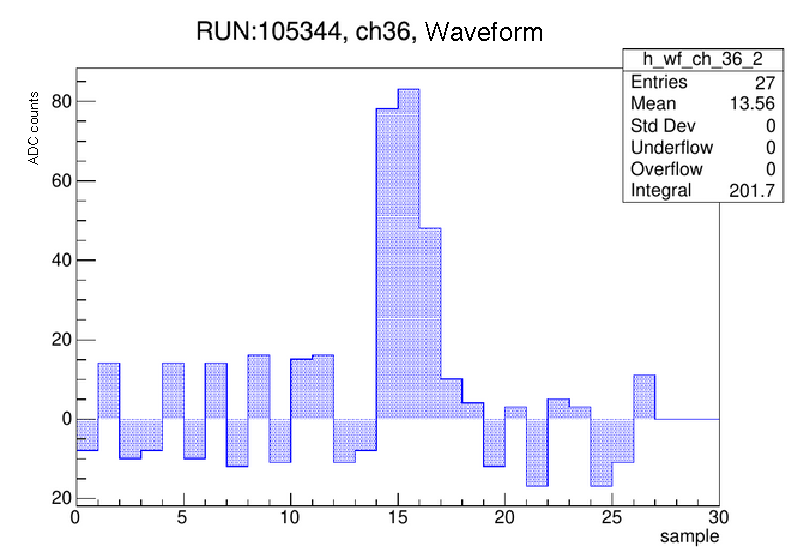
\includegraphics[width=\columnwidth]{figures/pdf/noise.pdf}
     \label{fig:normalhits}
\end{figure}
\end{column}
\begin{column}{0.5\framewidth}
      \begin{figure}[!h]
      \centering
            \hspace*{-1em}
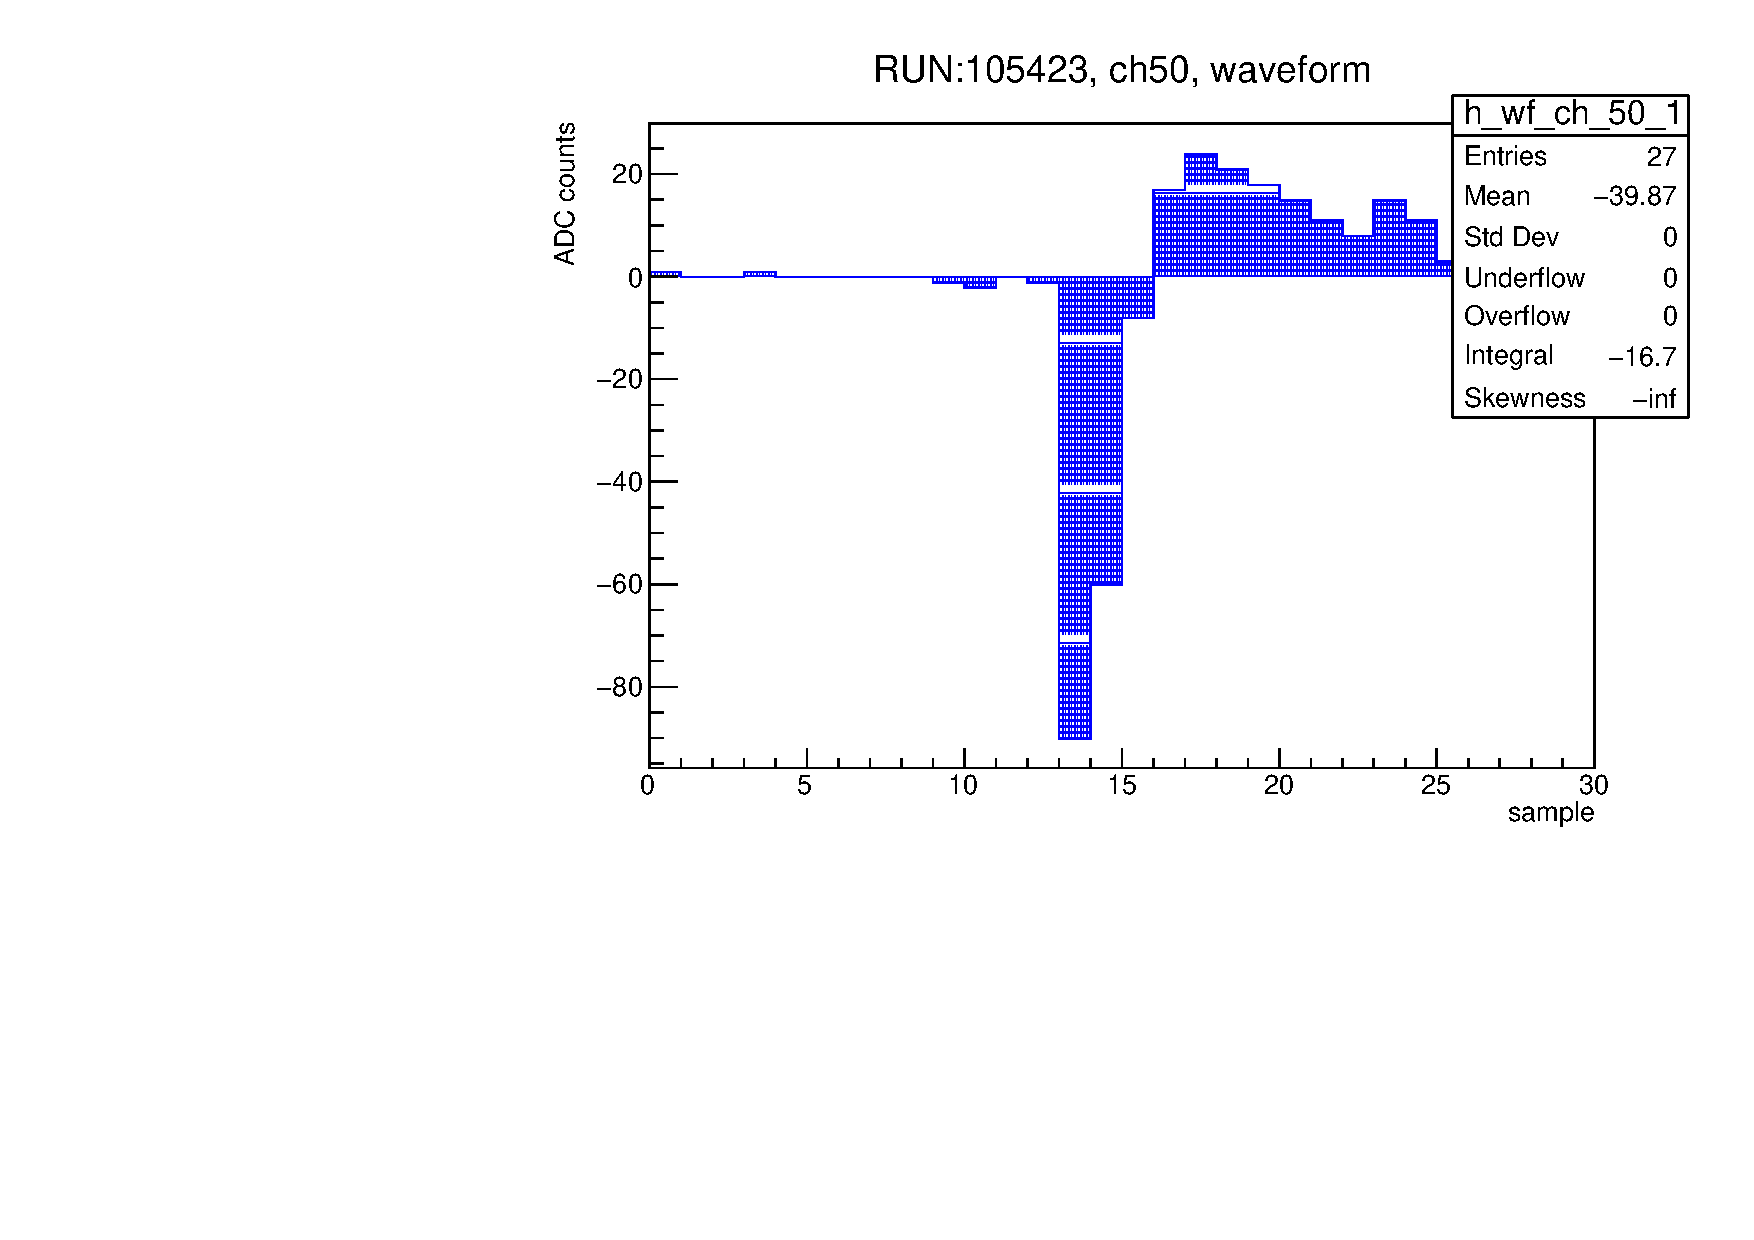
\includegraphics[width=\columnwidth]{figures/pdf/wf_ch50_1.pdf}
     \label{fig:normalhits}
\end{figure}
\end{column}
\end{columns}
    \begin{columns}
    \begin{column}{0.63\framewidth}
        \setlength{\leftmargini}{1.1em}
      \begin{itemize}
 {\footnotesize
 \item (Left): noisy waveform;
\item (Right): inverted waveform $\rightarrow \Delta t $ distribution peaked in 16 $\mu$s (regular) \\ and 4 $\mu$s (inverted). Trigger on trailing \\ edge of 4 $\mu$s long input pulses;
\item Occupancy distribution with $N_{hits}> 3$ per channel (preamp substituted).}

\end{itemize}
\end{column}
\begin{column}{0.5\framewidth}
         \begin{figure}[!h]
      \centering
      \hspace*{-2em}
      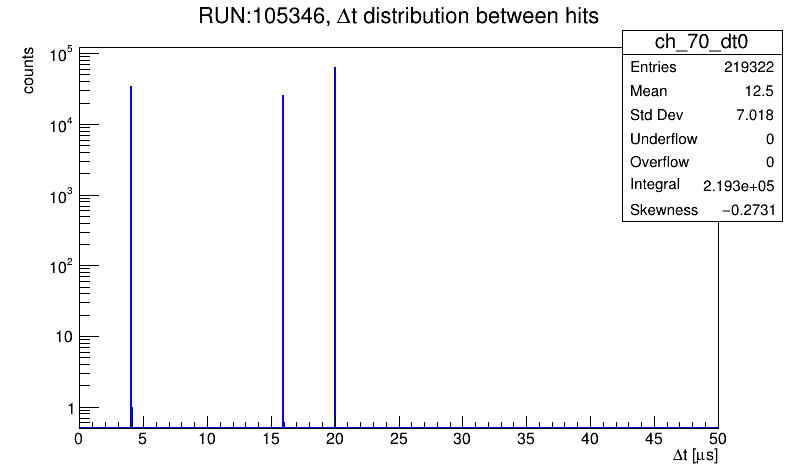
\includegraphics[width=\columnwidth]{figures/png/deltathits.png}
     \label{fig:normalhits}
\end{figure}
\end{column}
\end{columns}
\end{frame}


\begin{frame}
    \frametitle{Test 2: analysis of readout waveforms shape}
    \vspace{-3mm}
    \begin{columns}
\begin{column}{1.15\framewidth}
    \setlength{\leftmargini}{1.2em}
 \begin{itemize}
{\footnotesize \item (Left): pulse height (PH) (charge) distribution with 2/3 peaks.}
  \end{itemize}
    \end{column}
    \end{columns}
        \vspace{-2mm}
    \begin{columns}
\begin{column}{0.5\framewidth}
         \begin{figure}[!h]
      \centering
      \hspace*{-2em}
      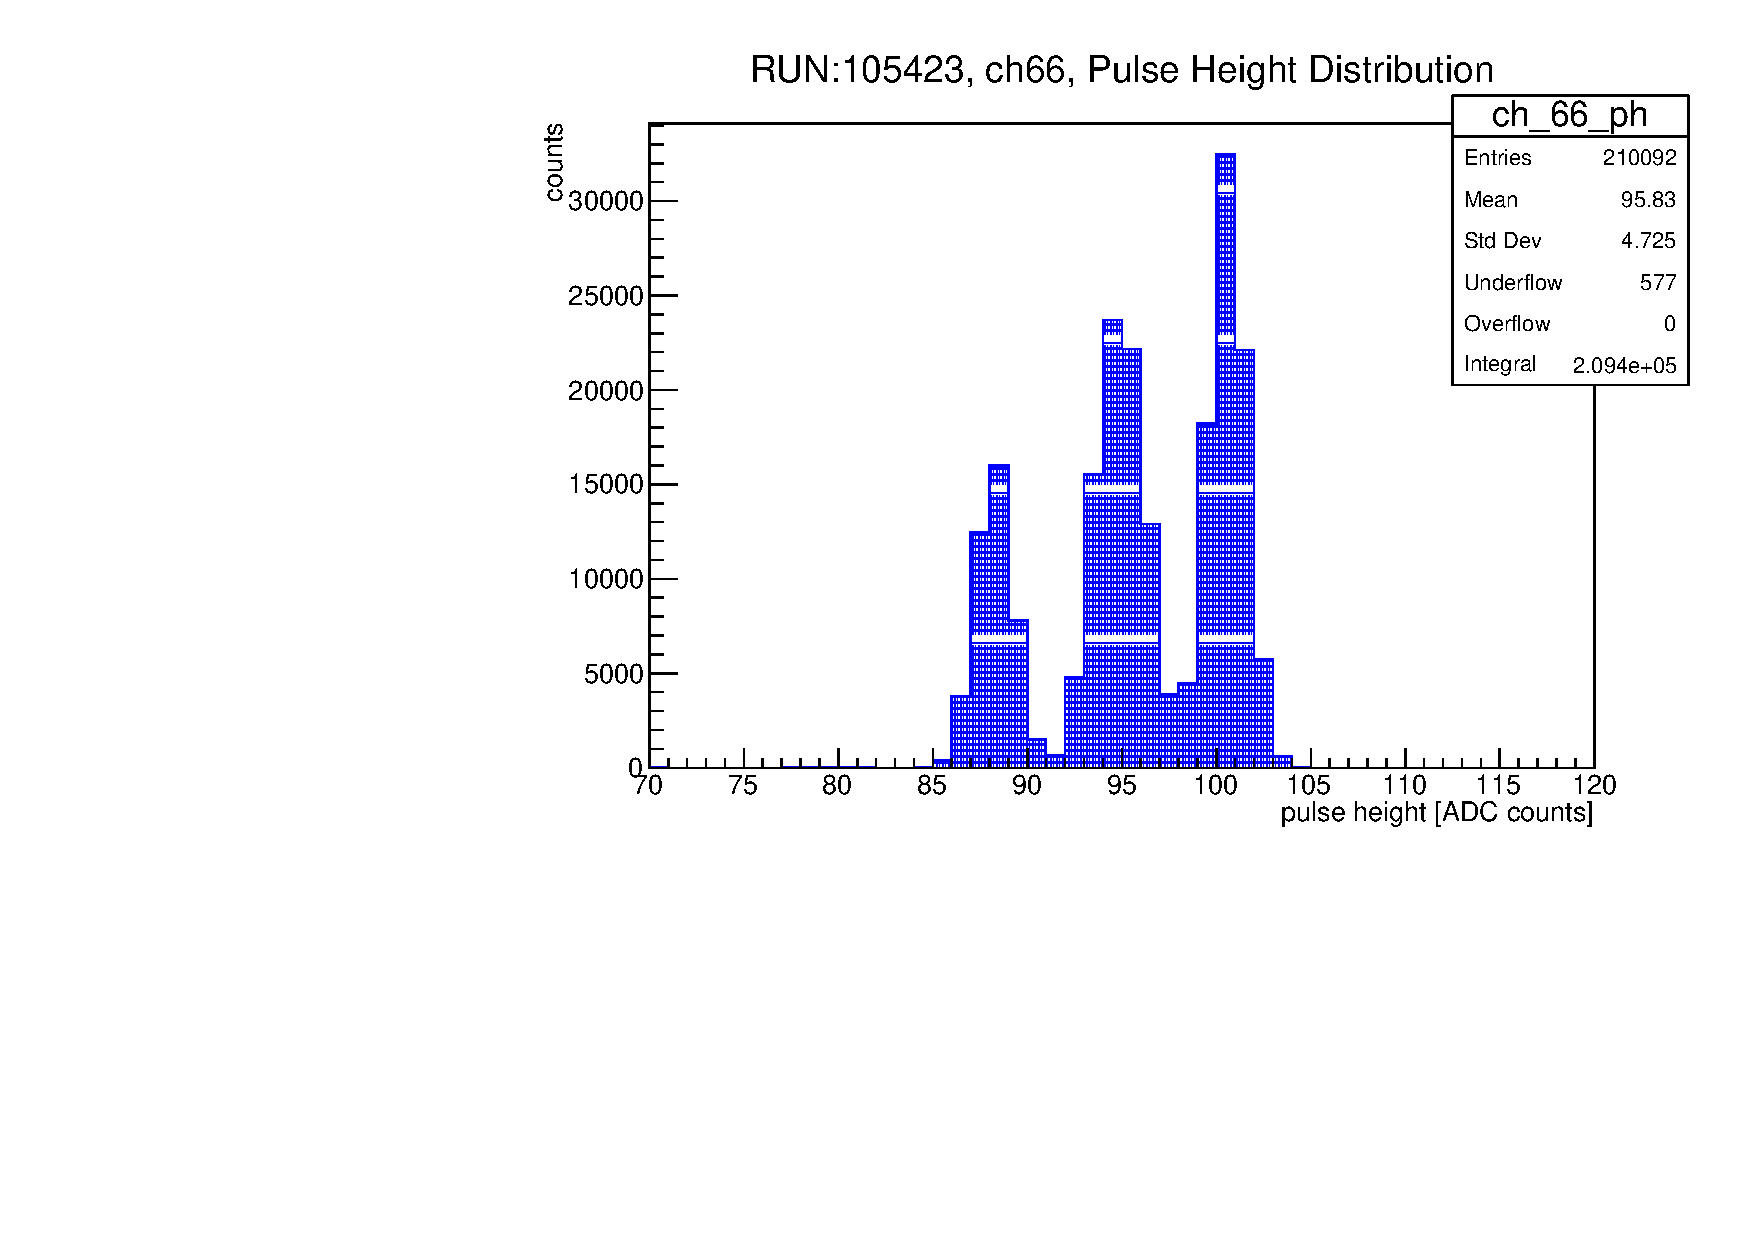
\includegraphics[width=0.9\columnwidth]{figures/pdf/pulseheight.pdf}
     \label{fig:normalhits}
\end{figure}
\end{column}
\begin{column}{0.5\framewidth}
      \begin{figure}[!h]
      \centering
            \hspace*{-1em}
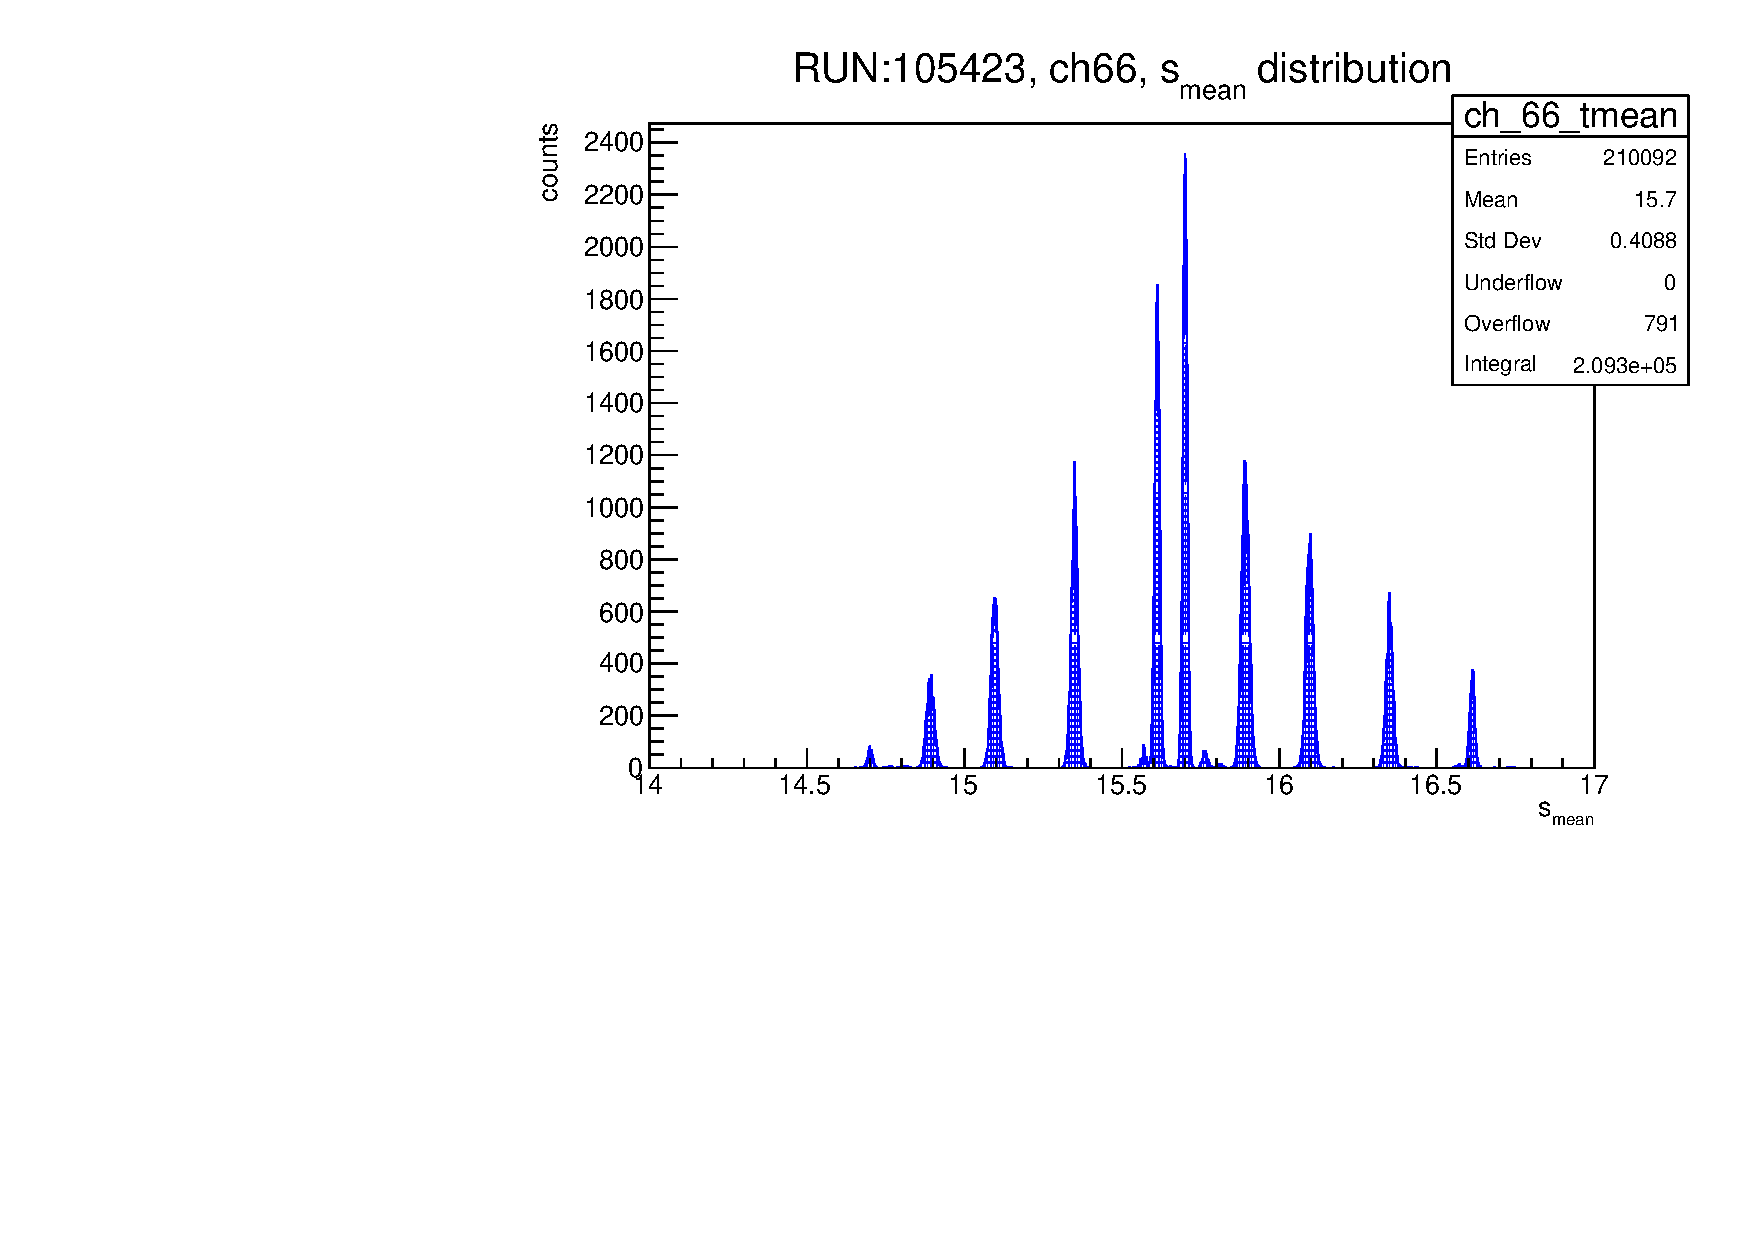
\includegraphics[width=0.9\columnwidth]{figures/pdf/tmean1.pdf}
     \label{fig:normalhits}
\end{figure}
\end{column}
\end{columns}
\vspace{-5mm}
    \begin{columns}
    \begin{column}{0.55\framewidth}
        \setlength{\leftmargini}{1.em}
      \begin{itemize}
 {\footnotesize
\item (Top Right): $s_{mean} = \frac{\sum_i \text{sample}_i \cdot q_i }{\sum_i q_i} $ distribution, correlated with PH (charge) peaks;
\item (Bottom Right): simulation of the charge and PH distribution \\ behaviour;
\item This is an artifact of the pulser \\
timing shifted with respect to the \\ ADC 
clock of few ns.}

\end{itemize}
\end{column}
\begin{column}{0.55\framewidth}
         \begin{figure}[!h]
      \centering
      \hspace*{-2em}
      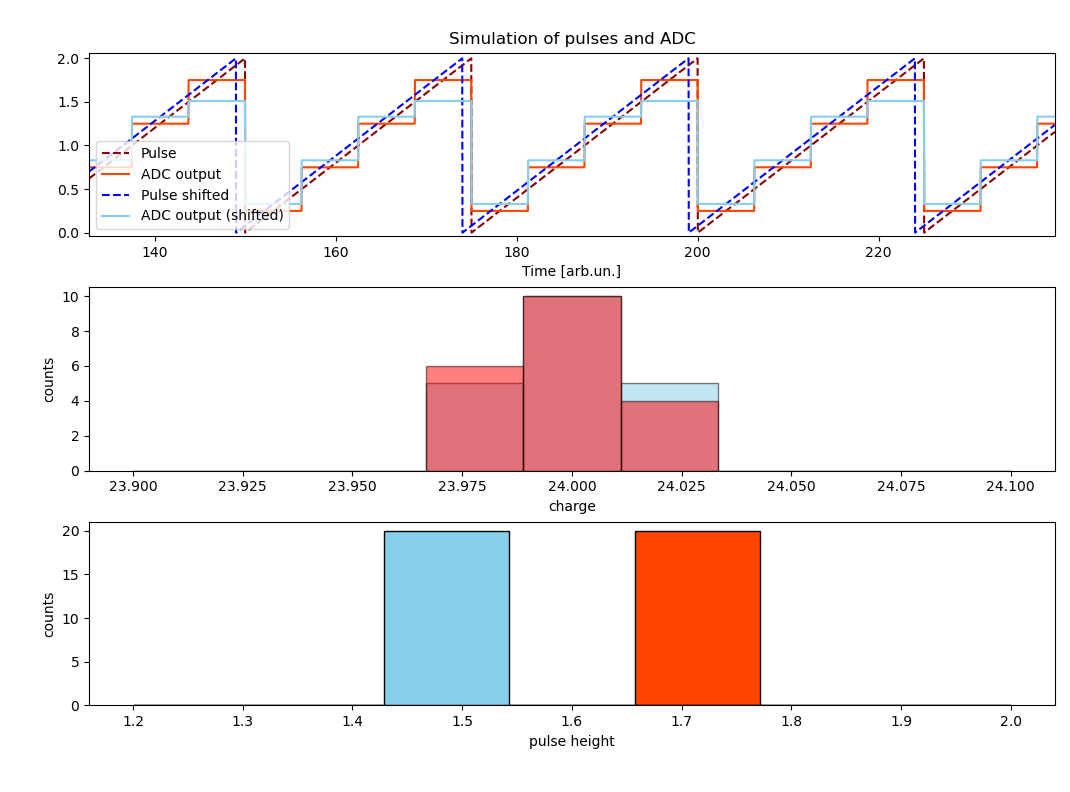
\includegraphics[width=1.05\columnwidth]{figures/png/pres.png}
     \label{fig:normalhits}
\end{figure}
\end{column}
\end{columns}
\end{frame}




\begin{frame}
    \frametitle{Outline}
    
\begin{itemize}
\item \textcolor{mygray}{Commissioning of the tracker DAQ and FEE:}
\begin{itemize}
         \vspace{2mm}

    \item \textcolor{mygray}{validation of ROC readout;}
             \vspace{1.5mm}

    \item \textcolor{mygray}{study of preamplifiers performance}.
\end{itemize}
\vspace{4mm}
    \item First steps towards the station calibration;
    \vspace{6mm}

    \item \textcolor{mygray}{Pre-pattern recognition studies;}
  \vspace{6mm}
    \item \textcolor{mygray}{Conclusions.}
\end{itemize}
\end{frame}

\begin{frame}
    \frametitle{First steps towards the station calibration}
    
      \begin{columns}
        \begin{column}{0.65\framewidth}
                \setlength{\leftmargini}{1.2em}
                \vspace{-7mm}
            \begin{itemize}
             {\footnotesize 
             \item \textbf{Calibration goal}: straw longitudinal position resolution $\lesssim$4 cm with cosmics;
           \vspace{4mm}
             \item TDCs measure arrival times $t_1$ and $t_2$;
             \vspace{4mm}
             \item $x_{track}$: information about the hit straws $\rightarrow$ \textbf{station geometry};   
  \vspace{4mm}
                \item \textbf{Calibration}: from $\Delta t_{12}$ and $x_{\text{track}}$ $\rightarrow$ $v$ (signal propagation velocity);                  
              \vspace{4mm}
                \item $Horizontal$ $\rightarrow$ unbiased reconstruction; 
                               \vspace{4mm}
                \item Operational constraints ($vertical$);
                  \vspace{4mm}
                \item \textbf{Simulation with vertical station to assess biases and feasibility}.}  
            \end{itemize}
        \end{column}
        \begin{column}{0.48\framewidth}
            \begin{equation*}
\begin{aligned}
    t_1 &= t_0 + t_d + \frac{x_{\text{track}}}{v}  + d_1 \\
    t_2 &= t_0 + t_d + \frac{L - x_{\text{track}}}{v}  + d_2 \\
    \Delta & t_{12} = \frac{2x_{\text{track}}-L}{v} +(d_1-d_2)
\end{aligned}
\end{equation*}

\begin{figure}[!h]
\centering
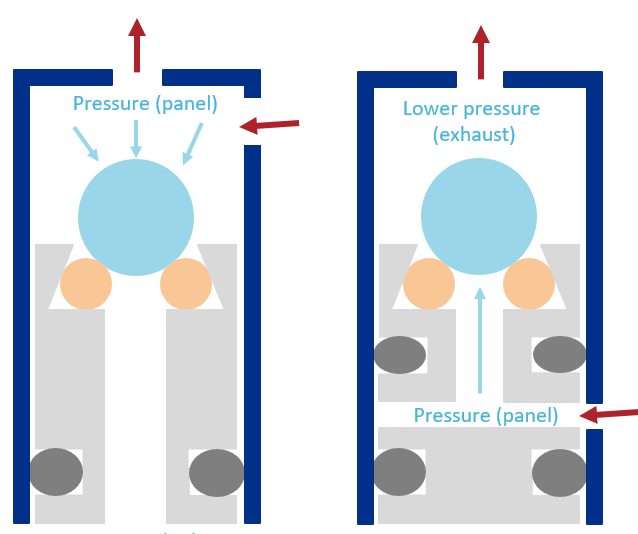
\includegraphics[width =\columnwidth]{figures/png/gassystem.png}
\label{fig:gassystem}
\end{figure}
        \end{column}
    \end{columns}
  
\end{frame}


\begin{frame}
    \frametitle{Monte Carlo muon selection and reconstruction}
\vspace{-4.6mm}
    \begin{columns}
\begin{column}{0.65\framewidth}
   \setlength{\leftmargini}{1.2em}
   \begin{itemize}
{\footnotesize \item \textbf{Straw information}:}
\vspace{2mm}
\begin{itemize}
    {\footnotesize \item the direction $(D_{x,i},D_{y,i})$;
    \vspace{1mm}
    \item the midpoint $(M_{x,i},M_{y,i})$;
    \vspace{1mm}
    \item the $z_i$ coordinate.}
\end{itemize} 
\vspace{4mm}
 {\footnotesize
 \item \textbf{Selection}:}
 \vspace{2mm}
  \begin{itemize}
   {\footnotesize 
    \item \textbf{Straight line in 3D}: $\geq$4 hits at different $z$ $\rightarrow$ $nhits_{face_i}\geq 1$;
    \vspace{1mm}
    \item \textbf{Resolution}: $nhits_{panel_i}\leq 3$.}
    \end{itemize} 
    \vspace{4mm}
 {\footnotesize \item \textbf{Reconstruction}: }
 \vspace{2mm}
        \begin{itemize}
        {\footnotesize \item $StrawHit$s $\rightarrow$ 1 $ClusterHit$ (face);
        \vspace{1mm}
          \item 2 $ClusterHit$s $\rightarrow$ $StereoHit$ (plane);
          \vspace{1mm}
          \item 2 $StereoHit$s $\rightarrow$ reconstructed track.}
        \end{itemize}

\end{itemize}
\end{column}
\begin{column}{0.5\framewidth}
      \begin{figure}[!h]
      \centering
            \hspace*{-2em}
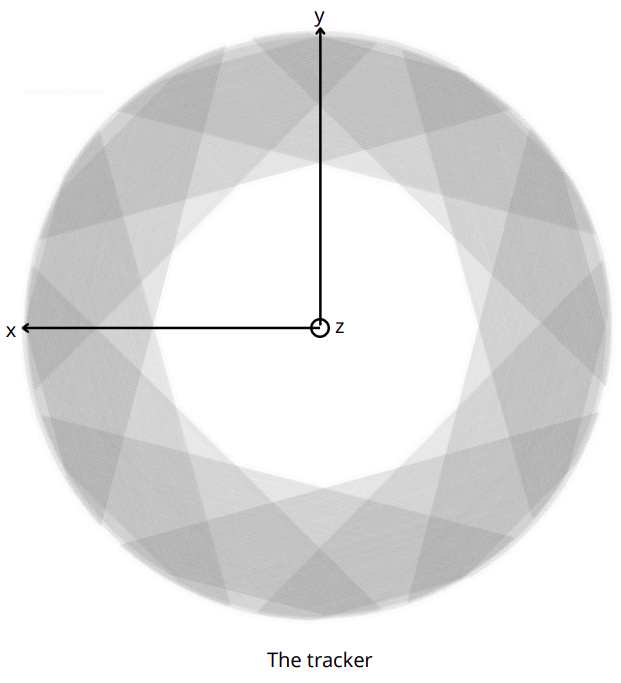
\includegraphics[width=0.7\columnwidth]{figures/png/Screenshot_20240526_164527.png}
     \label{fig:normalhits}
\end{figure}
\vspace{-5mm}
         \begin{figure}[!h]
      \centering
      \hspace*{-2em}
      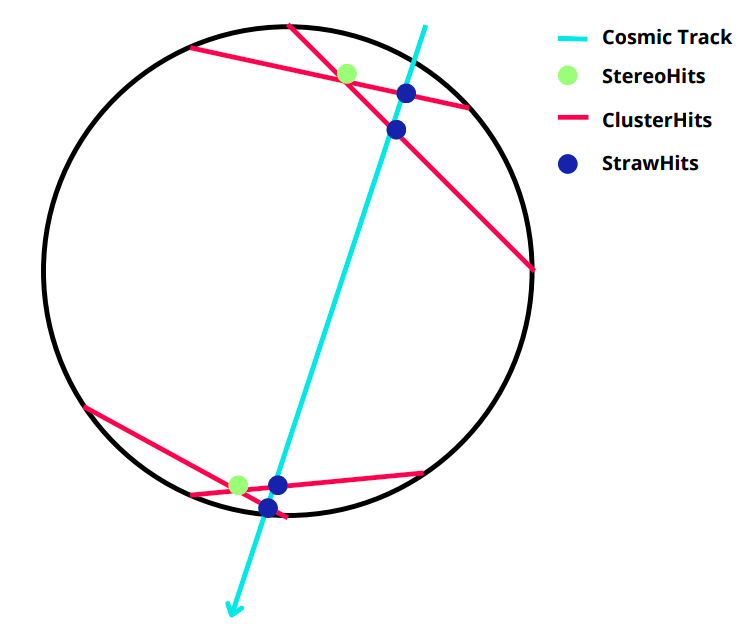
\includegraphics[width=0.9\columnwidth]{figures/png/Screenshot_20240810_210144.png}
     \label{fig:normalhits}
\end{figure}
\end{column}
\end{columns}
\end{frame}




\begin{frame}
    \frametitle{Panel illumination pattern and muon directions}
    \begin{columns}
\begin{column}{0.65\framewidth}
\vspace{-8mm}
   \setlength{\leftmargini}{1.2em}
      \begin{itemize}
 {\footnotesize
 
\item (Top): muon selection $\rightarrow$ \textbf{non uniform} \\ panel illumination;
 \vspace{6mm}
\item 4/4 overlap areas limited to \textbf{panel edges};
 \vspace{6mm}
\item \textbf{Time walk effects};
 \vspace{6mm}
\item (Bottom): $m_{yz}=\Delta y /\Delta z$ distribution;
 \vspace{6mm}
 \item Selection of \textbf{specific muon directions};
 \vspace{6mm}
\item Mostly with $|m_{yz}| \sim 1$ (\textbf{45° angle});
 \vspace{6mm}
\item Muon \textbf{rate} scaled.}

\end{itemize}
\end{column}
\begin{column}{0.5\framewidth}
\vspace{-2mm}
      \begin{figure}[!h]
      \centering
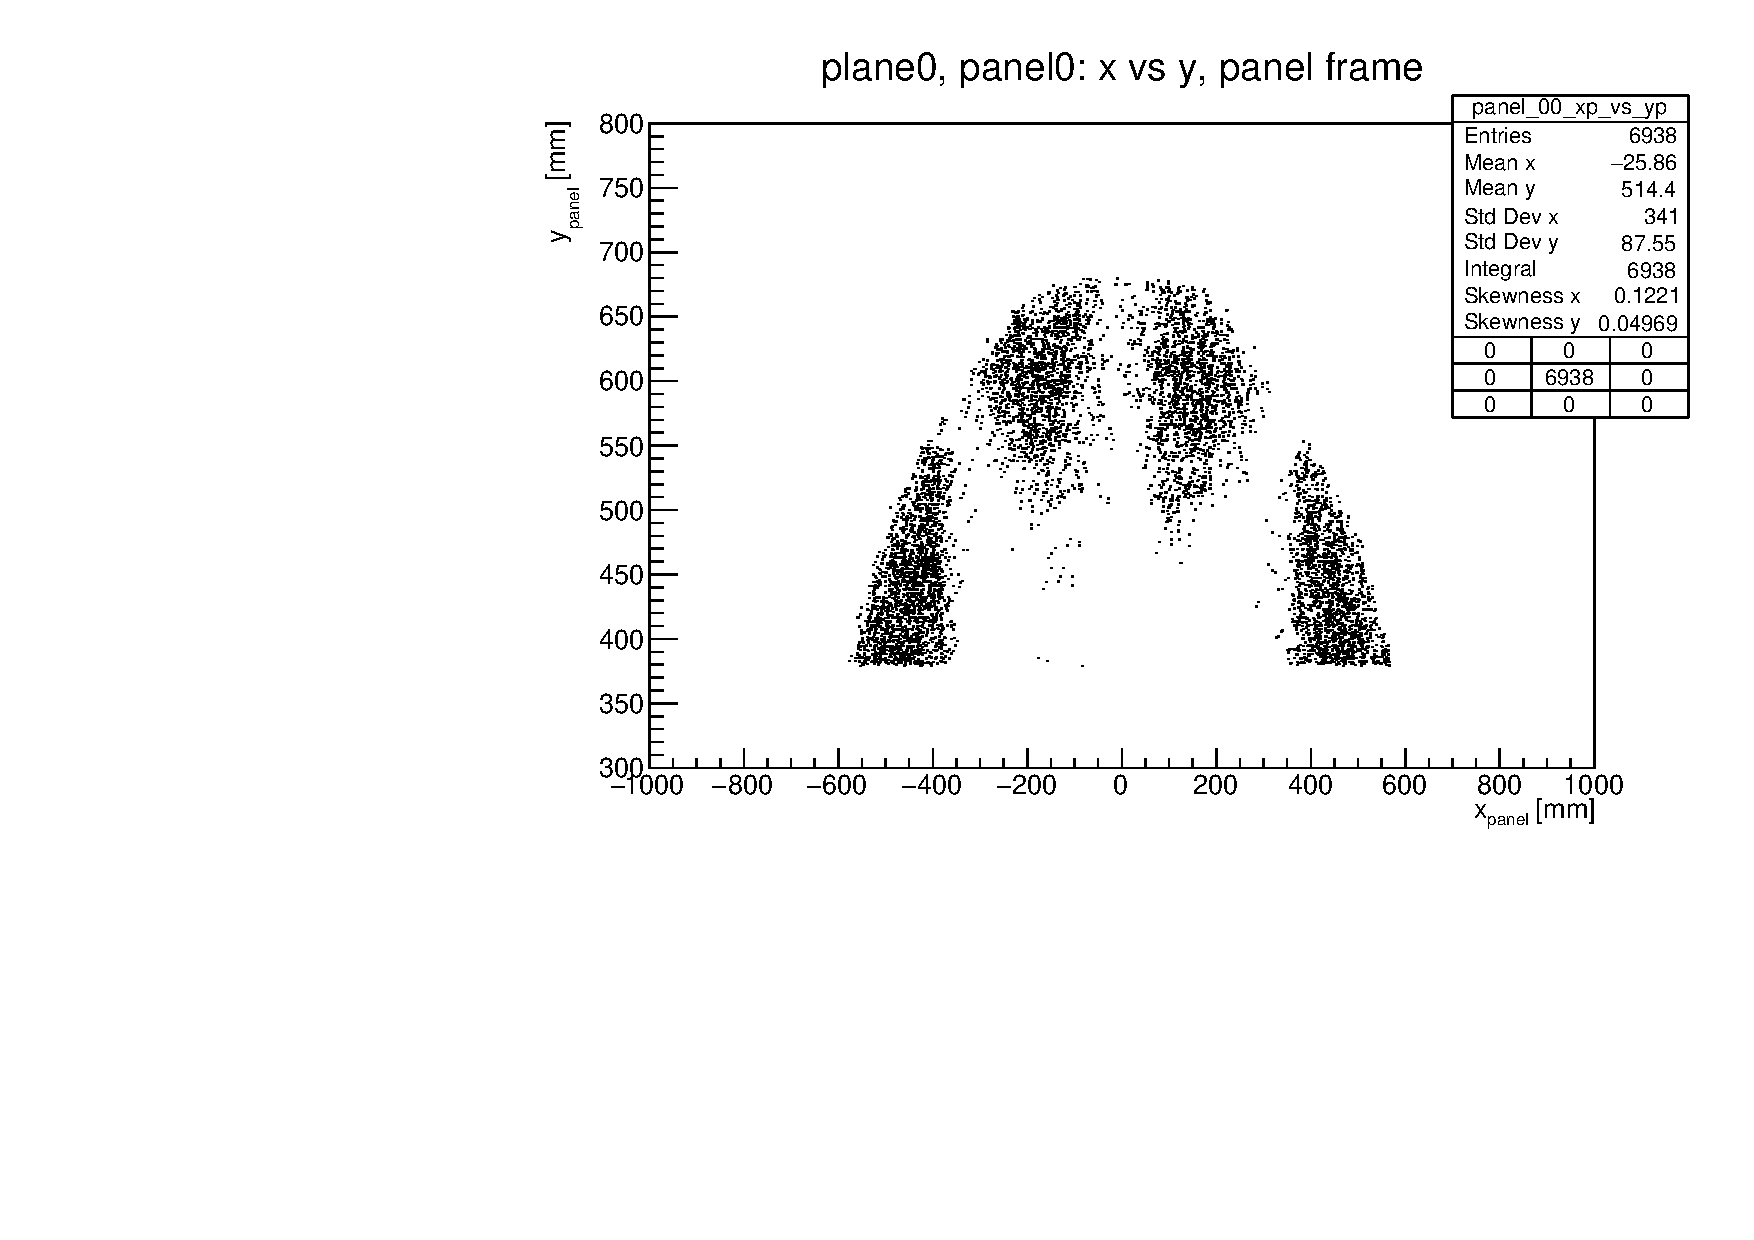
\includegraphics[width=1.\columnwidth]{figures/pdf/xp_vs_yp_panel0.pdf}
     \label{fig:normalhits}
\end{figure}
\vspace{-5mm}
         \begin{figure}[!h]
      \centering
      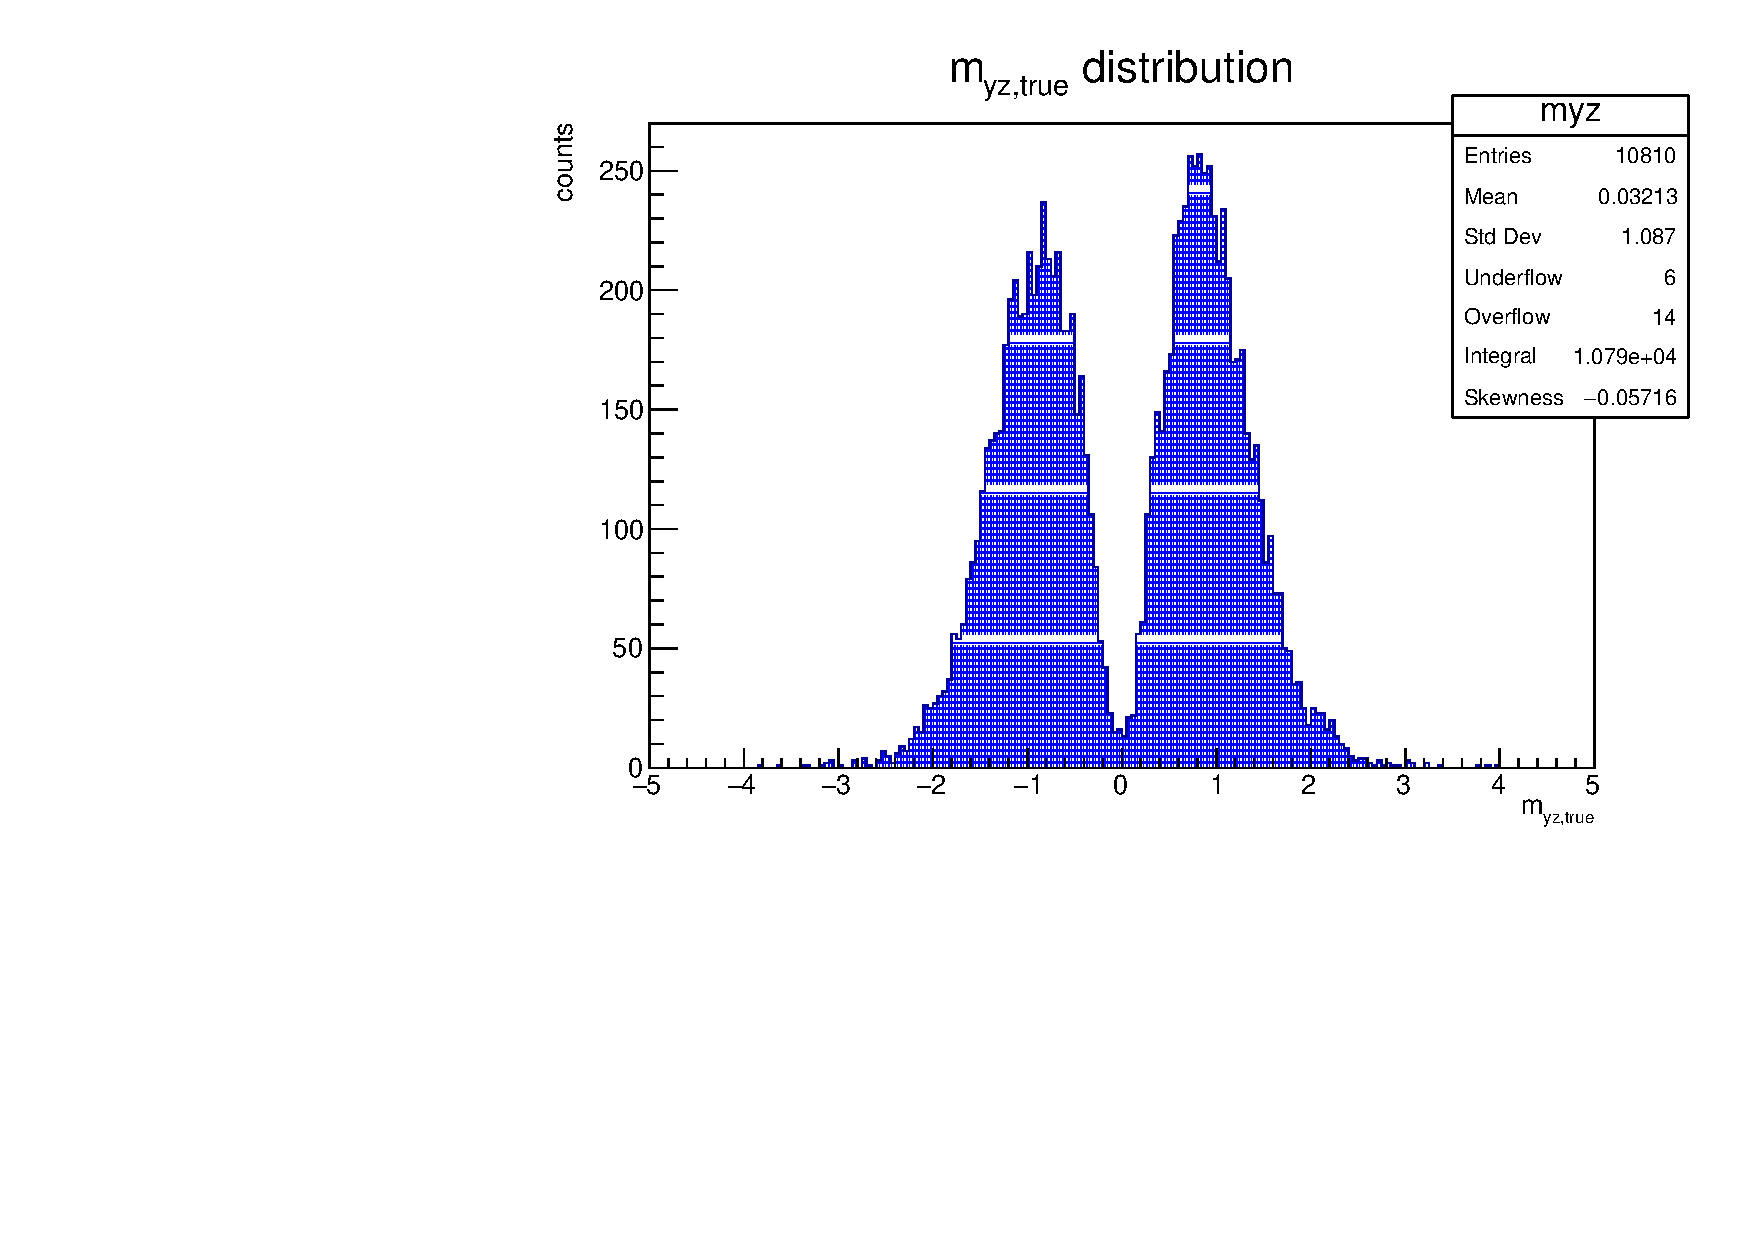
\includegraphics[width=1.\columnwidth]{figures/pdf/myz.pdf}
     \label{fig:normalhits}
\end{figure}
\end{column}
\end{columns}
\end{frame}













\begin{frame}
    \frametitle{Longitudinal position reconstruction}

    \begin{columns}
\begin{column}{0.65\framewidth}
\vspace{-6mm}
   \setlength{\leftmargini}{1.2em}
      \begin{itemize}
 {\footnotesize
 \item (Top): \textbf{longitudinal reconstructed position} $x_{track}$ (panel frame);
 \vspace{5mm}
 \item $x_{track}$: reconstructed track and panel $z_i$ intersection;
 \vspace{5mm}
 \item  \textbf{Bumps} $\rightarrow$ 4/4 requirement consequence;
 \vspace{5mm}
\item Different bumps $\rightarrow$ different straws;
\vspace{5mm}
\item (Bottom): $\Delta x = x_{track}-x_{true}$ distribution;
  \vspace{5mm}
\item The bias ranges between [-6,6] cm;
  \vspace{5mm}
\item $m_{yz}=\Delta y/\Delta z$ not accurately reconstructed.}

\end{itemize}
\end{column}
\begin{column}{0.5\framewidth}
\vspace{-3mm}
      \begin{figure}[!h]
      \centering
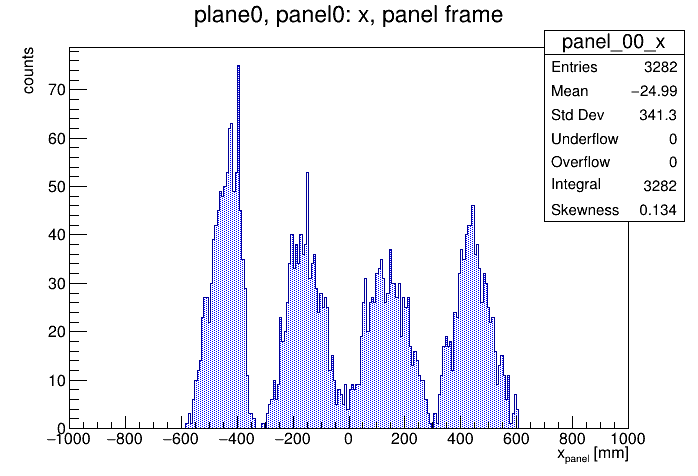
\includegraphics[width=1.\columnwidth]{figures/png/x_panel0.png}
     \label{fig:normalhits}
\end{figure}
\vspace{-5mm}
         \begin{figure}[!h]
      \centering
      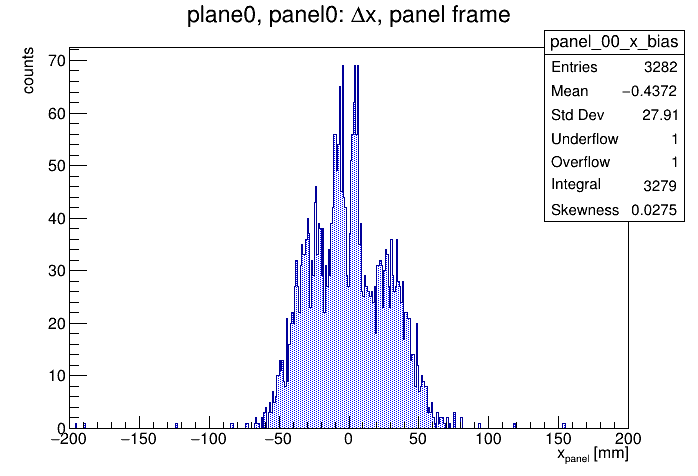
\includegraphics[width=1.\columnwidth]{figures/png/panel_00_x_bias.png}
     \label{fig:normalhits}
\end{figure}
\end{column}
\end{columns}
\end{frame}






\begin{frame}
    \frametitle{Results}

    \begin{columns}
\begin{column}{0.65\framewidth}
\vspace{-8mm}
   \setlength{\leftmargini}{1.2em}
      \begin{itemize}
 {\footnotesize
    \item (Top): 2D distribution of $\Delta x$ vs $x_{true}$;
    \vspace{4mm}
    \item Different \textbf{spots} $\rightarrow$ different overlap regions and muon directions;
    \vspace{4mm}
    \item (Bottom): $\Delta x$ profile vs $x_{true}$;
    \vspace{4mm}
    \item $x_{track}$ reconstruction \textbf{systematics} $\pm$4 cm;
    \vspace{4mm}
    \item Vertical station: opposite $y-z$ orientated muons do not cancel out;
    \vspace{4mm}
        \item First spots: 90° panels overlap;
        \vspace{4mm}
    \item \textbf{Increase of data-taking time};
    \vspace{4mm}
\item \textbf{Calibration expected to be challenging}. 
}

\end{itemize}
\end{column}
\begin{column}{0.5\framewidth}
\vspace{-3mm}
      \begin{figure}[!h]
      \centering
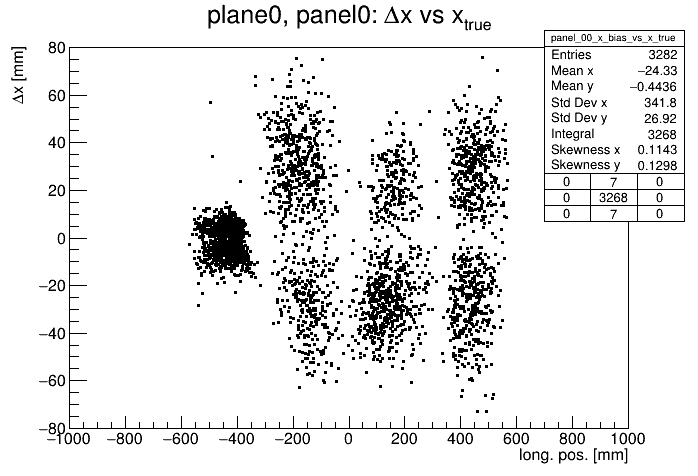
\includegraphics[width=1.\columnwidth]{figures/png/panel_00_x_bias_vs_x.png}
     \label{fig:normalhits}
\end{figure}
\vspace{-5mm}
         \begin{figure}[!h]
      \centering
      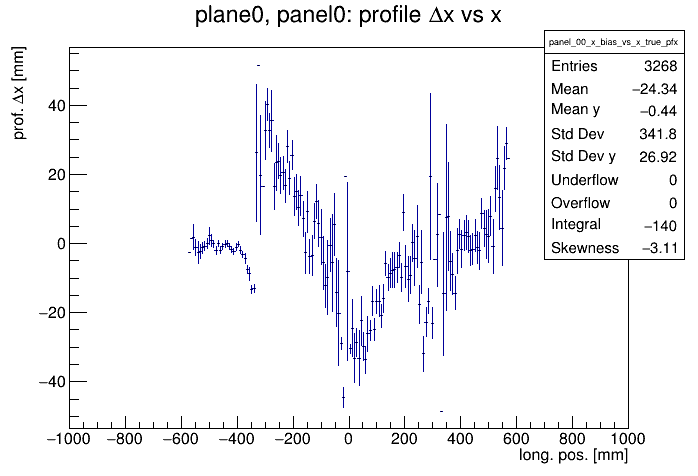
\includegraphics[width=1.\columnwidth]{figures/png/panel_00_x_bias_vs_x_prof.png}
     \label{fig:normalhits}
\end{figure}
\end{column}
\end{columns}
\end{frame}







\begin{frame}
    \frametitle{Outline}
    
\begin{itemize}
\item \textcolor{mygray}{Commissioning of the tracker DAQ and FEE:}
\begin{itemize}
         \vspace{2mm}

    \item \textcolor{mygray}{validation of ROC readout;}
             \vspace{1.5mm}

    \item \textcolor{mygray}{study of preamplifiers performance}.
\end{itemize}
\vspace{4mm}
    \item \textcolor{mygray}{First steps towards the station calibration;}
    \vspace{6mm}

    \item Pre-pattern recognition studies;
  \vspace{6mm}
    \item \textcolor{mygray}{Conclusions.}
\end{itemize}
\end{frame}





\begin{frame}
    \frametitle{Introduction}
    \vspace{-3mm}
      \begin{columns}
\begin{column}{1.15\framewidth}
    \setlength{\leftmargini}{1.2em}
    \begin{itemize}
    {\footnotesize
        \item Most of \textbf{tracker hits} are $e^-$ and $e^+$ with \textbf{$E<20$ MeV} - \textbf{$\delta$-electrons}:}
        \begin{itemize}
           \vspace{1.7mm}
        {\footnotesize
            \item \textbf{Compton scattering}: interaction of $\gamma$s ($n$ capture) with material;
              \vspace{1.7mm}
            \item \textbf{$e^\pm$ pairs}: nuclear processes;
                  \vspace{1.7mm}
            \item \textbf{$\delta$-rays}: interaction of high-energy charged particles with material.}
        \end{itemize}
             \vspace{3.mm}
       {\footnotesize \item Mu2e data: $\geq$7 PB/year $\rightarrow$ \textbf{CPU optimization critical};
            \vspace{3.mm}
        \item Hit flagging is a crucial step for several \textbf{physics reasons}:}
                \vspace{1.7mm}
        \begin{itemize}
        {\footnotesize
            \item \textbf{CE track reconstruction efficiency};
                  \vspace{1.7mm}
            \item \textbf{Protons}: complementary source to determine muon stopping rate;
                  \vspace{1.7mm}
            \item \textbf{$\bar{p}$ background}: correct background estimate.}
                  \vspace{3.mm}
    \end{itemize}
    \item {\footnotesize\textbf{Data-sample} for pre-pattern recognition studies:}
            \vspace{1.7mm}
    \begin{itemize}
    {\footnotesize
        \item \textbf{CE-1BB}: CE signal + pileup ($1.6 \times 10^7$ protons/pulse);
                \vspace{1.7mm}
        \item \textbf{CE-2BB}: CE signal + pileup ($3.9 \times 10^7$ protons/pulse);
                \vspace{1.7mm}
     \item \textbf{PBAR-0BB}: $\bar{p}$s and no pileup.}
    \end{itemize}
     \end{itemize}
    \end{column}
        \end{columns}
\end{frame}


\begin{frame}
\frametitle{$\delta$-electrons in Mu2e tracker}
\vspace{-8mm}
    \begin{columns}
        \begin{column}{0.5\framewidth}
            \begin{figure}[!h]
        \centering
        \hspace*{-1em}
        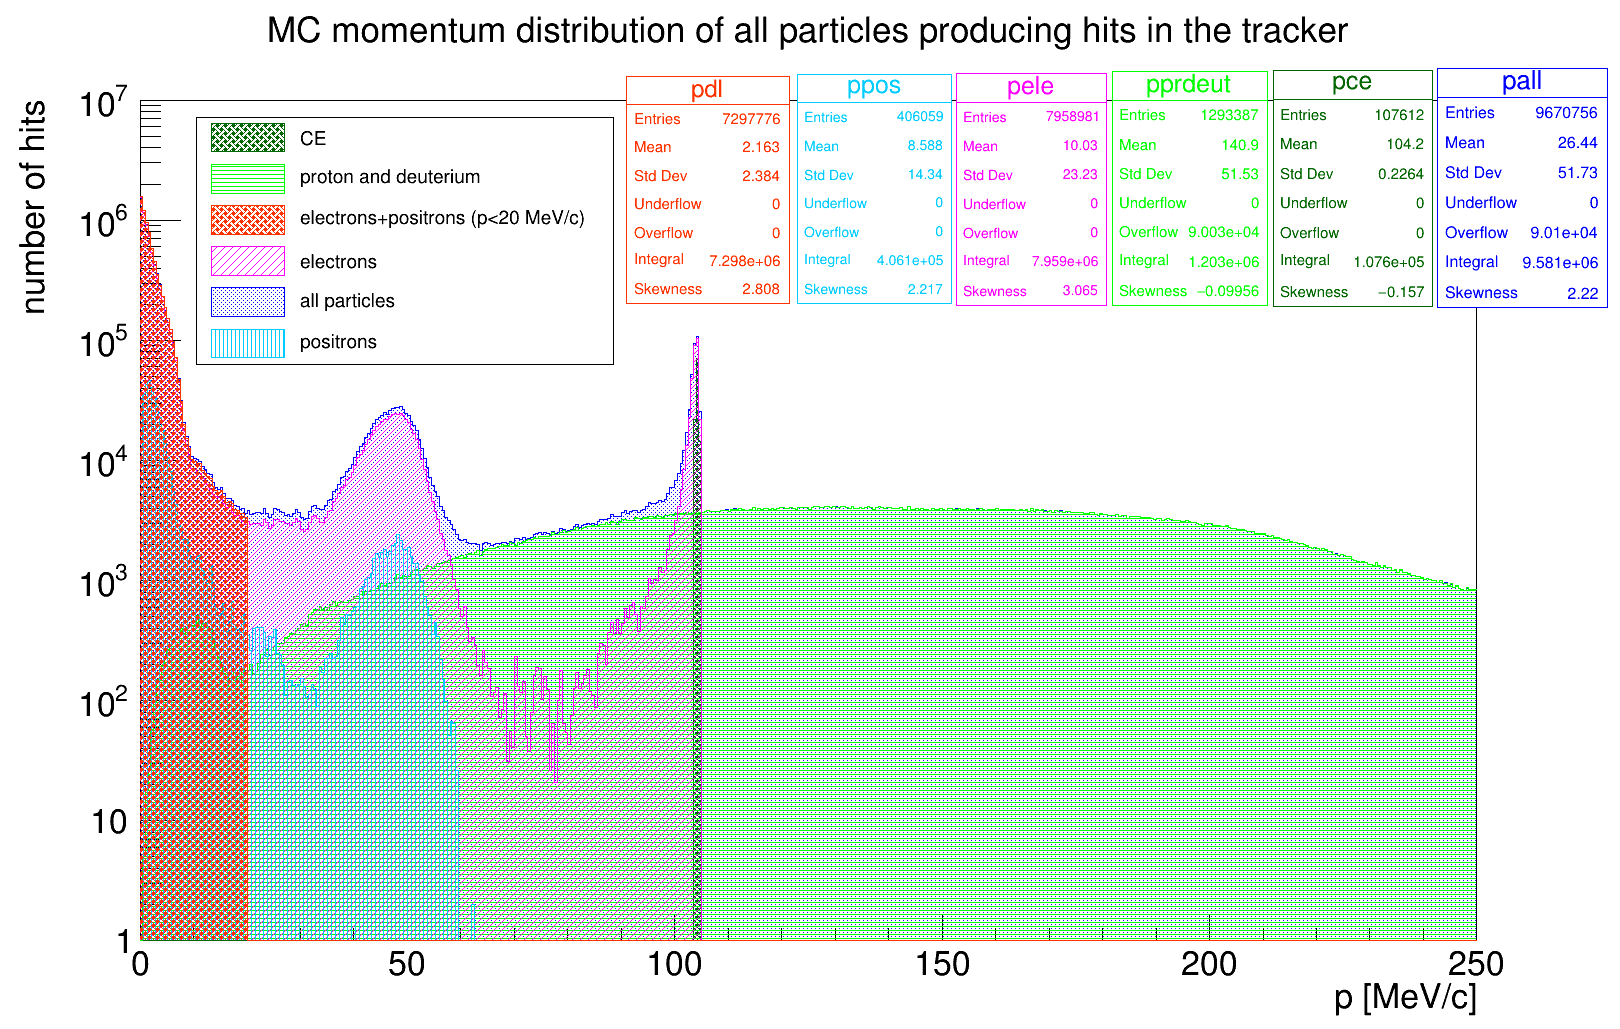
\includegraphics[width =1.1\columnwidth]{figures/png/Screenshot_20240812_152905.png}
       \label{fig:momhits}
\end{figure}
        \end{column}
        \begin{column}{0.5\framewidth}
               \begin{figure}[!h]
        \centering
         \hspace*{-1em}
        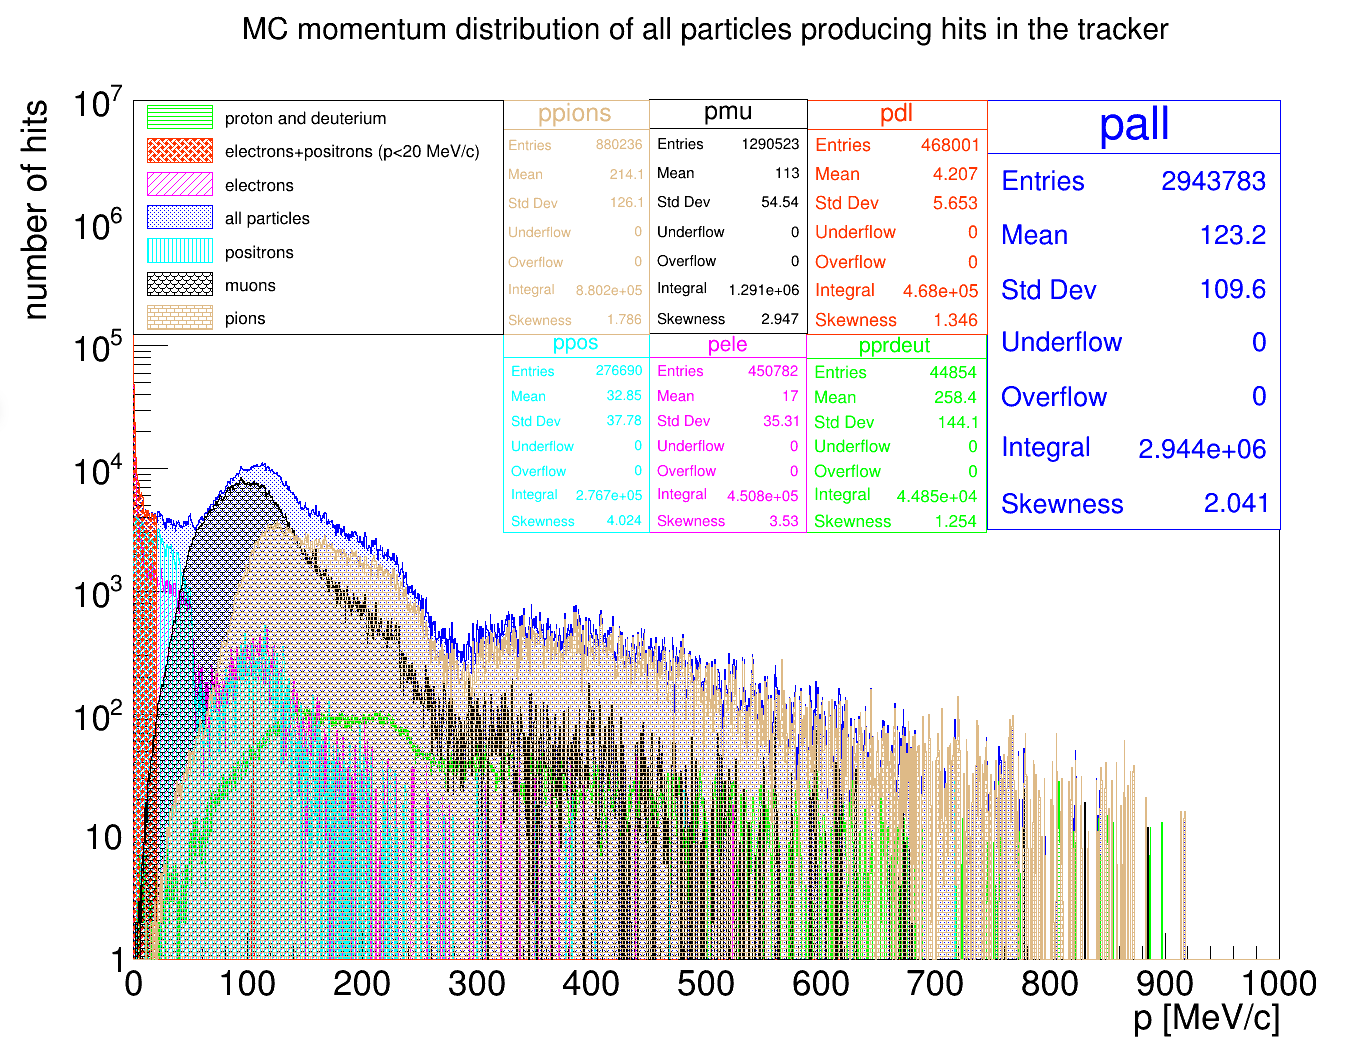
\includegraphics[width =0.95\columnwidth]{figures/png/Screenshot_20240815_124710.png}
       \label{fig:momhits}
\end{figure}
        \end{column}
    \end{columns}
    \vspace{-3mm}
    \begin{columns}
        \begin{column}{1.15\framewidth}
    \setlength{\leftmargini}{1.2em}
    \begin{itemize}
    {\footnotesize
            \item Momentum distribution of particles making at least one hit in the tracker (Left: \textbf{CE-1BB}, Right: \textbf{PBAR-0BB});
            \vspace{2.5mm}
            \item (Left): 75\% of hits by $\delta$-electrons (71\% $e^-$, 4\% $e^+$ - Compton scattering);
              \vspace{2.5mm}
            \item (Left): bump in the $e^+$ distribution ($N(\mu^+ \rightarrow e^+ )/N(\mu^- \rightarrow e^-) \sim 10^{-3}$ for $\mu$ entering the DS and DIO on IPA should be also $10^{-3}$ wrt $\mu^-$ DIF);
              \vspace{2.5mm}
            \item  (Right): $p\bar{p}$ annihilation in ST $\rightarrow$ multiple tracks with $p \sim 100/200$ MeV/c.
          
}
           \end{itemize} 
        \end{column}
      
    \end{columns}
\end{frame}




\begin{frame}
    \frametitle{$\delta$-electrons flagging algorithms}
      \begin{columns}
        \begin{column}{1.15\framewidth}
       {\footnotesize Two \textbf{pre-pattern recognition  algorithms} developed in Mu2e Offline:}
    \setlength{\leftmargini}{1.2em}
    \vspace{0.5mm}
    \begin{itemize}
    {\footnotesize   
    \item \textbf{FlagBkgHits} (FBH). \\ It finds clusters of hits close in $x-y$ and time and ANN to classify them. \\ Based on $StereoHit$ reconstruction. \\ Supervised training with CE+pileup dataset;
    \vspace{0.5mm}
    \item \textbf{DeltaFinder} (DF):
    }
    \begin{itemize}
        {\footnotesize \item $\delta$ segments in each station ($seed$s);
\item  straws' center of gravity on $x$-$y$; 
\item $seed$s across stations connected ($\delta$ candidate); 
\item $p$ candidates ($seed$s with $\bar{E}_{dep}> 3$ keV).}
    \end{itemize}
    \end{itemize}
    \end{column}
    \end{columns}
    \vspace{-3mm}
        \begin{columns}
        \begin{column}{0.5\framewidth}
            \begin{figure}[!h]
        \centering
        \hspace*{-2em}
        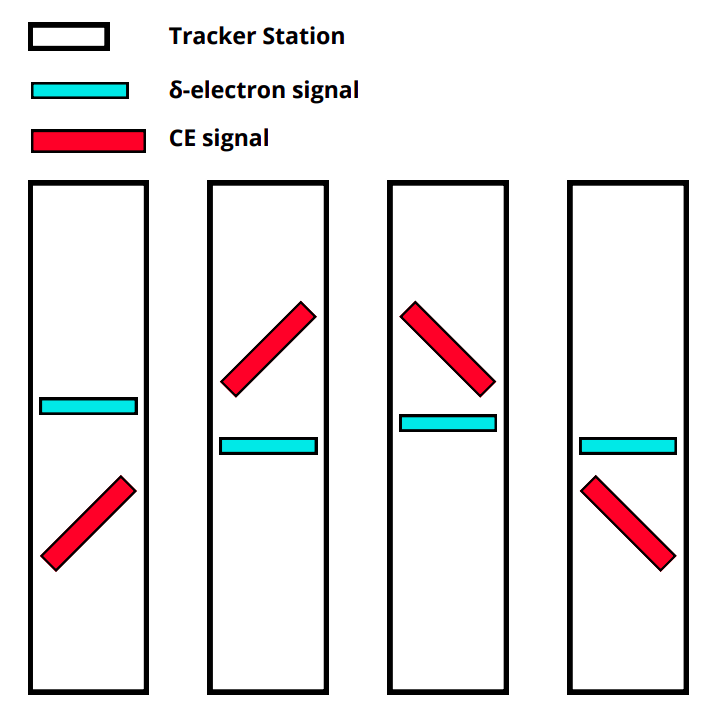
\includegraphics[width =0.6\columnwidth]{figures/png/Screenshot_20240811_123048.png}
       \label{fig:momhits}
\end{figure}
        \end{column}
        \begin{column}{0.5\framewidth}
               \begin{figure}[!h]
        \centering
         \hspace*{-1em}
        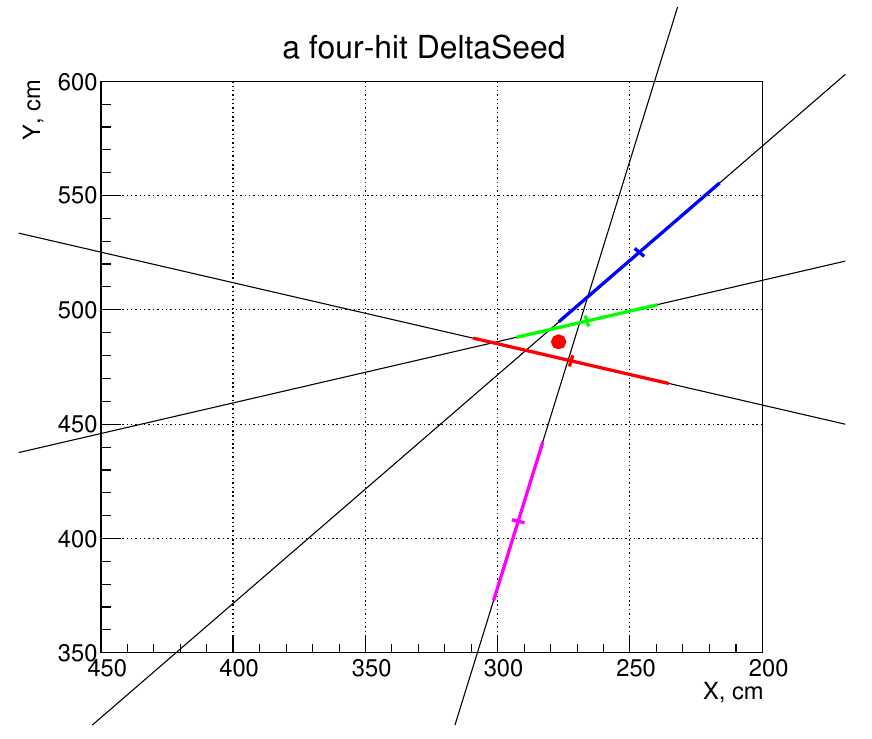
\includegraphics[width =0.75\columnwidth]{figures/png/Screenshot_20240811_115854.png}
       \label{fig:momhits}
\end{figure}
        \end{column}
    \end{columns}
        \vspace{-2mm}
      \begin{columns}
        \begin{column}{1.15\framewidth}
    \setlength{\leftmargini}{1.2em}
    \begin{itemize}
    {\footnotesize   
    \item (Left) $\delta$-electrons and CE in the $r-z$ plane, (Right) $\delta$ candidate $seed$.}
    \end{itemize}
    \end{column}
    \end{columns}
\end{frame}

\begin{frame}
\frametitle{Performance analysis and comparison}
  \begin{columns}
        \begin{column}{1.15\framewidth}
       {\footnotesize Two levels of comparison:}
    \setlength{\leftmargini}{1.2em}
    \begin{itemize}
      {\footnotesize  \item \textbf{hit-level}: how accurately individual hits are flagged (most direct method);
    \item \textbf{high-level}: reconstruction level comparison (figure of merit: CE tracks).
    \vspace{-1mm}
\item Before comparing: \textbf{proton hit flagging over-efficiency} by \textbf{DF}.}
    \end{itemize}
    \end{column}
    \end{columns}
        \vspace{-1mm}
       
        \begin{figure}[!h]
            \centering
            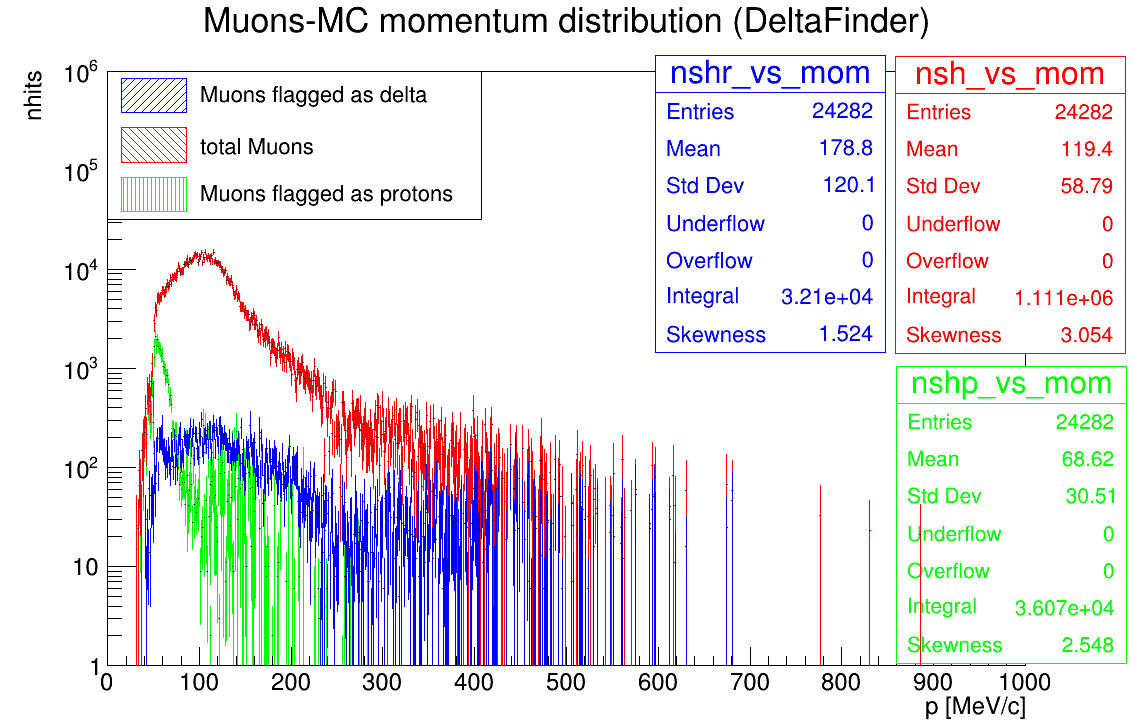
\includegraphics[width =0.5\textwidth]{figures/png/Screenshot_20240805_222923.png}
           \label{fig:0pbarbefore}
        \end{figure}
        
 
    \vspace{-3mm}
    \begin{columns}
        \begin{column}{1.15\framewidth}
    \setlength{\leftmargini}{1.2em}
    \begin{itemize}
      {\footnotesize  
\item (Right): total (red) and flagged (green) $\mu$ hits vs the particle momentum;
\vspace{1mm}
\item Low momentum: higher energy deposition as $p$;
\vspace{1mm}
\item $Good\ proton\ candidate\ \rightarrow\ \geq 4$
hits with $E_{dep} > 3$ keV; 
\item $\epsilon_p$ reduced of 10\%, but $\mu$ and $\pi$ $f_p$ reduced by factor of 2 and 6.
}
      \end{itemize}
      \end{column}
      \end{columns}
\end{frame}




\begin{frame}
    \frametitle{Hit-level comparison}
    \vspace{-3mm}
    \begin{columns}
    \begin{column}{0.45\framewidth}
        \setlength{\leftmargini}{0.7em}
\begin{itemize}
{\footnotesize
    \item $f_p$ and $f_e$: fraction of hits flagged as $p$ and $e^-$;
    \vspace{2mm}
    \item \textbf{No $p$ flagging comparison};
    \vspace{2mm}
    \item (Top Tab): \textbf{PBAR}. $\mu$ and $\pi$ $f_{e,FBH}$ 4x and 3.3x higher;
    \vspace{2mm}
      \item $\pi$: higher momenta;
      \vspace{2mm}
      \item (Bottom Tab): \textbf{CE-1BB}. Same results for \textbf{CE-2BB} within 1\%;
      \vspace{2mm}
      \item \textbf{70\% more CE hits flagged as $\delta$s by FBH wrt DF;}
      \vspace{2mm}
      \item (Bottom): $e^-$ and $e^+$ $f_e$ vs momentum (FBH);
      \vspace{2mm}
      \item 1-2 MeV: Compton;
      \vspace{2mm}
      \item $>2$ MeV: larger $xy$ spread.
    }
\end{itemize}
        \end{column}
         \begin{column}{0.65\framewidth}
        \begin{table}[h!]
        \centering
        \hspace*{-0.5em}
        \renewcommand{\arraystretch}{0.7}
        \begin{tabular}{| c | c | c | c|} 
        \hline
         &  {\scriptsize $f_{p}$ DF} &  {\scriptsize $f_{e}$ FBH} & {\scriptsize $f_{e}$ DF}\\
        \hline
        {\scriptsize $\mu$} &  {\scriptsize 2.7\%}  & {\scriptsize 13.0\%} & {\scriptsize 3.2\%}\\
        \hline
        {\scriptsize $\pi$} & {\scriptsize 0.4\%} & {\scriptsize 23.8\%} & {\scriptsize 7.3\%} \\
        \hline
        \end{tabular}
        \label{tab:0bbpbar}
        
        \end{table}
        \vspace{-6mm}
        \begin{table}[h!]
    \centering
            \hspace*{-0.5em}
    \renewcommand{\arraystretch}{0.7}
    \begin{tabular}{| l | c | c | c |} 
    \hline
    &    {\scriptsize $f_{p}$ DF} & {\scriptsize $f_{e}$ FBH } & {\scriptsize $f_{e}$ DF} \\
    \hline
    {\scriptsize $e^-$} {\tiny[80,110] MeV/c}  & {\scriptsize 0.3\%}  &  {\scriptsize 5.7\%} & {\scriptsize 3.4\%}\\
    \hline
    {\scriptsize $e^-$} {\tiny$<$20 MeV/c}      & {\scriptsize 2.5\%}   & {\scriptsize 75.9\%} & {\scriptsize 72.5\%}\\
    \hline
    {\scriptsize $e^+$} {\tiny$<$20 MeV/c} & {\scriptsize 0.2\%}    &   {\scriptsize 85.5\%}& {\scriptsize 88.5\%}\\
    \hline
  

    \end{tabular}
    
    \end{table}
   
    \begin{figure}[!h]
        \centering
        \hspace*{-2.1em}
        \includegraphics[width =0.8\columnwidth]{figures/png/Screenshot_20240818_155835.png}
       \label{fig:0pbarbefore0}
\end{figure}

 
   
       
\end{column}
\end{columns}

       
   
   
\end{frame}

\begin{frame}
    \frametitle{High-level comparison}
        \vspace{-1mm}
     \begin{columns}
    \begin{column}{0.5\framewidth}
    \vspace{-4mm}
        \setlength{\leftmargini}{0.7em}
\begin{itemize}
{\footnotesize
    \item (Top Tab): \textbf{PBAR}. DF has 22\% advantage in reconstructing 2 tracks (hit-level);
    \item (Bottom Tab): \textbf{CE-1BB}. Same CE reconstruction efficiency (the hit-level difference is 1 hit/track);

    }
\end{itemize}
        \end{column}
         \begin{column}{0.6\framewidth}
        \begin{table}[h!]
        \centering
        \hspace*{-0.5em}
        \renewcommand{\arraystretch}{0.7}
           \begin{tabular}{| c | c | c |} 
            \hline
            {\scriptsize fraction of events} &  {\scriptsize FBH } &  {\scriptsize DF}\\
            \hline
              {\scriptsize $N_{tracks} (\mu, \pi)\geq 2$} &   {\scriptsize 1.8\%} &  {\scriptsize 2.2\%}\\
            \hline
            \end{tabular}
        \label{tab:0bbpbar}
        \end{table}
        \begin{table}[h!]
    \centering
            \vspace{-4mm}
            \hspace*{-0.5em}
    \renewcommand{\arraystretch}{0.7}
    \begin{tabular}{| c | c | c |} 
    \hline
    & {\scriptsize FBH} & {\scriptsize DF}  \\
    \hline
    {\scriptsize CE events with $N_{tracks}>0$} & {\scriptsize 37.9\%} & {\scriptsize 37.9\%} \\
    \hline
    \end{tabular}
    \label{tab:2bbcele}
    \end{table}
        \end{column}
    \end{columns}
    \vspace{-4mm}
 \begin{columns}
        \begin{column}{1.15\framewidth}
    \setlength{\leftmargini}{1.1em}
    \begin{itemize}
    {\footnotesize   
    \item (Bottom): FBH (blue) \& DF (red) reconstructed tracks momentum distributions (two different ranges);
    \item FBH flags less proton hits and these hits are sent to pattern recognition.
    }
    \end{itemize}
    \end{column}
    \end{columns}
        \vspace{-6mm}
     \begin{columns}
        \begin{column}{0.5\framewidth}
            \begin{figure}[!h]
        \centering
        \includegraphics[width =0.9\columnwidth]{figures/png/Screenshot_20240820_162125.png}
       \label{fig:momhits}
\end{figure}
        \end{column}
        \begin{column}{0.5\framewidth}
               \begin{figure}[!h]
        \centering
        \includegraphics[width =0.9\columnwidth]{figures/png/Screenshot_20240820_160904.png}
       \label{fig:momhits2}
\end{figure}
        \end{column}
    \end{columns}
\end{frame}







\begin{frame}
    \frametitle{Outline}
\begin{itemize}
	\item \textcolor{mygray}{Commissioning of the tracker DAQ and FEE:}
	\begin{itemize}
        \vspace{2mm}
    	\item \textcolor{mygray}{validation of ROC readout;}
        \vspace{1.5mm}
    	\item \textcolor{mygray}{study of preamplifiers performance}.
	\end{itemize}
	\vspace{4mm}
    	\item \textcolor{mygray}{First steps towards the station calibration;}
    	\vspace{6mm}
    	\item \textcolor{mygray}{Pre-pattern recognition studies;}
  	\vspace{6mm}
    	\item Conclusions.
\end{itemize}
\end{frame}

\begin{frame}{Conclusions}
\vspace{-3mm}
\begin{columns}
\begin{column}{1.15\framewidth}
 \setlength{\leftmargini}{1.2em}
    \begin{itemize}
        {\footnotesize
\item \textbf{CLFV} processes provide a clean test field for \textbf{NP models};
\vspace{1.2mm}
\item \textbf{Mu2e} is one of the leading experiments and searches for $ \mu^- N \rightarrow e^- N $;
\vspace{1.2mm}
\item Tracker performance is crucial;
\vspace{1.2mm}
    \item \textbf{Comprehensive study} from the tracker readout to offline analysis:}
   \begin{itemize}
      \vspace{1.2mm}
      {\footnotesize \item \textbf{DAQ} and \textbf{FEE} testing:}
   \vspace{1mm}
      \begin{itemize}
          
     
        {\footnotesize  \item \textbf{ROC readout validation} with MC at a level of $10^{-3}$;
        \vspace{1mm}
    \item \textbf{Preamps}: dead channels, 
cross-talk, and waveform patterns study.}
 \end{itemize}
    \vspace{1.2mm}
    {\footnotesize \item \textbf{First steps towards timing calibration}:}
  \vspace{1mm}
 \begin{itemize}
    {\footnotesize  \item \textbf{Vertical station orientation} $\rightarrow$ non-uniform panel illumination;
    \vspace{1mm}
     \item Large \textbf{bias} on $x_{track}$ reconstruction ($\pm$4 cm) $\rightarrow$ data-taking time.
    }
 \end{itemize}
   \vspace{1.2mm}
   {\footnotesize \item \textbf{Pre-pattern recognition study} to flag $\delta$-electrons:}
  \vspace{1mm}
  \begin{itemize}
    {\footnotesize  \item \textbf{Hit-level}: FBH flags 70\% more CE hits, same performance for $\delta$s, no possible $p$ flag comparison, FBH not trained on $\bar{p}$ data sample;
    \vspace{1mm}
    \item \textbf{High-level}: same recostruction performance for CE signal;
  \vspace{1mm}
  \item  \textbf{Timing}: 0.13, 0.39 ms/ev (1BB, 2BB) more for DF vs 5 ms/ev expected.}
 \end{itemize}
   \end{itemize}
    \end{itemize}
    \end{column}
\end{columns}

\end{frame}



\begin{frame} % and our simple frame
    \begin{center}
            \LARGE{\textbf{Thank you for your attention!}}
    \end{center}
\end{frame}
\begin{frame}{Bibliography} % and our simple frame
\begin{columns}
    \begin{column}{1.04\framewidth}
            \setlength{\leftmargini}{1.05em}
    \bibliographystyle{siam}
   {\footnotesize \bibliography{presentazione.bib}}
    \end{column}
\end{columns}

\end{frame}
\begin{frame} % and our simple frame
    \begin{center}
            \LARGE{\textbf{BACKUP SLIDES}}
    \end{center}
\end{frame}

\begin{frame}
    \frametitle{Beyond the SM}
    \vspace{-3mm}
  
        \begin{columns}
            \begin{column}{1.15\framewidth}
            \setlength{\leftmargini}{1.1em}
        \begin{itemize}
    {\footnotesize   \item  \textbf{Supersymmetry}:} 
    \begin{itemize}
        {\footnotesize \item particle with superpartner (different spin), lepton $\rightarrow \ slepton$;
        \item no common mass eigenstate base $\rightarrow$ 
        $slepton$ superposition of flavours;
        \item CLFV suppression mitigated by $\nu$ and $W$ superpartners;
        \item SUSY breaking at electroweak scale ($\sim 10^2$ GeV) $\rightarrow$ observable 
        violation. 
        }
    \end{itemize}
    {\footnotesize  \item \textbf{Two Higgs Doublet model}:}
    \begin{itemize}
        {\footnotesize  \item  two Higgs bosons each interacting with fermions;
        \item non-zero-off-diagonal terms $\rightarrow$ flavour violating Yukawa couplings.}
    \end{itemize}
    {\footnotesize  \item \textbf{Leptoquark models}:}
    \begin{itemize}
        {\footnotesize   \item LQ has both a baryon and lepton number; 
        \item quark and lepton sectors are unified $\rightarrow$ direct coupling via LQ exchange;
        \item specific CLFV processes are mediated by LQs.}

    \end{itemize}
    {\footnotesize  \item  \textbf{Additional Neutral Gauge Boson}: }
    \begin{itemize}
        {\footnotesize   
        \item lower energies: gauge groups break down to the 
        direct product of the SM Gauge group $SU(3) \times SU(2) \times U(1)$ 
        along with an additional $U(1)$ factor;
        \item neutral gauge boson mixes with SM neutral Gauge boson;
        \item two mass eigenstates ($Z$, $Z'$);
        \item off-diagonal terms in neutral current couplings 
        to fermions can lead to flavour-changing couplings to $Z$ and $Z'$.}

    \end{itemize}


\end{itemize}
\end{column}
\end{columns}
\end{frame}


\begin{frame}
    \begin{figure}[h]
        \centering
        \includegraphics[width=1.\textwidth]{figures/png/Screenshot_20240927_131322.png}
    \end{figure} 
    \begin{columns}
        \begin{column}{0.5\framewidth}
    \begin{figure}[!h]
        \centering
        \includegraphics[width =0.55\columnwidth]{figures/png/Screenshot_20240218_105920.png}
        \label{fig:susy}
        \end{figure}
    \end{column}
    \begin{column}{0.5\framewidth}
   {\small SUSY contribution to $l_i \rightarrow l_j\gamma$ via $slepton$ }
    \end{column}
\end{columns}
\end{frame}







\begin{frame}
    \frametitle{Muon channels}
    \vspace{-3mm}
    \begin{columns}
     \begin{column}{1.15\framewidth}
     \setlength{\leftmargini}{1.1em}
    
        \begin{itemize}
       {\small   
       \item $\mu$ production favored in $\pi$ and $K$ decays by hadronic interactions;
       \vspace{0.9mm}
       \item Long lifetime $\rightarrow$ muon beams;
       \vspace{0.9mm}
       \item Small mass: limited number of decay modes available;
       \vspace{0.9mm}
       \item $\mu^+ \rightarrow e^+ \gamma$:
        \vspace{0.7mm}
       }
       \begin{itemize}
        {\small \item $e^-$ and $\gamma$ (52.8 MeV back-to-back);
         \vspace{0.7mm}
        \item $ \mu^+ \ \rightarrow$ no nuclear capture;
         \vspace{0.7mm}
        \item Radiative Muon Decay $\mu^+ \rightarrow e^+ \nu_e \bar{\nu}_\mu \gamma$;
         \vspace{0.7mm}
        \item Accidental Coincidence of $\mu^+ \rightarrow e^+ \nu_e \bar{\nu}_\mu$ with a $\gamma$; 
         \vspace{0.7mm}
        \item Continuous beam.
        }
       \end{itemize}
       \vspace{0.9mm}
       \item $\mu^+ \rightarrow e^+ e^- e^+$:
        \vspace{0.7mm}
       \begin{itemize}
        {\small \item 2 $e^+$ and 1 $e^-$ with total energy equal to the $M_\mu$;
         \vspace{0.7mm}
        \item Momentum range from few MeV to $M_\mu/2 \ \rightarrow$ tracker resolution;
         \vspace{0.7mm}
        \item Radiative Muon Decay $\mu^+ \rightarrow e^+ \nu_e \bar{\nu}_\mu \gamma$ with internal conversion;
         \vspace{0.7mm}
        \item Coincidence of one Michel decay with $e^+e^-$ pair (1-MD) or 
        two Michel decays with $e^+$ (2-MD);
         \vspace{0.7mm}
        \item Continuous beam.

        }
       \end{itemize}
        \end{itemize}
    \end{column}
\end{columns}
\end{frame}
\begin{frame}{Muon channels}
    \vspace{-1mm}
    \setlength{\leftmargini}{0em}
    \begin{itemize}
    \item \textbf{EFT} Lagrangian parametrisation (model-indipendent): $\Lambda$ is the effective mass scale and $\kappa$ controls the relative contribution of the dipole moment term and the contact term.
    \end{itemize}
    \begin{equation*}\label{LCF}
    \mathcal{L}_{C L F V}=  \frac{m_\mu}{(1+\kappa) \Lambda^2} \bar{\mu}_R \sigma_{\mu \nu} e_L F^{\mu \nu}+ \frac{\kappa}{(1+\kappa) \Lambda^2} \bar{\mu}_L \gamma_\mu e_L\left(\sum_{q=u, d} \bar{q}_L \gamma^\mu \bar{q}_L\right)
    \end{equation*}
    \vspace{-3mm}
    \begin{columns}
    \begin{column}{0.5\framewidth}
                    \begin{figure}[h]
                \centering
                \hspace*{-6ex}
                \includegraphics[width=0.8\columnwidth]{figures/png/Screenshot_20240913_151711.png}
            \end{figure} 
            \begin{figure}[h]
                \centering
                \hspace*{-6ex}
                \includegraphics[width=0.8\columnwidth]{figures/png/Screenshot_20240913_151719.png}
            \end{figure}  
        \end{column}
        \begin{column}{0.5\framewidth}
            \begin{figure}[h]
                \centering
                \hspace*{-6ex}
                \includegraphics[width=0.85\columnwidth]{figures/png/Screenshot_20240313_120457.png}
            \end{figure}  
        \end{column}
    \end{columns}
    
    \end{frame}



    \begin{frame}
        \frametitle{$\mu^+ \rightarrow e^+ \gamma$ experiments}
        \vspace{-3mm}
\begin{columns}
 \begin{column}{0.66\framewidth}
 \setlength{\leftmargini}{1.1em}
    \begin{itemize}
   {\small     \item  \textbf{MEG}:}
         \begin{itemize}
             {\small 
             \item polyethylene target to stop $\mu$s;
             \vspace{0.5mm}
            \item anti-bottle $B$ decreases uniformly from centre, pushing particles away; 
            \vspace{0.5mm}
            \item low energy $e^+$ discarded $\rightarrow$ detector far from magnet axis;
            \vspace{0.5mm}
            \item drift chamber and timing counters to measure the $p_{e^+}$ and timing;
            \vspace{0.5mm}
            \item LXe detector for $E_e$ and $E_\gamma$.
            }
   \end{itemize}
   {\small      \item  \textbf{MEG II}:}
               \begin{itemize}
                {\small \item to reduce the accidental background;
                \vspace{0.5mm}
                \item muon flux increased ({\footnotesize$7 \times 10^7 \ \mu^+$/s});
                \vspace{0.5mm}
                \item thinner but more inclined ST;
                \vspace{0.5mm}
                \item new cylindrical drift chamber (higher granularity and transparency);
                \vspace{0.5mm}
                \item pixellated-TC;
                \vspace{0.5mm}
                \item Radiative Decay Counter (low angle $e^+$).
                }
                \end{itemize}
    \end{itemize}
    \end{column}
    \begin{column}{0.5\framewidth}
        \begin{figure}[!h]
            \centering
            \includegraphics[width =\columnwidth]{figures/png/Screenshot_20240321_115127.png}
            \end{figure}
            \begin{figure}[!h]
                \centering
                \includegraphics[width =\columnwidth]{figures/png/Screenshot_20240307_140116.png}
                \end{figure}
    \end{column}

\end{columns}
    \end{frame}
  

    \begin{frame}
        \frametitle{$\mu^+  \rightarrow e^+ e^- e^+$ experiments}
        \vspace{-3mm}
\begin{columns}
 \begin{column}{0.65\framewidth}
 \setlength{\leftmargini}{1.1em}

    \begin{itemize}
        {\small     \item \textbf{SINDRUM I}:  }
        \begin{itemize}
            {\small \item  double cone stopping target in the 
            middle of five concentric multi-wire proportional chambers 
            surrounded by plastic scintillator counters;
            \vspace{1mm}
            \item solenoidal magnetic field;
            \vspace{1mm}
            \item momentum resolution at the level of $\sim$1 MeV, 
            timing resolution $\leq$1 ns and a vertex resolution of $\sim$1 cm.
            }
        \end{itemize}
   {\small     \item \textbf{Mu3e}: 
   }
   \begin{itemize}
    {\small \item  goal of SES$\sim 10^{-16}$;
    \vspace{1mm}
    \item muons stopped on a thin hollow double-cone Mylar target;
    \vspace{1mm}
    \item 2 m cylinder detector placed inside a 1.5 T magnetic field in 5 sections;
    \vspace{1mm}
    \item pixel detectors and scintillating fiber.
    }
\end{itemize}


    \end{itemize}
    \end{column}
    \begin{column}{0.5\framewidth}
        \begin{figure}[!h]
            \centering
            \includegraphics[width =\columnwidth]{figures/png/The-SINDRUM-I-detector-in-the-horizontal-operating-orientation.png}
            \label{fig:sindrumi}
            \end{figure}
            \begin{figure}[!h]
                \centering
                \includegraphics[width =\columnwidth]{figures/png/Screenshot_20240321_143650}
                \label{fig:mu3e}
                \end{figure}
    \end{column}
\end{columns}
    \end{frame}



















    \begin{frame}
        \frametitle{$ \mu^- N \rightarrow e^- N $ experiments}
        \vspace{-3mm}
\begin{columns}
 \begin{column}{0.67\framewidth}
 \setlength{\leftmargini}{1.1em}

    \begin{itemize}

        {\small    
   
   \item \textbf{SINDRUM II}: }

\begin{itemize}
    {\small  
    \item cylindrical structure;
    \item target in the middle of the detector;
    \item 2 drift chambers (CO$_2$-C$_4$H$_10$ and He-C$_4$H$_10$); 
    \item plastic scintillators and Cherenkov for timing and triggering;
    \item stopped $\mu$: Ge(Li) detector.
    }
\end{itemize}


   {\small    
   
   \item \textbf{COMET}: }
  \begin{itemize}
    {\small  
    \item  C-shaped transport solenoid: tighter
    muon momentum selection, with a reduced beam intensity ($\sim$30\% less);
    \item additional curved solenoid after 
    the stopping target (to remove $e^-$);
    \item Phase-I: understand experimental 
    techniques and backgrounds;
    \item Phase-II: straw tube 
    tracker and a LYSO EM  
    calorimeter. Magnetic system expanded.
    }
  \end{itemize}
    \end{itemize}
    \end{column}
    \begin{column}{0.5\framewidth}
        \begin{figure}[!h]
            \centering
            \includegraphics[width =0.9\columnwidth]{figures/png/Screenshot_20240307_163120.png}
            \label{fig:sindrumii}
            \end{figure}
            \begin{figure}[!h]
                \centering
                \includegraphics[width =0.9\columnwidth]{figures/png/Screenshot_20240307_152133.png}
                \label{fig:comet}
                \end{figure}
    \end{column}
\end{columns}
    \end{frame}


   









\begin{frame}
    \frametitle{Tau channel}
    \vspace{-3mm}
    \begin{columns}
     \begin{column}{1.15\framewidth}
     \setlength{\leftmargini}{1.1em}
    
        \begin{itemize}
       {\small     \item  $\tau$: promising source of CLFV decays;
       \vspace{1mm}
       \item Large mass ($m_\tau$ $\sim$ 1.777 GeV) $\rightarrow$ multiple CLFV channels;
       \vspace{1mm}

       \item $\tau \rightarrow l \gamma$ (radiative decay), $\tau \rightarrow 3l$ (three-body decay) 
       and $\tau\rightarrow l \ h$;
       \vspace{1mm}

            \item No beams $\rightarrow \ \tau_\tau \ \sim$ 2.9 $\times$ 10$^{-13}$ s;
            \vspace{1mm}

\item    Large detectors with good PID, tracking, calorimetry, hermeticity required; 
\vspace{1mm}

\item $\tau^+ \tau^-$ produced by $\Upsilon(4s)$ resonance at $\sqrt{s}=10.58$ GeV;
\vspace{1mm}

        \item Wide-range calibrations for detectors.  
       }
    \end{itemize}
\end{column}
\end{columns}
   
    \begin{figure}[!h]
      \centering
      \includegraphics[width =0.6\textwidth]{figures/png/Screenshot_20240319_134052.png}
      \label{fig:tauchannel}
      \end{figure}
  
\end{frame}


   


\begin{frame}
    \begin{center}  
        \begin{table}[!h]
        \centering
        \renewcommand{\arraystretch}{1}
        \begin{tabular}{c c c c c}
        \hline
        Reaction & Present limit & CL & Experiment &  Year \\
        \hline
        $\mu^+\ \rightarrow \ e^+ \ \gamma$& $7.5 \times 10^{-13}$ & 90\% & MEG II & 2024 \\
        $\mu^+ \ \rightarrow \ e^+ \ e^+ \ e^-$ & $1.0 \times 10^{-12}$ & 90\% & SINDRUM & 1988 \\
        $\mu^- \ \text{Ti}\ \rightarrow \ e^- \ \text{Ti}$ &  $6.1 \times 10^{-13}$ & 90\% & SINDRUM II & 1998\\
        $\mu^- \ \text{Au}\ \rightarrow \ e^- \ \text{Au}$ & $7.0 \times 10^{-13}$ & 90\% & SINDRUM II & 2006  \\
        $\mu^+ \ e^- \ \rightarrow \ \mu^- \ e^+$ & $8.3 \times 10^{-11}$ & 90\% & SINDRUM & 1999 \\
        $\tau \ \rightarrow \ e \ \gamma$ & $3.3 \times 10^{-8}$ & 90\% & BaBar & 2010 \\
        $\tau \ \rightarrow \ \mu \ \gamma$ & $4.4 \times 10^{-8}$ & 90\% & BaBar & 2010 \\
        $\tau \ \rightarrow \ e \ e \  e$ & $2.7 \times 10^{-8}$ & 90\% & Belle & 2010 \\
        $\tau \ \rightarrow \ \mu \ \mu  \ \mu$ & $2.1 \times 10^{-8}$ & 90\% & Belle & 2010  \\
        \hline
        \end{tabular}
        \caption{Experimental upper limits for CLFV processes (leptons).}
        \label{tab:upperlimits}
        \end{table}
    \end{center}
    \end{frame}








    \begin{frame}
        \frametitle{Pulsed proton beam}
        \vspace{-3mm}
    \begin{figure}[!h]
    \centering
    \includegraphics[width =0.9\textwidth]{figures/png/Screenshot_20240301_164649.png}
    \label{fig:beamwindow}
    \end{figure}
    \begin{columns}
        \begin{column}{1.15\framewidth}
        \setlength{\leftmargini}{1.1em}
       
           \begin{itemize}
          {\small     \item 8 GeV, 8 kW beam originates from the Fermilab Booster;
          \item Proton pulses separated by 1695 ns and the delayed window is after 640 ns after the first pulse;
          \item Due to the short lifetime of pions, this background can be suppressed by using pulsed
          proton beam along with a delayed live-time window.
          }
           \end{itemize}
       \end{column}
       \end{columns}
    \end{frame}




\begin{frame}
    \frametitle{Mu2e beamline}
    \begin{figure}[!h]
        \centering
        \includegraphics[width =0.7\textwidth]{figures/png/Screenshot_20240303_152845.png}
        \label{fig:muonbeamline}
        \end{figure}
        \begin{figure}[!h]
            \centering
            \includegraphics[width =0.6\textwidth]{figures/png/800px-MuonBeamlineCollimators2.png}
            \label{fig:collimators}
            \end{figure}
    \end{frame}

\begin{frame}
    \frametitle{Why Al Stopping Target?}
    \vspace{-3mm}
\begin{columns}
 \begin{column}{0.65\framewidth}
 \setlength{\leftmargini}{1.1em}
 \vspace{-3mm}
    \begin{itemize}
   {\small     \item Lower RMC background. Photon endpoint: {\footnotesize $k_{max} = m_\mu c^2 - |E_b| - E_{rec} - \Delta M$ }
        \\
        $\sim$101.9 MeV; 
        \vspace{3mm}
\item Long lifetime: better separation between prompt backgrounds and live window; 

\vspace{3mm}
\item High Al DIO endpoint: Higher-$Z$ nuclei $\rightarrow$ lower endpoint, minimizing background contribution;
\vspace{3mm}
\item Conversion $BR$ depends on the ST material. Materials with higher $Z$ $\rightarrow$ better model differentiation (Mu2e-II: Ti);
\vspace{3mm}
\item Available in required size/shape/thickness, low costs and chemically stable.}
    \end{itemize}
\end{column}   
 \begin{column}{0.5\framewidth}
    \begin{figure}[!h]
        \centering
        \includegraphics[width=0.8\columnwidth]{figures/png/lifetime_mu_matter.png}
        \label{fig:muonicatom}
 \end{figure}
       \begin{figure}[!h]
        \centering
        \includegraphics[width=0.8\columnwidth]{figures/png/endopint.png}
        \label{fig:endpoint}
    \label{fig:2imins}
  \end{figure}
\end{column}   
\end{columns}

\end{frame}

\begin{frame}
    \frametitle{The electromagnetic calorimeter}
    \begin{columns}
            \begin{column}{0.65\framewidth}
      Calorimeter is vital for:
      \begin{itemize}
          \item \textbf{PID} ($E/p$);
          \item Seed for \textbf{track reconstruction};
          \item Fast online \textbf{trigger} filter.
      \end{itemize}
      \textbf{Design}:
      \begin{itemize}
        \item 2 hollow disks of crystals, 70 cm apart;
          \item 2 $\times$ 674 CsI crystals per disk, each coupled to 2 SiPMs.
      \end{itemize}
      \textbf{Performance}:
      \begin{itemize}
          \item $\sigma_E/E \sim$ 10\%;
          \item $\sigma_{xy}\sim$ 6 mm;
          \item $\sigma_t < 500$ ps.
      \end{itemize}
               \end{column}
        \begin{column}{0.5\framewidth}
            \begin{figure}[h]
            \centering
            \includegraphics[width=\columnwidth]{figures/png/Screenshot_20240322_121000.png}
        \end{figure}
              \begin{figure}[h]
            \centering
            \includegraphics[width=\columnwidth]{figures/png/Screenshot_20240706_151533.png}
        \end{figure}
        \end{column}
    \end{columns}
\end{frame}

\begin{frame}
    \frametitle{Extinction monitor}
    \vspace{-3mm}
    \begin{columns}
        \begin{column}{0.65\framewidth}
            \setlength{\leftmargini}{1.1em}
           
               \begin{itemize}
              {\small  
\item Mu2e requirement: extinction $<10^{-10}$;
\vspace{2mm}
\item Two factors contribute to extinction: }
\vspace{1mm}
\begin{itemize}
    {\small 
\item intrinsic accelerator
extinction ($2.1 \times 10^{-5}$);
\vspace{1mm}
\item Mu2e AC dipoles sweep away out-of-time protons into
collimators ($5\times 10^{-8}$).}
\vspace{2mm}
\end{itemize}
{\small 
\item Extinction Monitor (EM): collimator and magnetic filter 
system, pixel telescope; 
\vspace{2mm}
\item EM measures out-of-time protons;
\vspace{2mm}
\item Magnetic filter transport of particles generated at the PT to the EM;
\vspace{2mm}
\item The pixel telescope tracks the trajectory and momentum of particles (permanent magnet + 8 scintillators).}

              
               \end{itemize}
            \end{column}
            \begin{column}{0.5\framewidth}
                \begin{figure}[!h]
                    \centering
                    \includegraphics[width =\columnwidth]{figures/png/800px-Extinction_filter.png}
                    \label{fig:extintion}
                    \end{figure}
                    \begin{figure}[!h]
                    \centering
                    \includegraphics[width =\columnwidth]{figures/png/Screenshot_20240306_184720.png}
                    \label{fig:extintionmonitor}
                    \end{figure}
            \end{column}
    \end{columns}
\end{frame}


\begin{frame}
    \frametitle{Cosmic Ray Veto and Stopping Target Monitor}
    \vspace{-2mm}
 \begin{columns}
            \begin{column}{0.55\framewidth}
                     \textbf{Cosmic Ray Veto}:
         \begin{itemize}
        {\small \item \textbf{Active veto}: 4 layers of extruded plastic scintillation counters;
                \item \textbf{Passive shielding}: Al absorbers between each layer;
                \item $\epsilon_{CRV}=99.9\%$;
               \item $\mu$'s signature: 3/4 vetoed.}
            \end{itemize}
             \begin{figure}[h]
            \centering
            \includegraphics[width=0.9\columnwidth]{figures/png/Screenshot_20240706_094517.png}
        \end{figure}
            \end{column}
            \begin{column}{0.55\framewidth}
            \begin{figure}[h]
            \centering
            \includegraphics[width=0.8\columnwidth]{figures/jpg/Crv_downstream.jpg}
        \end{figure}
        \textbf{Stopping Target Monitor}:
            \begin{itemize}
                {\small  \item HPGe and  $ \text{LaBr}_3$ detector $\rightarrow$ number of $\mu$ stopped in ST (10\% precision on $N_\mu$);
                \item It will measure the photons produced by secondary muonic aluminium orbital transitions (347 keV) and nuclear capture (884 keV, 1809 keV);
                \item Captured $\mu$ = 61\% of stopped $\mu$.
                }
            \end{itemize}
                         
            \end{column}
    \end{columns}
\end{frame}

\begin{frame}
    \frametitle{Drift tubes}
    \vspace{-4mm}
    \begin{columns}
        \begin{column}{0.65\framewidth}
            \setlength{\leftmargini}{1.1em}
            \begin{itemize}
               {\small 
		\item Cathode: grounded cylindrical conductor;
               \vspace{1.2mm}
               \item Anode wire $\rightarrow$ high voltage $\mathcal{O}(\text{kV})$; 
                \vspace{1.2mm}
                \item Gases combination: noble ($A$) + quench gas ($B$);
                \vspace{1.2mm}
                \item $E(r)=\frac{1}{r}\frac{\lambda}{2\pi \epsilon}=\frac{1}{r}\frac{V}{ \text{ln}(b/a)} \quad (a<r<b)$;
                \vspace{1.2mm}
                \item Primary ionisation: $A \ C \rightarrow A^+ e^- C$, or $A \ C \rightarrow A^{++} e^- e^- C$;
                \vspace{1.2mm}
                \item Excitation: $A \ C \rightarrow A^* C \rightarrow$ $A^* \ B \rightarrow A B^+ e^-$ or $A^* \ A \rightarrow A_2^+ e^-$;
                \vspace{1.2mm}
                \item Secondary ionisation $\rightarrow$ avalanche;
                \vspace{1.2mm}
                \item Proportional region;
                \vspace{1.2mm}
                \item Quench gas (CO$_2$) absorbs $\gamma$s from recombination preventing subsequent 
                avalanches.
                }
            \end{itemize}
        \end{column}
        \begin{column}{0.5\framewidth}
            \begin{figure}[!h]
                \centering
                \includegraphics[width =0.9\columnwidth]{figures/png/Screenshot_20240324_232621.png}
                \label{fig:drifttube}
                \end{figure}
                \begin{figure}[!h]
                    \centering
                    \includegraphics[width =0.9\columnwidth]{figures/png/Screenshot_20240330_182509.png}
                  \label{fig:avalanche}
                  \begin{figure}[!h]
                    \centering
                    \includegraphics[width =0.75\columnwidth]{figures/png/Screenshot_20240330_203416.png}
                    \label{fig:gaseous}
                    \end{figure}
                \end{figure}
        \end{column}
    \end{columns}
\end{frame}



\begin{frame}
    \frametitle{Drift tubes in magnetic field}

    \vspace{-3mm}
    \begin{columns}
        \begin{column}{0.65\framewidth}
            \setlength{\leftmargini}{1.1em}
            
            \begin{itemize}
            
              {\footnotesize \item Electric drift and magnetic field: }
               \begin{itemize}
                {\footnotesize       
                \item drift direction and velocity change ($ B \uparrow \rightarrow v_d \downarrow $); 
                \item reduction of diffusion transverse to the magnetic field.  ciao
                } 
            \end{itemize}

            
               {\footnotesize
               \vspace{1mm}
		\item Type of drift gas and magnetic-electric field relative orientation;
                \vspace{1mm}
                \item $\vec{v}_D^B=-\frac{\mu^{B=0}}{1+\omega^2 \tau^2}\left(\vec{E}+\frac{\vec{E} \times \vec{B}}{B} \omega \tau+\frac{(\vec{E} \vec{B}) \vec{B}}{B^2} \omega^2 \tau^2\right)$;
               \vspace{1mm}
               \item $\mu_B = 0$: mobility with $B=0$;
               \vspace{1mm}
                \item $\omega = \frac{qB}{m}$: cyclotron frequency; 
                \vspace{1mm}
               \item $\tau$: average collision time in the gas;
                \vspace{1mm}
                \item Straws $\perp$ to $B$;
                \vspace{1mm}
                \item $\alpha_{v_d B} \in $(0°,90°);
                \vspace{1mm}
                \item Ar:CO$_2$: $v_{d}$ depends on the electric field;
               \vspace{1mm}
                \item 8 ns at a radial distance of 2.5 mm.}
              
          \end{itemize}
        \end{column}
        \begin{column}{0.5\framewidth}
            \begin{figure}[!h]
                \centering
                \includegraphics[width =0.9\columnwidth]{figures/png/Screenshot_20240925_214957.png}
                \label{fig:driftchange}
                \end{figure}

            \begin{figure}[!h]
                \centering
                \includegraphics[width =0.7\columnwidth]{figures/png/Screenshot_20240330_102206.png}
                \label{fig:drift}
                \end{figure}
        \end{column}
    \end{columns}

    

\end{frame}





\begin{frame}
    \frametitle{Tracker data format}
    \begin{columns}
        \begin{column}{1.15\framewidth}
    \setlength{\leftmargini}{1.em}

    A \textbf{hit data packet} has
    a fixed length of 32 bytes:
    \vspace{2mm}
    \begin{itemize}
        \item 16 bit header (straw index);
        \vspace{1mm}
        \item 16 bit for the TDC left straw end;
        \vspace{1mm}
        \item 16 bit for the TDC right straw end;
        \vspace{1mm}
        \item 8 bits for the ToT (time-over-threshold) for the two ends;
        \vspace{1mm}
        \item 12 bits for each ADC samples. For each hit, a fixed number of 
        samples (15) is readout;
        \vspace{1mm}
        \item 12 bits are set aside for preprocessing flags.
    \end{itemize}
\end{column}
\end{columns}
    \end{frame}



\begin{frame}
    \frametitle{DAQ system}

  
   
       
        \begin{figure}[!h]
            \centering
         
            \includegraphics[width =0.4\textwidth]{figures/png/Screenshot_20240206_144803.png}
            \label{fig:linktodaq}
            \end{figure}
   
\vspace{-1.5mm}
\begin{columns}
    \begin{column}{1.15 \framewidth}
        \setlength{\leftmargini}{1.1em}
        \begin{itemize}
          {\footnotesize 
          \item $Streaming$ readout: digitized and zero-suppressed data, flexible for analysis; 
          \vspace{-0.5mm}
          \item DAQ run control via RCH, managing a 
          predefined Run Plan; 
          \vspace{-0.5mm}
          \item Active spill defined by proton pulses, defining the EW; 
          \vspace{-0.5mm}
          \item CFO module generates 40 MHz clock, embedding EWMs; 
          \vspace{-0.5mm}
          \item CFO distributes the clock and run control packets to DTCs in DAQ servers; 
          \vspace{-0.5mm}
          \item DTCs pass the clock to ROCs and EWMs are recovered; 
          \vspace{-0.5mm}
          \item ROCs use EWMs to separate data from consecutive EWs; 
          \vspace{-0.5mm} 
          \item Data Requests trigger ROC data transmission through DTCs;
        \vspace{-0.5mm} 
          \item EBS routes data from multiple DTCs for online analysis; 
        \vspace{-0.5mm} 
           \item Events logged and transferred to long-term storage ($\geq$7 PB/year); 
            \vspace{-0.5mm}
            \item DTCs handle slow control data, managed by DCS Host and stored.}
        \end{itemize}
    \end{column}
\end{columns}
\end{frame}





\begin{frame}



    \frametitle{Additional plots}
    \begin{figure}[!h]
        \centering
        \includegraphics[width =0.8\textwidth]{figures/pdf/figure_00014_nhitsvschannel_roc_simulation_281.pdf}
        \label{fig:anglesinmuon}
    \end{figure}
    \begin{itemize}
        \item Zoom on the last readout channels of the occupancy plot.
    \end{itemize}
\end{frame}
























\begin{frame}{Number of hits}
    \vspace{-10mm}
    \begin{columns}
        \begin{column}{0.5\framewidth}
        \hspace{-30mm}
            \begin{figure}[h!]
              \centering
              \hspace*{-2em}
            \includegraphics[width=1.2\columnwidth]{figures/pdf/figure_00008_nhits_281.pdf}
              \label{fig:ov} 
              \end{figure}
        \end{column}
        \begin{column}{0.5\framewidth}
            \begin{figure}[h!]
              \centering
              \hspace*{-1em}
            \includegraphics[width=1.2\columnwidth]{figures/pdf/figure_00009_nhits_105038.pdf}
              \label{fig:un} 
              \end{figure} 
        \end{column}
    \end{columns}
     \vspace{-3mm}
     \begin{columns}
        \begin{column}{1.15\framewidth}
         \begin{itemize}
            \item Overflow mode (Left): distribution of number of hits peaked in 255; 
            \item Regular mode (Right): the number of hits per channel depends on the relative offset of the EW  with respect to the digi-FPGA pulsers and it varies from 
    144 to 192;
                \item Agreement between MC and data at a level of $10^{-3}$.
    
        \end{itemize}  
        \end{column}
        \end{columns}
    \end{frame}

    \begin{frame}
        \frametitle{Test 1: channel occupancy}
    \vspace{-3mm}
    \begin{columns}
    \begin{column}{1.15\framewidth}
        \setlength{\leftmargini}{1.1em}
     \begin{itemize}
     {\small
        
         \item  Non-uniform occupancy, dead channels.   }
     \end{itemize}
     \end{column}
      \end{columns}
       
         \begin{figure}[!h]
          \centering
         
          \includegraphics[width=0.5\textwidth]{figures/pdf/run105346_nh_vs_ch.pdf}
         \label{fig:normalhits}
    \end{figure}
   
     \begin{columns}
     \begin{column}{1.15\framewidth}
         \setlength{\leftmargini}{1.1em}
     \begin{itemize}
   
        \item 94th channel dead (preamp substituted) and $N_{hits}>3$ in some channels $\rightarrow$ waveforms shape study in Test 2.
        \end{itemize}
         \end{column}
    \end{columns}
    \end{frame}



    \begin{frame}
        \frametitle{Additional plots}
        \vspace{-2mm}
        \begin{columns}
            \begin{column}{0.5\textwidth}
        \begin{figure}[!h]
            \centering
            \includegraphics[width =0.9\columnwidth]{figures/pdf/charge.pdf}
            \label{fig:anglesinmuon}
        \end{figure}
    \end{column}
    \begin{column}{0.5\textwidth}
        \begin{figure}[!h]
            \centering
            \includegraphics[width =0.9\columnwidth]{figures/pdf/phch1.pdf}
            \label{fig:anglesinmuon}
        \end{figure}
    \end{column}
    \end{columns}
    \vspace{-2mm}
    \begin{figure}[!h]
        \centering
        \includegraphics[width =0.45\textwidth]{figures/pdf/phtmean1.pdf}
        \label{fig:anglesinmuon}
    \end{figure}
    \vspace{-2mm}
            \begin{columns}
                \begin{column}{1.15\framewidth}
                    \setlength{\leftmargini}{1.em}
                    \begin{itemize}
    
          {\small  \item (Left): The (positive) charge distribution of the waveforms (channel 66).;
            \item (Right): 2D distribution of pulse height versus (positive) charge. }
        \end{itemize}
    \end{column}
    \end{columns}
    \end{frame}


















\begin{frame}
    \frametitle{Test 2: analysis of readout waveforms shape}
            \vspace{-4mm}
        \begin{columns}
    \begin{column}{1.15\framewidth}
        \setlength{\leftmargini}{1.2em}
     \begin{itemize}
    {\small \item Charge distribution used to check dips (Left) and glitches (Right).}
      \end{itemize}
        \end{column}
        \end{columns}
    
         \vspace{-3mm}
        \begin{columns}
    \begin{column}{0.5\framewidth}
             \begin{figure}[!h]
          \centering
          \hspace*{-1em}
        \includegraphics[width=0.95\columnwidth]{figures/pdf/wf_ch58_1.pdf} 
         \label{fig:normalhits}
    \end{figure}
    \end{column}
    \begin{column}{0.5\framewidth}
          \begin{figure}[!h]
          \centering
                \hspace*{-1em}
    \includegraphics[width=0.95\columnwidth]{figures/pdf/glitch.pdf}
         \label{fig:normalhits}
    \end{figure}
    \end{column}
    \end{columns}
    \vspace{-3mm}
        \begin{columns}
        \begin{column}{1.15\framewidth}
            \setlength{\leftmargini}{1.em}
          \begin{itemize}
     {\small
    \item Check of the response uniformity
    across channels.}
    \end{itemize}
    \end{column}
    \end{columns}
    \vspace{-3mm}
    \begin{columns}
    \begin{column}{0.5\framewidth}
             \begin{figure}[!h]
          \centering
          \hspace*{-1em}
          \includegraphics[width=1.\columnwidth]{figures/pdf/q_vs_ch1.pdf}
         \label{fig:normalhits}
    \end{figure}
    \end{column}
    \begin{column}{0.5\framewidth}
             \begin{figure}[!h]
          \centering
          \hspace*{-1em}
          \includegraphics[width=1.\columnwidth]{figures/pdf/ph_vs_ch1.pdf}
         \label{fig:normalhits}
    \end{figure}
    \end{column}
    \end{columns}
    \end{frame}
    














\begin{frame}

    \frametitle{Cosmic muons simulation with CRY}
    \begin{figure}[!h]
        \centering
        \includegraphics[width =0.4\textwidth]{figures/png/Screenshot_20240526_140716.png}
        \label{fig:anglesinmuon}
    \end{figure}
        \begin{columns}
            \begin{column}{1.15\framewidth}
                \setlength{\leftmargini}{1.em}

                \begin{itemize}
                   {\small 
                   
                    \item CRY (LANL) was used to generate cosmics (straightforward implementation);
                    \item It simulates protons (1 GeV,100 TeV), at the top of the 
                    atmosphere and generation of muons from the pion decays. 
                    \item It follows Gaisser-Tang model:
                    \\     {\footnotesize               $ \frac{d I}{d E_\mu d \Omega d t d S}=\frac{0.14}{\mathrm{cm}^2 \mathrm{~s} \ \mathrm{sr} }\left( \frac{E_\mu}{\mathrm{GeV}} \left(1+\frac{3.64 \mathrm{GeV}}{E_\mu\left(\cos \theta^*\right)^{1.29}}\right)\right)^{-2.7}\left[\frac{1}{1+\frac{1.1 E_\mu \cos \theta^*}{115 \mathrm{GeV}}}+\frac{0.054}{1+\frac{1.1 E_\mu \cos \theta^*}{850 \mathrm{GeV}}}\right]$};
                     \item cos$\theta^*$ is given by:
                     {\footnotesize  $\cos \theta^*=\sqrt{\frac{(\cos \theta)^2+P_1^2+P_2(\cos \theta)^{P_3}+P_4(\cos \theta)^{P_5}}{1+P_1^2+P_2+P_4}}$
                     \\ with $P_1\sim$0.10, $P_2\sim$-0.07, $P_3\sim$0.96, $P_4\sim$0.04 and $P_5\sim$0.82};
                    \item (Top): $\theta^*$ and $\theta$, zenith angle of muons and 
                   at the muon production point. 
                   }
                \end{itemize}
            \end{column}
            \end{columns}
\end{frame}
\begin{frame}{Cosmics as calibration source}

      \begin{itemize}
     \item standard detector operations;
    \item flux is $\sim 1 \ \text{cm}^{-2} \text{min}^{-1}$ (for horizontal detectors) and $E_{mean}\sim$ GeV;
    \item MIP;
    \item $v_{\mu}\sim c \rightarrow$ align channel offsets.
    \end{itemize}

\end{frame}

\begin{frame}
    \frametitle{How to determine channel-to-channel delays}
$$
            \frac{(t_1 + t_2)}{2} = t_d+t_0+\frac{d_1+d_2}{2}-\cfrac{L}{2v} 
 $$
 \begin{columns}
    \begin{column}{1.15\framewidth}
 \begin{itemize}
    \item $(t_1 + t_2) / 2$ allows to measure the drift time  
    up to an offset common to all channels.

 \end{itemize}

\end{column}
    \end{columns}
\end{frame}
\begin{frame}
    \frametitle{Reconstructed muon direction}
    \begin{figure}[!h]
        \centering
        \includegraphics[width =0.8\textwidth]{figures/png/myz_rec.png}
       \end{figure}
       \begin{columns}
        \begin{column}{1.15\framewidth}
            \begin{itemize}
               {\small \item Lots of muons reconstructed with $m_{yz}\sim 0$ (horizontal);
               \item The true hit position, far from the straws midpoint, 
               results in incorrectly reconstructed tracks' direction on the $y-z$ plane.
                }
            \end{itemize}
        \end{column}
        \end{columns}
\end{frame}




\begin{frame}
    \frametitle{$\delta$-electron sources}
    \vspace{-4mm}
    \begin{columns}
        \begin{column}{0.5\framewidth}
            \begin{figure}[!h]
                \centering
                \includegraphics[width =0.8\columnwidth]{figures/png/Screenshot_20240812_204345.png}
               \end{figure}
        \end{column}
        \begin{column}{0.5\framewidth}
            \begin{figure}[!h]
                \centering
                \includegraphics[width =0.8\columnwidth]{figures/png/Screenshot_20240812_204755.png}
               \end{figure}
        \end{column}
    \end{columns}

    \begin{columns}
        \begin{column}{1.15\framewidth}
            \begin{itemize}
               {\small \item \textbf{Compton scattering}: scattering of a $\gamma$ by a free or quasi-free ($E_\gamma \gg E_B$)
               electron of detector material. 
               \\
               Muon capture $\rightarrow$ neutrons $\rightarrow$ neutron capture $\rightarrow$ $\gamma$ emission ($E_\gamma \sim$MeV). 
            \\
               $e^-/ e^+$ asymmetry. Compton cross section per atom proportional to $Z$;  
               \vspace{2mm}
               \item \textbf{Pair production}: from nuclear processes. In the Coulomb 
               field of a charge, a photon can convert into an $e^- - e^+$ pair. $Z^2$ dependence.  
               $E_{\gamma} \geq 2m_e c^2 + 2 \frac{m_e^2}{m_{\text{nucleus}}} c^2$;
               \vspace{2mm}
               \item \textbf{Delta rays} (or secondary ionization electrons): generated
               when high-energy charged particles collide with the detector material. 
               \\
               A particle collides with shell $e^-$, 
               resulting in significant energy transfers. 
                }
            \end{itemize}
        \end{column}
        \end{columns}
\end{frame}
\begin{frame}
    \frametitle{$\bar{p}$ background in Mu2e}
    \vspace{-4mm}
    \begin{columns}
        \begin{column}{0.5\framewidth}
            \begin{figure}[!h]
                \centering
                \includegraphics[width =0.6\columnwidth]{figures/png/Screenshot_20240926_115031.png}
               \end{figure}
        \end{column}
        \begin{column}{0.5\framewidth}
            \begin{figure}[!h]
                \centering
                \includegraphics[width =0.6\columnwidth]{figures/png/Screenshot_20240926_115050.png}
               \end{figure}
        \end{column}
    \end{columns}
\vspace{-3mm}
    \begin{columns}
    \begin{column}{1.15\framewidth}
        \begin{itemize}
           {\small \item $\bar{p}$s are produced from $pW$ interactions;
           \vspace{-1mm}
           \item $p\bar{p}$ annihilation at ST $\rightarrow$ $e^-$ by $\pi^0\rightarrow \gamma \gamma$ followed by $\gamma$ 
           conversions and $\pi^- \rightarrow \mu^- \bar{\nu}$;
           \vspace{-1mm}
           \item The background cannot be suppressed by cuts on the time window because $\bar{p}$s are slower than other
           beam particles;
           \vspace{-1mm}
           \item There are absorber elements placed in the TS to suppress the $\bar{p}$s;
           \vspace{-1mm}
           \item  $p\bar{p}$ annihilation at ST can give multiple particle tracks with $p \sim$100 MeV/c for each track at much
           higher rate than signal-like;
           \vspace{-1mm}
           \item From MC, it was estimated that the rate of such multi-track
           events is $\times 500$ higher than the rate of events with 1 signal like
           $e^-$;
           \vspace{-1mm}
           \item The analysis aims to reconstruct the multi-track final 
           state events and get an estimate of the CE like events by rescaling the two final states ratio.
            }
        \end{itemize}
    \end{column}
    \end{columns}
\end{frame}

\begin{frame}
    \frametitle{Monte Carlo deposited energy in the tracker}
    \vspace{-2mm}
\begin{figure}[!h]
    \centering
    \includegraphics[width =0.6\textwidth]{figures/png/Screenshot_20240729_151910.png}
   \end{figure}
       \vspace{-3mm}

   \begin{columns}
       \begin{column}{1.15\framewidth}
               \setlength{\leftmargini}{1.1em}
       \begin{itemize}
           
   {\small    \item The Monte Carlo deposited energy 
   distribution in the tracker ($CE-1BB$ data sample);
   \item (Red) CEs, (green) $\delta$-electrons, (blue) protons. 
   \item Peaks and tails $\rightarrow$ saturated waveform; 
   \item Only about 4\% of CE hits have energies above 3.5 keV 
(1\% above 5 keV);
   \item Applying an energy threshold in DF can speed up processing, but impacts algorithm efficiency, especially in $seed$ reconstruction.
        }

       \end{itemize}  
       \end{column}
   \end{columns}
\end{frame}

\begin{frame}
    \frametitle{Mu2e event reconstruction}
    \vspace{-3mm}
\begin{columns}
\begin{column}{0.65\framewidth}
 \setlength{\leftmargini}{1.2em}
 \vspace{-3mm}
\begin{itemize}
{\small\item Mu2e event reconstruction is optimised to
reconstruct single-track events with tracks coming
from the ST;
 \vspace{1.2mm}
\item  Adjacent $StrawHit$s within a panel, which are most likely due to the same particle, are combined 
into a $ComboHit$;
\vspace{1.2mm}
\item $\delta$-electron pre pattern recognition;
\vspace{1.2mm}
\item We cluster the hits within a time window to form
$TimeCluster$s assuming that such hits are made
by the same particle;
\vspace{1.2mm}
\item Hits from $TimeCluster$s are used to form helices;
\vspace{1.2mm}
\item Final parameters of the track are determined by
the Kalman fit.}
\end{itemize}
\end{column}    
\begin{column}{0.5\framewidth}
    \begin{figure}[!h]
        \centering
        \includegraphics[width =0.7\textwidth]{figures/png/Screenshot_20240811_123612.png}
       
        \label{fig:bef}
\end{figure}
     \begin{figure}[!h]
        \centering
        \includegraphics[width =0.7\textwidth]{figures/png/Screenshot_20240811_124245.png}
        
        \label{fig:af}
    \end{figure}
\end{column}
\end{columns}
\end{frame}




\begin{frame}{Compton energy distribution}
    \begin{figure}[!h]
        \centering
                    \hspace*{-1.1em}
        \includegraphics[width =0.6\textwidth]{figures/png/Screenshot_20240820_154854.png}
       \label{fig:0pbarbefore}
\end{figure}
\end{frame}

\begin{frame}
    \frametitle{PBAR reconstruction}
    \begin{table}[h!]
        \centering
        \hspace*{-0.5em}
        \renewcommand{\arraystretch}{1.}
           \begin{tabular}{| c | c | c |} 
            \hline
            {\scriptsize fraction of events} &  {\scriptsize FBH } &  {\scriptsize DF}\\
            \hline
              {\scriptsize $N_{tracks} \geq 2$} &   {\scriptsize 1.8\%} &  {\scriptsize 2.2\%}\\
            \hline
             {\scriptsize $N_{tracks} \geq 2$ \& $p>80$ MeV/c} &  {\scriptsize 1.7\%} &  {\scriptsize 2.1\%}\\
            \hline
             {\scriptsize $N_{tracks} \geq 2$ \& $p>90$ MeV/c } &  {\scriptsize 1.6\%} &  {\scriptsize 2.0\%}\\
            \hline
            \end{tabular}
        \label{tab:0bbpbar}
        \end{table}
        \begin{itemize}
        \item 80 MeV/c cut: minimum reconstructable particle $p$ from ST in the tracker;
 \item 90 MeV/c cut: DIO suppression;
        \end{itemize}
\end{frame}
\begin{frame}
    \frametitle{Time Clustering}
    \vspace{-3mm}
    \begin{figure}[!h]
        \centering
        \includegraphics[width =0.5\textwidth]{figures/png/Screenshot_20240809_162925.png}
       \end{figure}
       \vspace{-2mm}
    \begin{columns}
        \begin{column}{1.15\framewidth}
            \setlength{\leftmargini}{1.1em}
            {\small \textbf{Time clustering process}:}
            \begin{enumerate}
               {\small \item Combination of at least 3 $ComboHit$s within a specific $time-z$ 
               window (with a 
               20 ns time window and a 5-plane z-window);
               \item $Chunk$s are created;
               \item  Every potential pair of chunks 
               within a certain time 
               proximity is tested together, 
               and the pair, that minimizes 
               the $\chi^2/ndof$ when the hits 
               are fit to a linear line, is combined;
               \item Procedure repeated until no further combinations 
               yield a $\chi^2/ndof$ below a set 
               threshold.
                }
            \end{enumerate}
        \end{column}
        \end{columns}

\end{frame}

\begin{frame}
    \frametitle{Time Clustering development}
    \vspace{-4mm}
    \begin{columns}
        \begin{column}{0.5\framewidth}
            \begin{figure}[!h]
                \centering
                \includegraphics[width =\columnwidth]{figures/png/Screenshot_20240926_095738.png}
               \end{figure}
        \end{column}
        \begin{column}{0.5\framewidth}
            \begin{figure}[!h]
                \centering
                \includegraphics[width =\columnwidth]{figures/png/Screenshot_20240926_095542.png}
               \end{figure}
        \end{column}
    \end{columns}

\begin{columns}
\begin{column}{1.15\framewidth}
    \begin{itemize}
       {\small \item There is a well defined class of events where the effects of hit flaggers get washed out in the reconstruction by the time clustering algorithm;
        \item Example:
        \begin{itemize}
            \item DF: hits from one particle divided in two different time clusters;
            \item FBH: not flagged particle hits are used by the time clusterer to $connect$ particle hits that are used in the reconstruction. That is why the track is reconstructed in this case.
        \end{itemize}
        
        \item Improving the cluster finder and the pattern recognition could increase the track reconstruction performance.
        }
    \end{itemize}
\end{column}
\end{columns}
\end{frame}

\end{document}

